\subsection{Correction for weak-boson transverse momentum} \label{sec:WBoson_Analysis_Corrections_WeakBosonPTReweighing}

In a \RunpPb collision at high energies, the partons can be described as moving collinearly with the proton or the \Pb nucleus, contributing momentum only along the beam axis. As a result, at leading order, \Wb and \Z bosons are produced with no transverse momentum. Higher order processes, such as NLO or next-to-NLO, can radiate quarks and gluons that recoil against the weak boson, which acquires transverse momentum in the process.

Since the simulations were produced using the \POWHEG NLO generator, the absence of higher order contributions can lead to a mismodelling of the weak boson \pt, which can then affect the \pt distribution of the boson decay products (e.g. muon and neutrino). To check this, one can select \ZToMuMu events and compare the \pt distribution of \Z boson candidates from simulation and data.

The \pt distribution of \Z bosons has been measured in an on-going CMS analysis of the Drell--Yan production in \pPb collisions at \SI{8.16}{\TeV}~\footnote{The details of the CMS Drell--Yan analysis can be checked in the private link \url{http://cms.cern.ch/iCMS/analysisadmin/cadilines?line=HIN-18-003&tp=an&id=2036&ancode=HIN-18-003}}, which makes use of the same data and electroweak NLO simulations presented in this chapter. As part of the DY analysis, the measurement of the \Z-boson \pt distribution in the dimuon mass region [60 , 120]~\GeVcc was compared, after correcting for acceptance and efficiency, to the generated one from \POWHEG and found to disagree by up to 20\%. To correct for the disagreement, the ratio between the  measured and simulated \pt-differential \ZToMuMu cross sections was parametrised as a function of the \Z-boson \pt, resulting in:

\begin{equation}
 w^{\Z}\left(\pt\right) = \frac{\left(\frac{\dd\sigma[\ZToMuMu]}{\dd\pt}\right)^{\text{data}}}{\left(\frac{\dd\sigma[\ZToMuMu]}{\dd\pt}\right)^{\text{MC}}} = \frac{1}{1.19 -0.37\times\pt^{-0.37}}
 \label{eq:DY_DatavsMC}
\end{equation}

and the generated \Z-boson \pt distribution was then weighed per event using $w^{\Z}\left(\pt\right)$.

Considering that \Z and \Wb bosons have similar production mechanisms and masses, $w^{\Z}\left(\pt\right)$ is also used to weigh, on an event-by-event basis, the generated \Wb-boson \pt spectrum. The boson \pt weighing is applied to the \POWHEG simulations of both signal (\WToMuNu) and electroweak backgrounds (\WToTauNu , \DYToMuMu and \DYToTauTau).

The impact of the boson \pt weighing is checked on a \Wb-boson enhanced sample in data and simulation, made by applying a requirement on the transverse mass, defined as $M_{\text{T}} = \sqrt{\pt^{\mu}\cdot\ptmiss\cdot(1-\cos\left({\Delta{\theta}}\right))}$, where $\Delta{\theta}$ is the azimuthal angle between the \ptvecmiss and muon $\ptvec^{\mu}$. The events of the \Wb-boson enhanced sample are selected from the signal region by requiring $M_{\text{T}} > 60$~\GeVc, and the corresponding muon \pt distribution is then compared before and after applying the boson \pt weighing in \fig{fig:WEventPTDist}. The simulated muon \pt distribution is observed to describe better the data  in the high-\pt region ($\pt^{\mu} \gtrsim 40$~\GeVc) after weighing the generated \Wb-boson boson \pt distribution.

\begin{figure}[htb!]
 \centering
  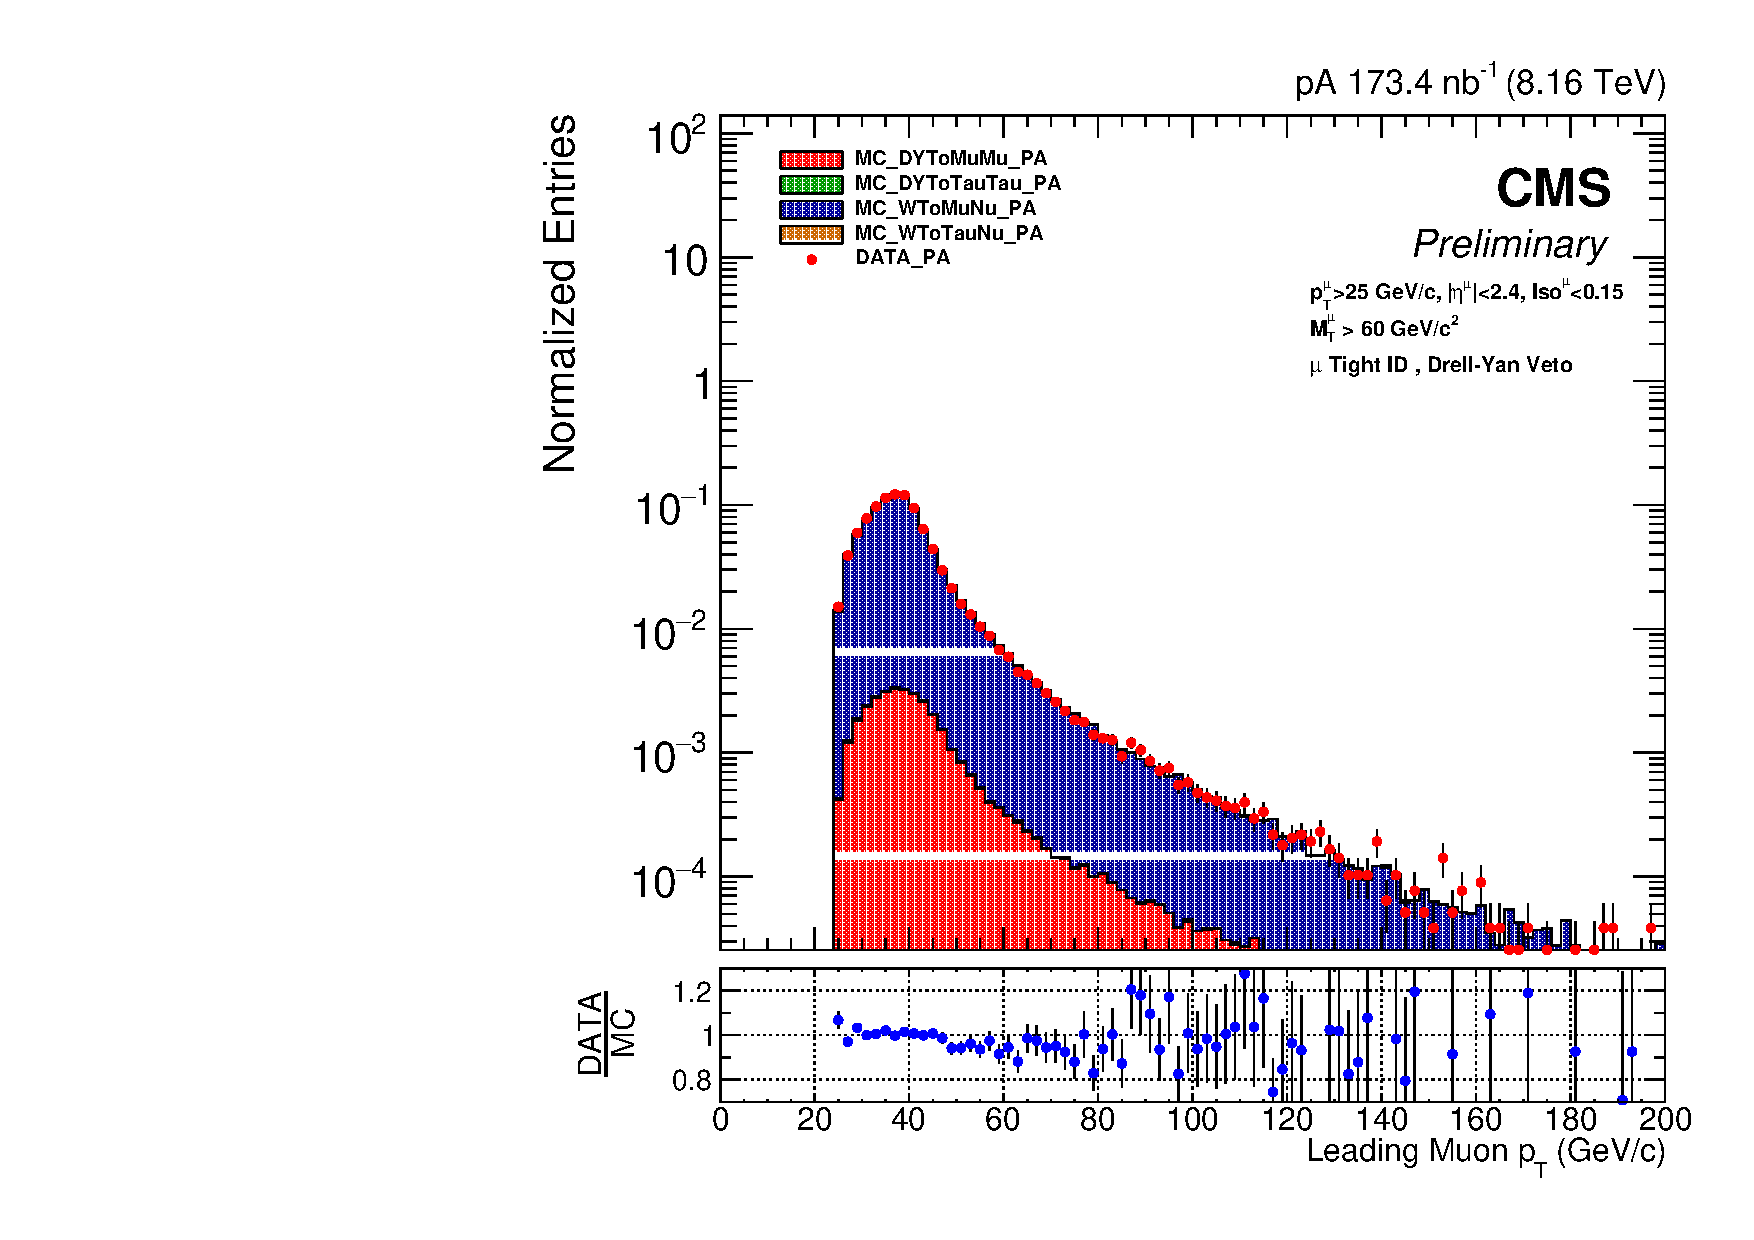
\includegraphics[width=0.45\textwidth]{Figures/WBoson/Analysis/Correction/BosonPT/c_DATAvsMCStack_MC_PA_WToMu_Plus_Mu_PT.pdf}
  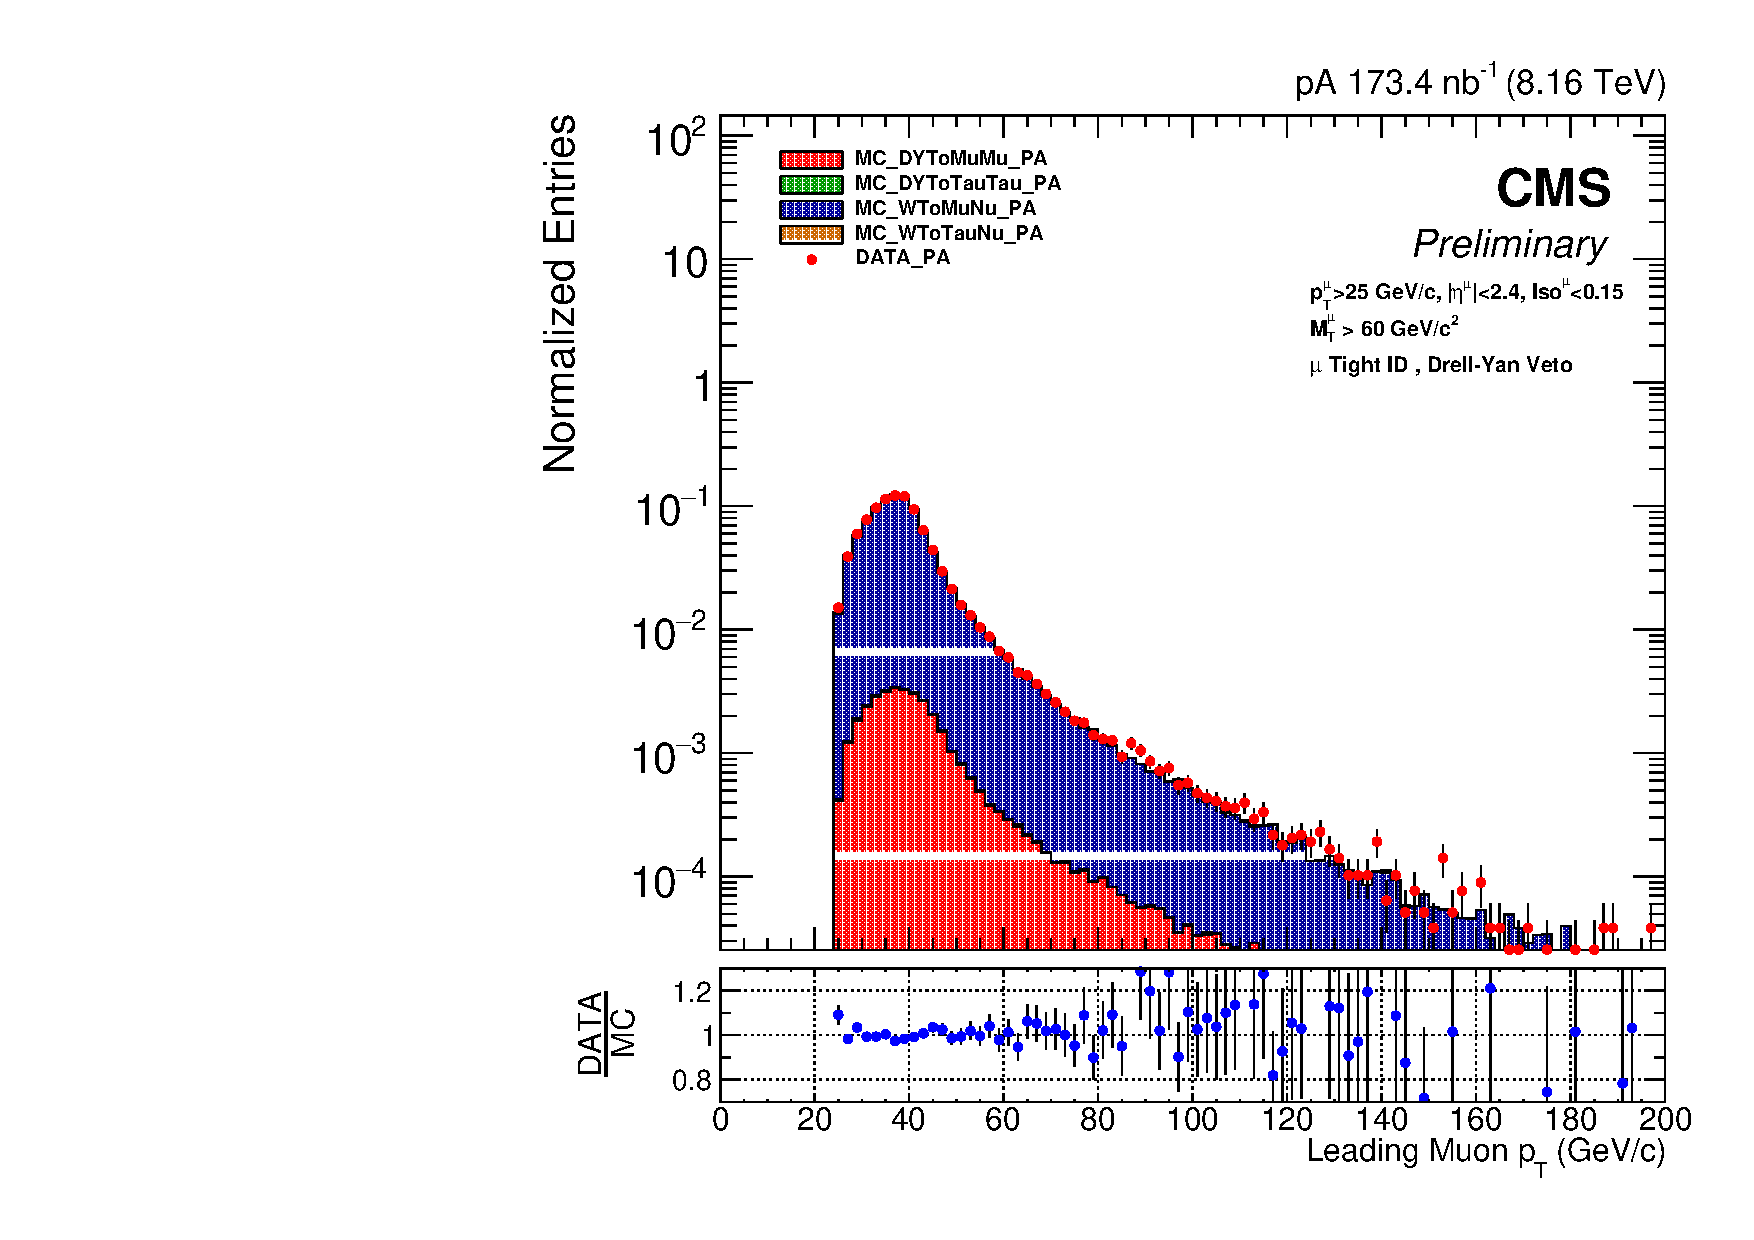
\includegraphics[width=0.45\textwidth]{Figures/WBoson/Analysis/Correction/BosonPT/c_DATAvsMCStack_MC_PA_WToMu_Plus_Mu_PT_NOMINAL.pdf}
 \caption{Muon \pt distribution extracted from the \Wb-boson enhanced sample before (left) and after (right) applying the boson \pt weights. The red points correspond to data, while the blue and red filled areas correspond to events from the \WToMuNu and \DYToMuMu simulations, respectively. The bottom panels shows the ratio of data over simulation.}
 \label{fig:WEventPTDist}
\end{figure}


\subsection{Corrections for missing transverse momentum} \label{sec:WBoson_Analysis_Corrections_MET}

Since the \Wb-boson analysis relays on \ptmiss distributions from simulations to extract the signal, it is important that the simulated \ptmiss describes the data. To achieve this, the \pt distribution of the reconstructed particles, including those recoiling against the weak boson (referred as the recoil), have to be well modelled.

The \ptmiss vector derived from \WToMuNu events can be decomposed, according to \eq{eq:MET}, in two parts: the \pt vector of the muon candidate (\ptMuvec) and the \pt vector of the recoil (\utvec), as defined in:

\begin{equation}
 \ptvecmiss = -\left( \utvec + \ptMuvec \right )
 \label{eq:METSep}
\end{equation}

The recoil \utvec is measured via the \ptvec vectorial sum of all particles identified in an event with the PF algorithm \textit{excluding} the muon from the \Wb-boson decay, as given by:

\begin{equation}
 \utvec = \left(\sum_{\text{particles}} \ptvec\right) - \ptMuvec
 \label{eq:recoil}
\end{equation}

The recoil is a complex quantity that includes particles from the hard scattering that balances the \Wb-boson \pt and from the underlying event (e.g. spectator parton interactions and multiple parton scatterings), as well as effects related to the detector (e.g. electronic noise, \pt resolution, reconstruction efficiency and acceptance) and the accelerator (e.g. beam-beam remnants). As a result, the recoil is difficult to simulate precisely in \RunpPb collisions and the mismodelling of the recoil \ut can affect the signal extraction.

To improve the modelling of the \ptmiss in the signal region, the \ptmiss is corrected in two steps. First, the distribution of the simulated event activity measured as a function of the total energy deposited in the HF calorimeter (hereafter referred as the HF energy) is weighed to the level observed in data as detailed in \sect{sec:WBoson_Analysis_Corrections_EventActivityReweighing}. Afterwards, the simulated recoil is calibrated following the procedure described in \sect{sec:WBoson_Analysis_Corrections_RecoilCalib}.

\subsubsection{Event activity weighing}\label{sec:WBoson_Analysis_Corrections_EventActivityReweighing}

The muon isolation and the \ptmiss are computed by summing over particles produced in the event. As a consequence, any disagreement in the modelling of the event activity (EA) can impact the muon efficiency and the signal extraction. The disagreement between data and the \POWHEG simulations embedded in \EPOS minimum bias events can be caused by the presence of hard probes such as \Wb bosons, which bias the event activity towards higher particle  multiplicity compared to minimum bias events.

To check if the event activity is well modelled in the simulations, the distribution of the number of tracks per event and the HF energy is compared between data and simulation in a \ZToMuMu control sample. The \ZToMuMu events are selected by requiring a \mumu pair within the invariant mass region $80 < M_{\mumu} < 110$~\GeVcc as detailed in \sect{sec:WBoson_Analysis_Selection_WSelection}. The data-simulation comparisons are shown in \fig{fig:HFNoCorr}, and it is observed that the simulated samples are indeed not able to reproduce the event activity present in \RunpPb data.

\begin{figure}[htb!]
 \centering
  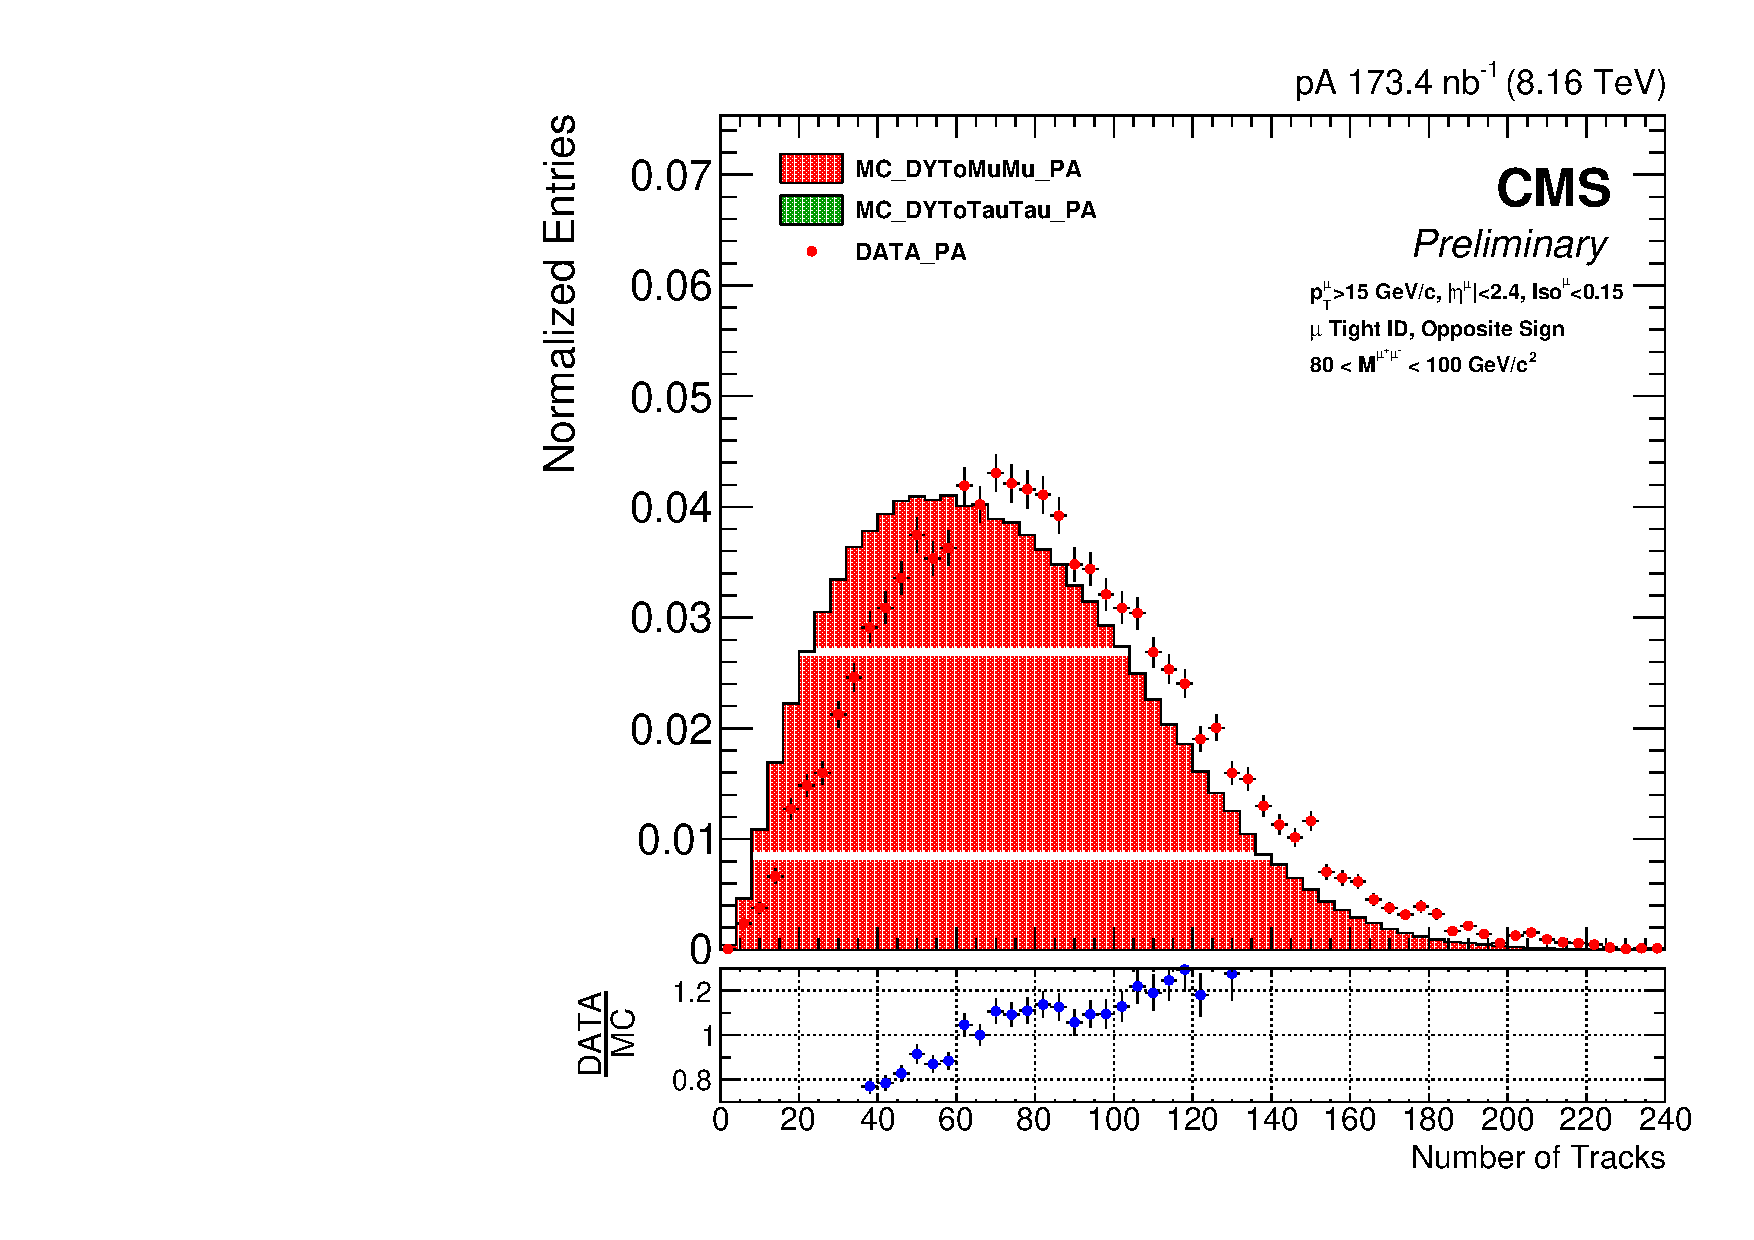
\includegraphics[width=0.40\textwidth]{Figures/WBoson/Analysis/Correction/EventActivityReweighing/c_DATAvsMCStack_MC_PA_ZToMuMu_Track_N.pdf}
  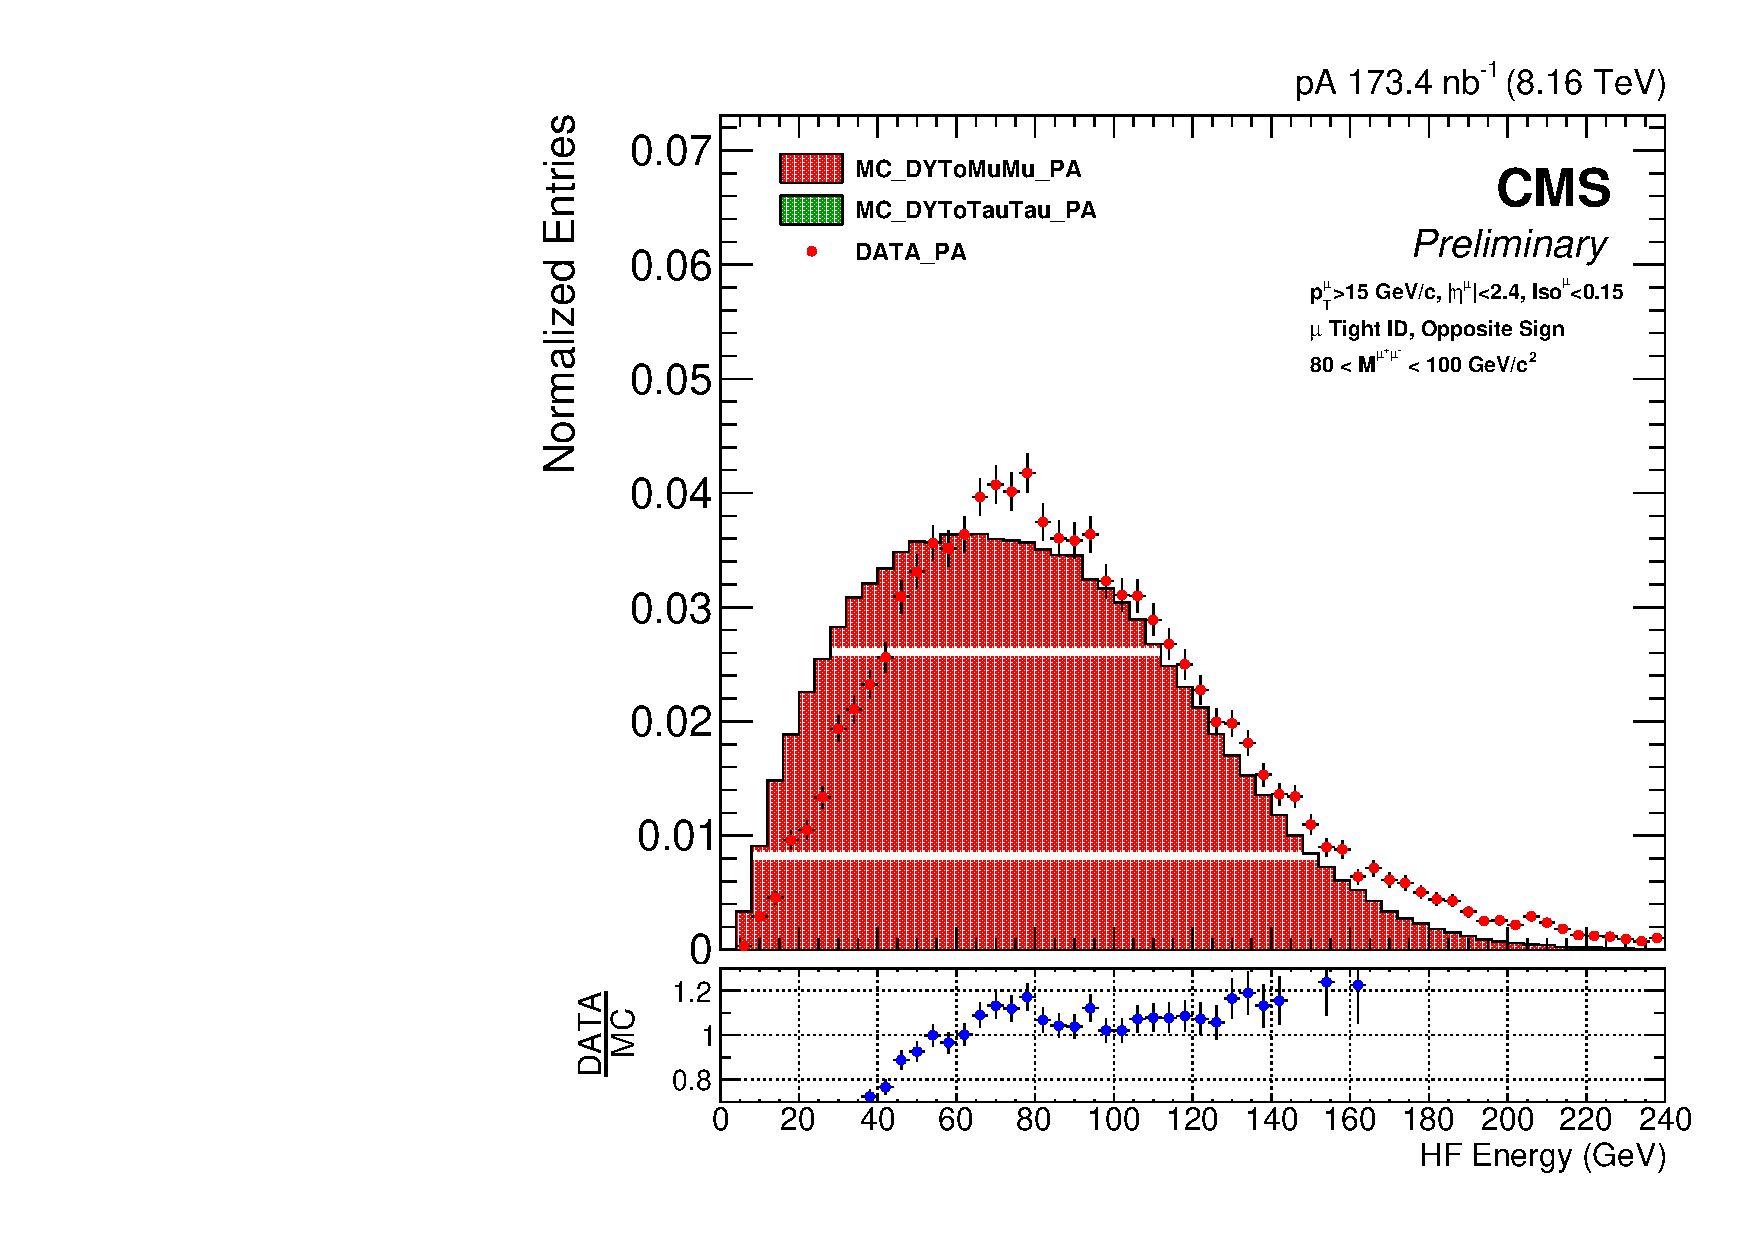
\includegraphics[width=0.40\textwidth]{Figures/WBoson/Analysis/Correction/EventActivityReweighing/c_DATAvsMCStack_MC_PA_ZToMuMu_HF_E.pdf}
 \caption{Distribution of the number of tracks per event (left) and the total energy deposited in the HF calorimeter (right) in \ZToMuMu events. The red points and filled area correspond to data and \DYToMuMu simulation, respectively.}
 \label{fig:HFNoCorr}
\end{figure}

The modelling of the event activity is improved using a set of weights determined from the ratio of the number of \ZToMuMu events extracted from data and simulation in different bins of HF energy ($E_{\text{HF}}$), as given by:

\begin{equation}
 w^{\text{EA}}\left(E_{\text{HF}}\right) = \frac{N_{\ZToMuMu}^{\text{data}}\left[E_{\text{HF}}\right]}{N_{\ZToMuMu}^{\text{MC}}\left[E_{\text{HF}}\right]}
\end{equation}

The $w^{\text{EA}}\left(E_{\text{HF}}\right)$ weights are used, event-by-event, to weigh the HF energy distribution of the electroweak and \ttbar simulations. \fig{fig:HFrewCheck} shows that the HF energy weighing improves the simulation-to-data agreement of the \ptmiss distribution of \ZToMuMu events. The remaining level of disagreement in the \ptmiss is then corrected for by calibrating the simulated recoil as explained in the next section.

\begin{figure}[htb!]
 \centering
 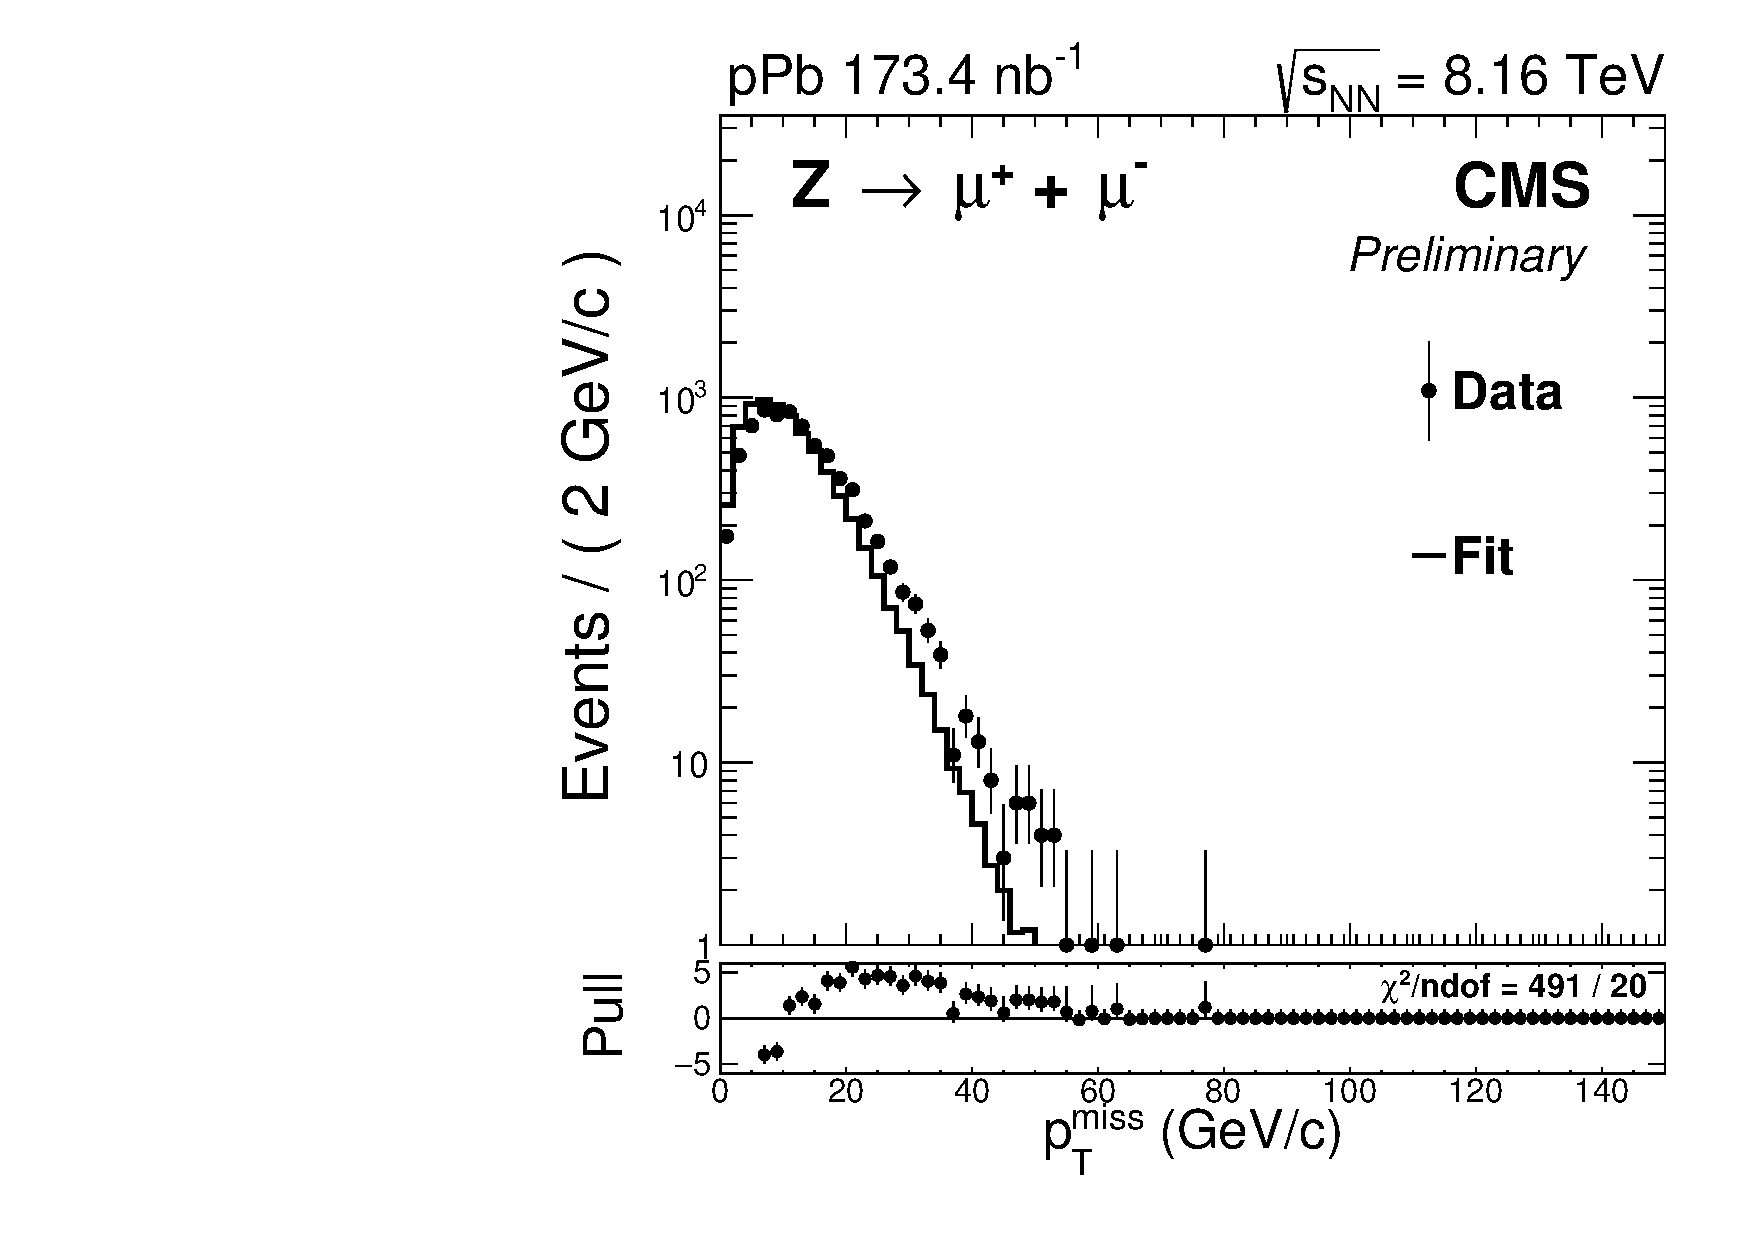
\includegraphics[width=0.4\textwidth]{Figures/WBoson/Analysis/Correction/Recoil/CheckFits/Z/METPF_RAW/PLOT_MET_DATA_ZToMuPl_PA_Model_TEMP_DY_MuEtaCM_-286_193_MuIso_0_15.pdf}
 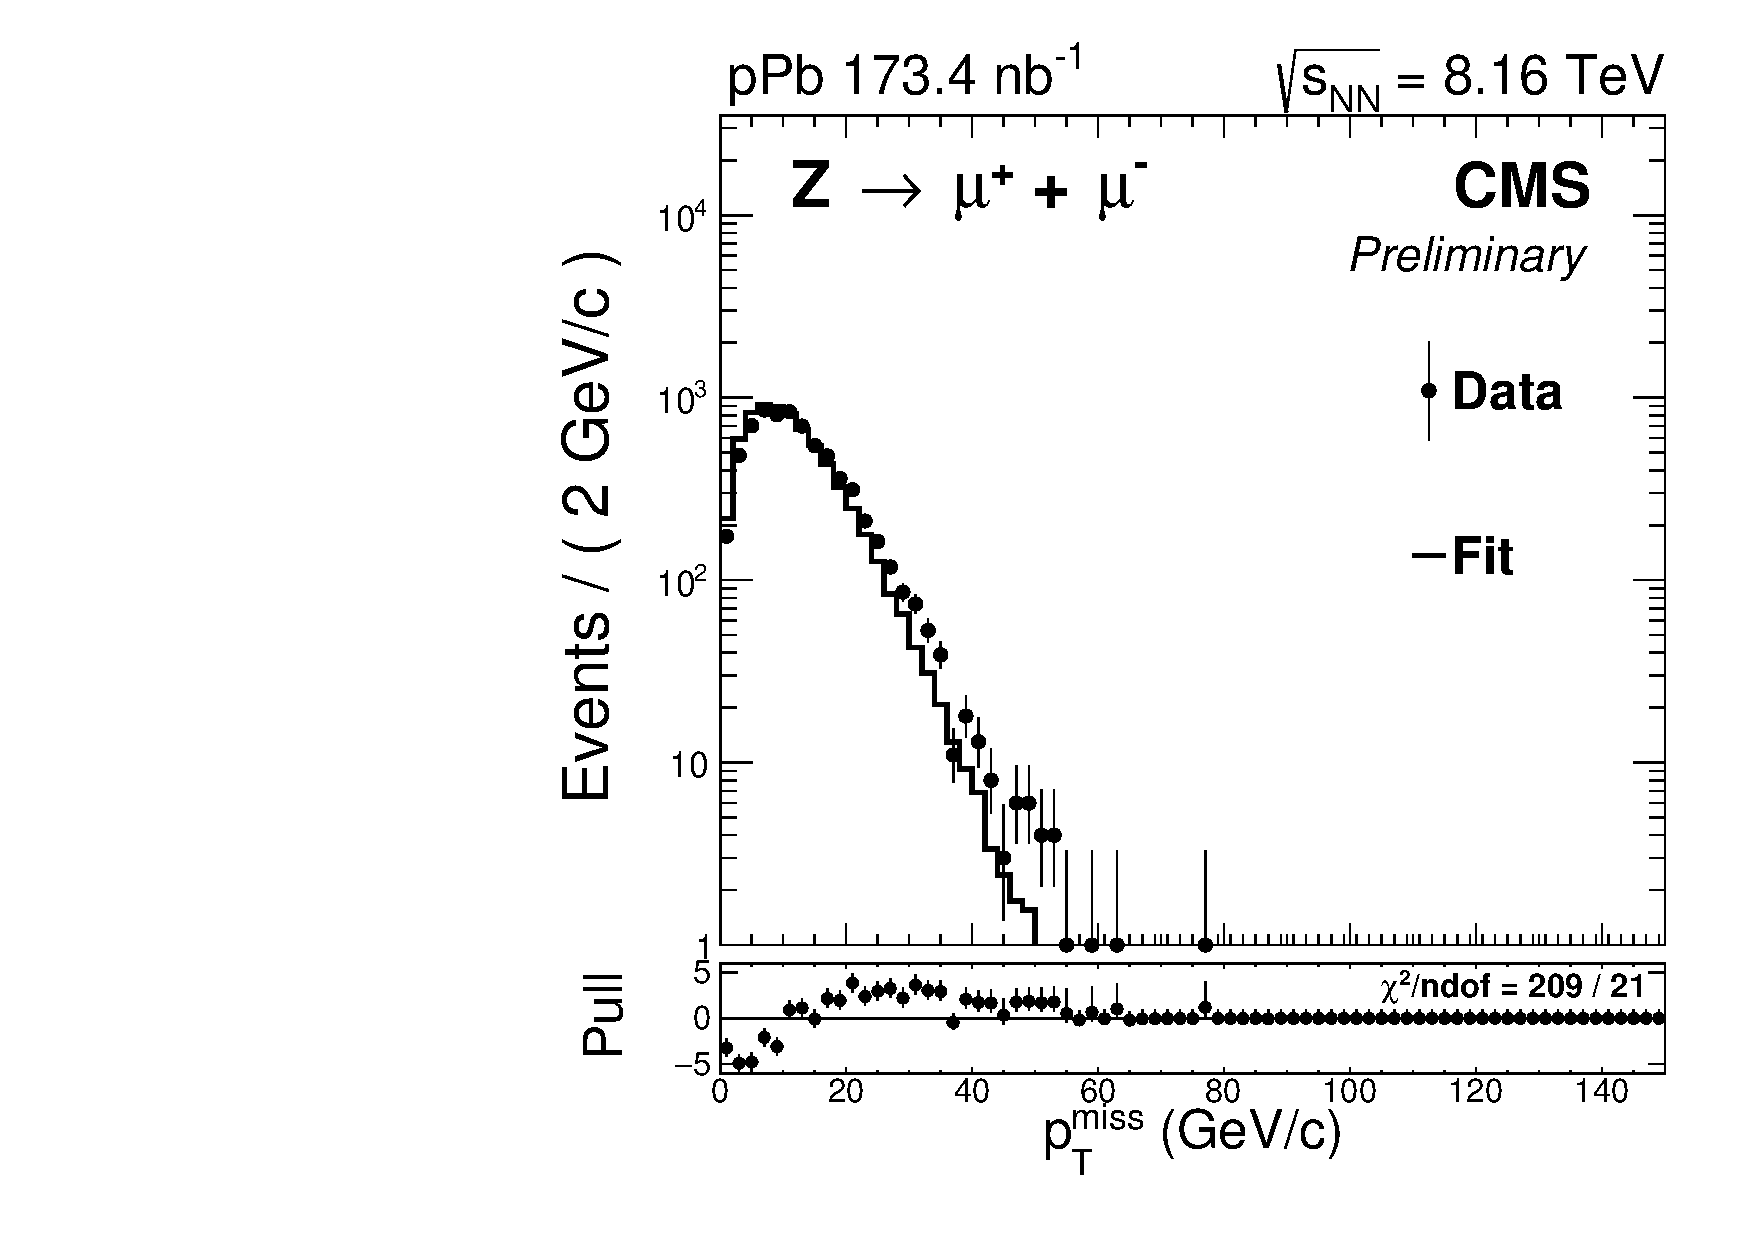
\includegraphics[width=0.4\textwidth]{Figures/WBoson/Analysis/Correction/Recoil/CheckFits/Z/METPF_RAW_HFrew/PLOT_MET_DATA_ZToMuPl_PA_Model_TEMP_DY_MuEtaCM_-286_193_MuIso_0_15.pdf}
 \caption{Comparison of the \ptmiss distribution in data and simulation for \ZToMuMu events before (left) and after (right) applying the HF energy weights.}
 \label{fig:HFrewCheck}
\end{figure}


\subsubsection{Recoil calibration} \label{sec:WBoson_Analysis_Corrections_RecoilCalib}

The recoil calibration procedure starts by measuring the recoil in \ZToMuMu events in data and simulation, and then parametrise, in each sample, the components of the recoil \utvec with respect to the transverse momentum of the \Z boson (\qtZ). Afterwards, these parametrisations are used to scale in each event the simulated \utvec components according to the weak boson \pt, from each electroweak simulation, to match the average recoil distribution measured in data.

The \ZToMuMu control sample employed to extract the recoil calibration is the same as the one used to derive  the event activity weights described in the previous section. In addition, the simulated HF energy and the generated \Z-boson \pt distributions of the control sample have been weighed accordingly.

\paragraph{Extraction of the recoil scale and resolution.} Since there are no neutrinos produced in the initial hard scattering of \ZToMuMu events, the \ptmiss spectrum can be used to directly measure the \ptmiss resolution. \fig{fig:METZBoson} compares the \ptmiss spectra extracted from data and simulation in the \ZToMuMu control sample. It is observed that the simulation does not properly describe the \ptmiss distribution measured in data.

\begin{figure}[htb!]
 \centering
 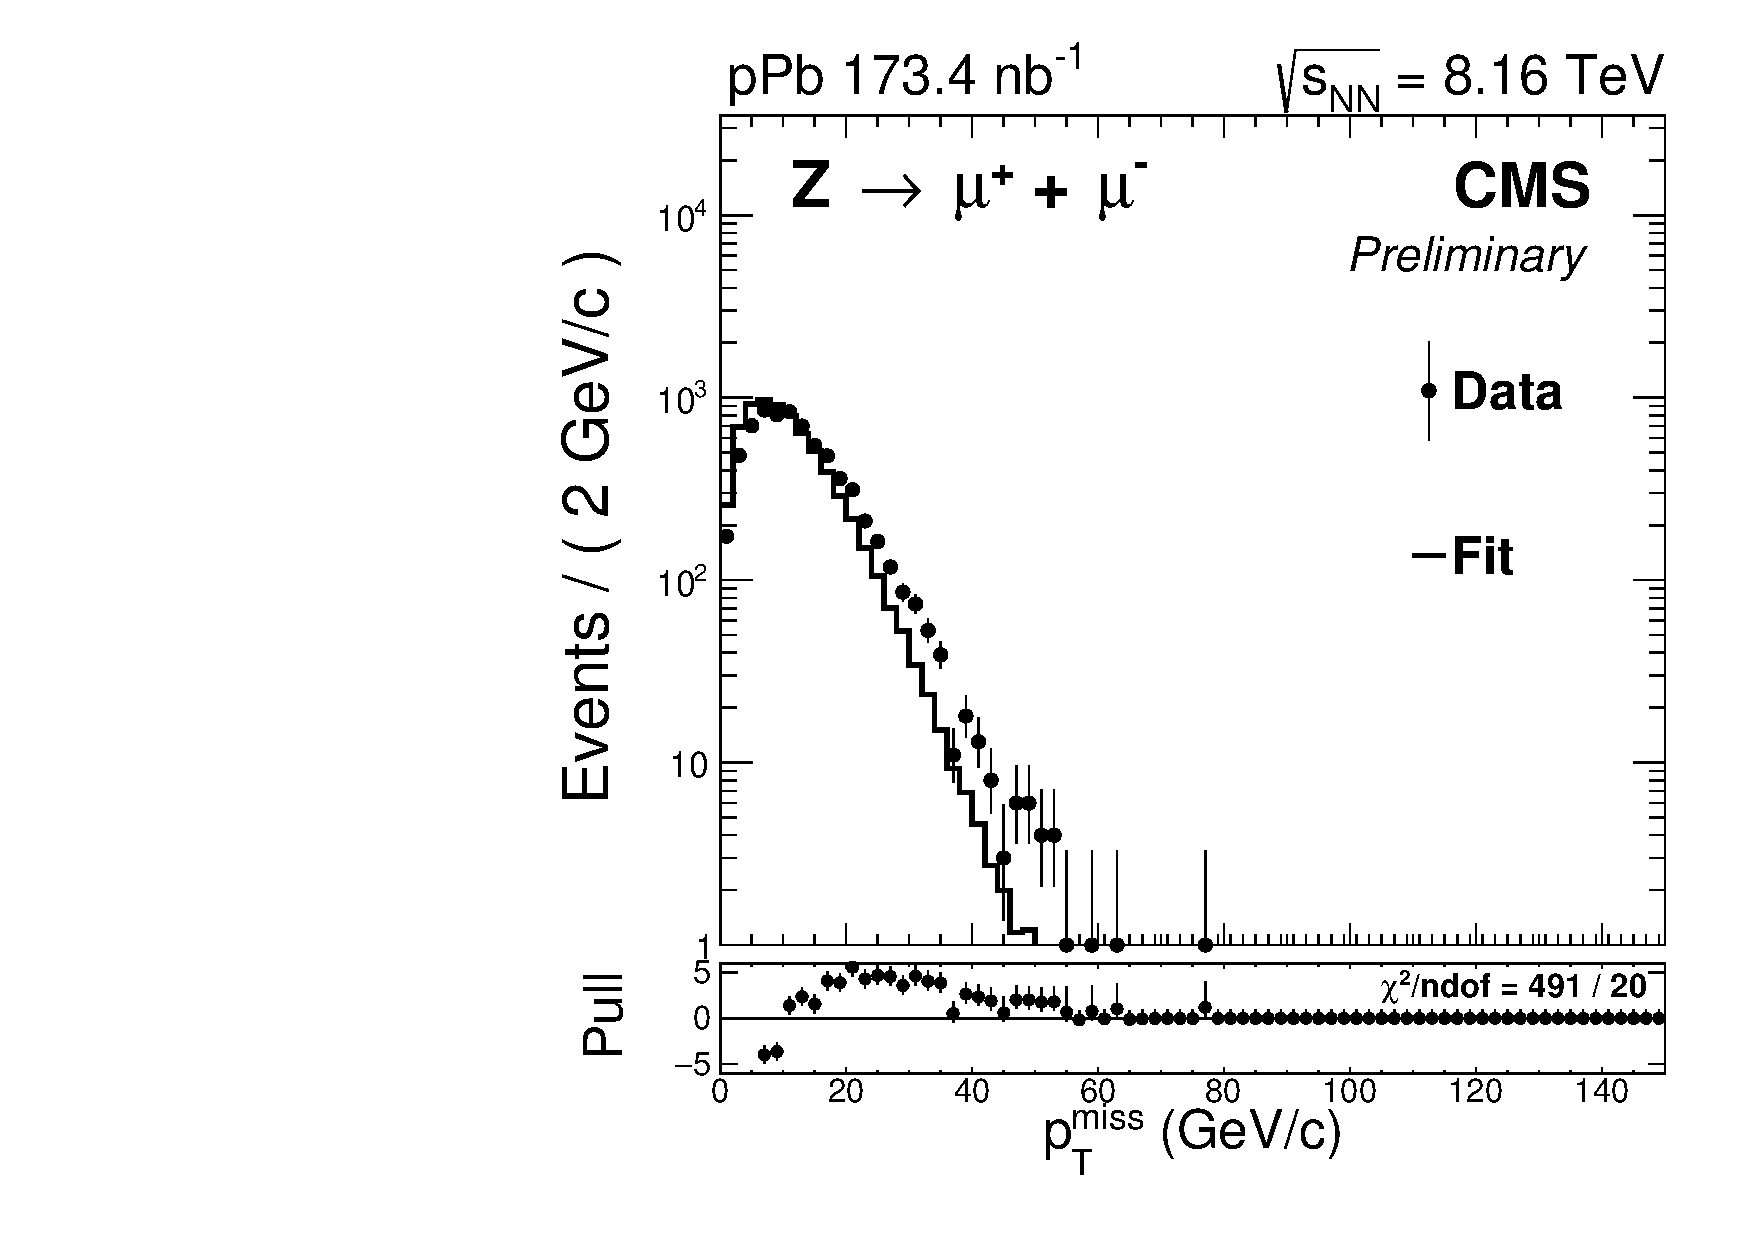
\includegraphics[width=0.5\textwidth]{Figures/WBoson/Analysis/Correction/Recoil/CheckFits/Z/METPF_RAW/PLOT_MET_DATA_ZToMuPl_PA_Model_TEMP_DY_MuEtaCM_-286_193_MuIso_0_15.pdf}
 \caption{Distribution of the \ptmiss in data and simulation for \ZToMuMu selected events.}
 \label{fig:METZBoson}
\end{figure}

In the case of \ZToMuMu events, the recoil \utvec is measured by \textit{subtracting} the \pt vector of the \Z-boson candidate ($\qtZvec = \ptvec^{\mu^{+}} + \ptvec^{\mu^{-}}$) from the \ptvecmiss, according to:

\begin{equation}
 \utvec = -\ptvecmiss - \qtZvec
 \label{eq:recoilZBoson}
\end{equation}

The recoil \utvec is then projected along the \Z-boson \qtZvec direction. The parallel and perpendicular components of \utvec, with respect to the \qtZvec, are labelled as \utpar and \utper, respectively. \fig{fig:RecoilComp} shows the components of the recoil in \ZToMuMu events.

\begin{figure}[htb!]
 \centering
 \begin{tikzpicture}
  \draw[dashed, thick] (-4.4,0)--(4.4,0) node[right]{};
  \draw[dashed, thick] (0,-3.0)--(0,3.0) node[above]{};
  \draw[line width=2pt,black,-stealth](0,0)--(-2.8,-1.2) node[anchor=north west]{\utvec};
  \draw[line width=1pt,black,-stealth](-2.8,0)--(-2.8,-1.2) node[anchor=south east]{\utpar};
  \draw[line width=1pt,black,-stealth](0,0)--(-2.8,0) node[anchor=south west]{\utper};
  \draw[dashed,->,black,thick](0,0)--(-1.2,1.2) node[anchor=south east]{\ptvecmiss};
  \draw[line width=1pt,black,-stealth](0,0)--(2,-2) node[anchor=south west]{$\ptvec\left(\mu^{+}\right)$};
  \draw[line width=1pt,black,-stealth](0,0)--(2,2) node[anchor=south west]{$\ptvec\left(\mu^{-}\right)$};
  \draw[line width=3pt,black,-stealth](0,0)--(4,0) node[anchor=south west]{$\qtvec\left(\text{Z}\right)	$};
 \end{tikzpicture}
 \caption{Definition and components of the recoil \utvec for \ZToMuMu events.}
 \label{fig:RecoilComp}
\end{figure}

The \utpar and \utper recoil components are evaluated event-by-event and sorted in 30 bins of \qtZ defined within the range $0 < \qtZ < 140$~\GeVc. The distributions of \utpar and \utper from data and simulation are fitted separately in each \qtZ bin with a weighed sum of two Gaussian functions, according to:

\begin{equation}
 \begin{aligned}
  F\left(u_{\parallel}\right) &= N_{\parallel} \cdot \left( f_{\parallel} \cdot  \exp\left[{\frac{\left(u_{\parallel} - \mu_{\parallel}\right)^{2}}{2 \cdot \sigma_{\parallel,1}^{2}}}\right]  + \left(1-f_{\parallel}\right)\cdot \exp\left[{\frac{\left(u_{\parallel} - \mu_{\parallel}\right)^{2}}{2 \cdot \sigma_{\parallel,2}^{2}}}\right]  \right) \\
  F\left(u_{\perp}\right) &= N_{\perp} \cdot \left( f_{\perp} \cdot  \exp\left[{\frac{\left(u_{\perp} - \mu_{\perp}\right)^{2}}{2 \cdot \sigma_{\perp,1}^{2}}}\right]  + \left(1-f_{\perp}\right)\cdot \exp\left[{\frac{\left(u_{\perp} - \mu_{\perp}\right)^{2}}{2 \cdot \sigma_{\perp,2}^{2}}}\right]  \right)
 \end{aligned}
 \label{eq:gaussFit}
\end{equation}

where $N_{\parallel(\perp)}$ corresponds to the number of events in each \qtZ bin, $f_{\parallel(\perp)}$ is the weight of the Gaussian components, $\mu_{\parallel(\perp)}$ is the mean of the Gaussian functions, and $\sigma_{\parallel(\perp),1}$ and $\sigma_{\parallel(\perp),2}$ are the corresponding Gaussian widths. The parameters $f_{\parallel}$ and $f_{\perp}$ are fixed to: $f_{\parallel} = f_{\perp} = 0.70$ in data and $f_{\parallel} = f_{\perp} = 0.45$ in simulation, to obtain a better convergence of the fits. The other parameters are left free.

Examples of the distributions of the parallel and perpendicular recoil components are shown in \fig{fig:RecoilFits} for data and simulation. Also, the fits performed with the weighed combination of Gaussian functions and their pull distributions are presented.

\begin{figure}[htb!]
 \centering
 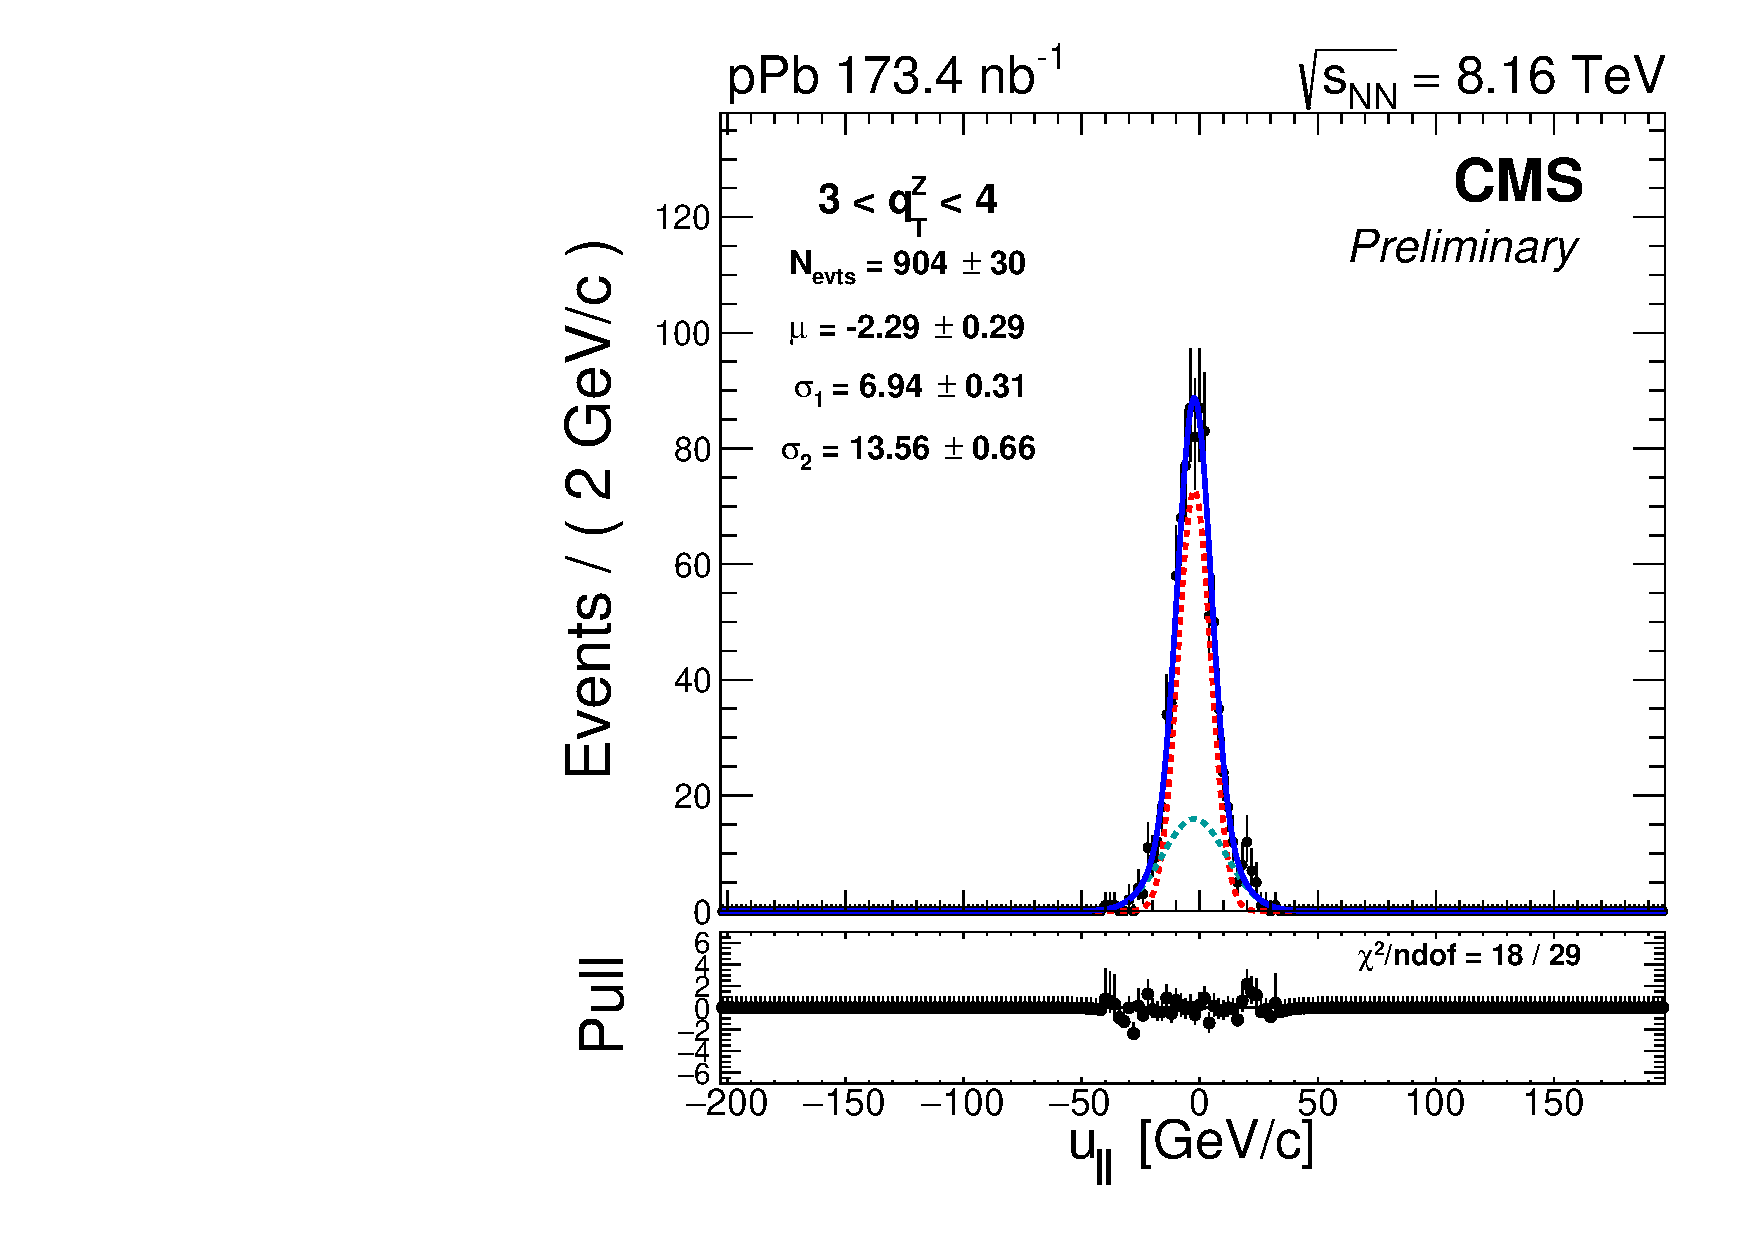
\includegraphics[width=0.4\textwidth]{Figures/WBoson/Analysis/Correction/Recoil/RecoilFits/Data/pfu1fit_2.pdf}
 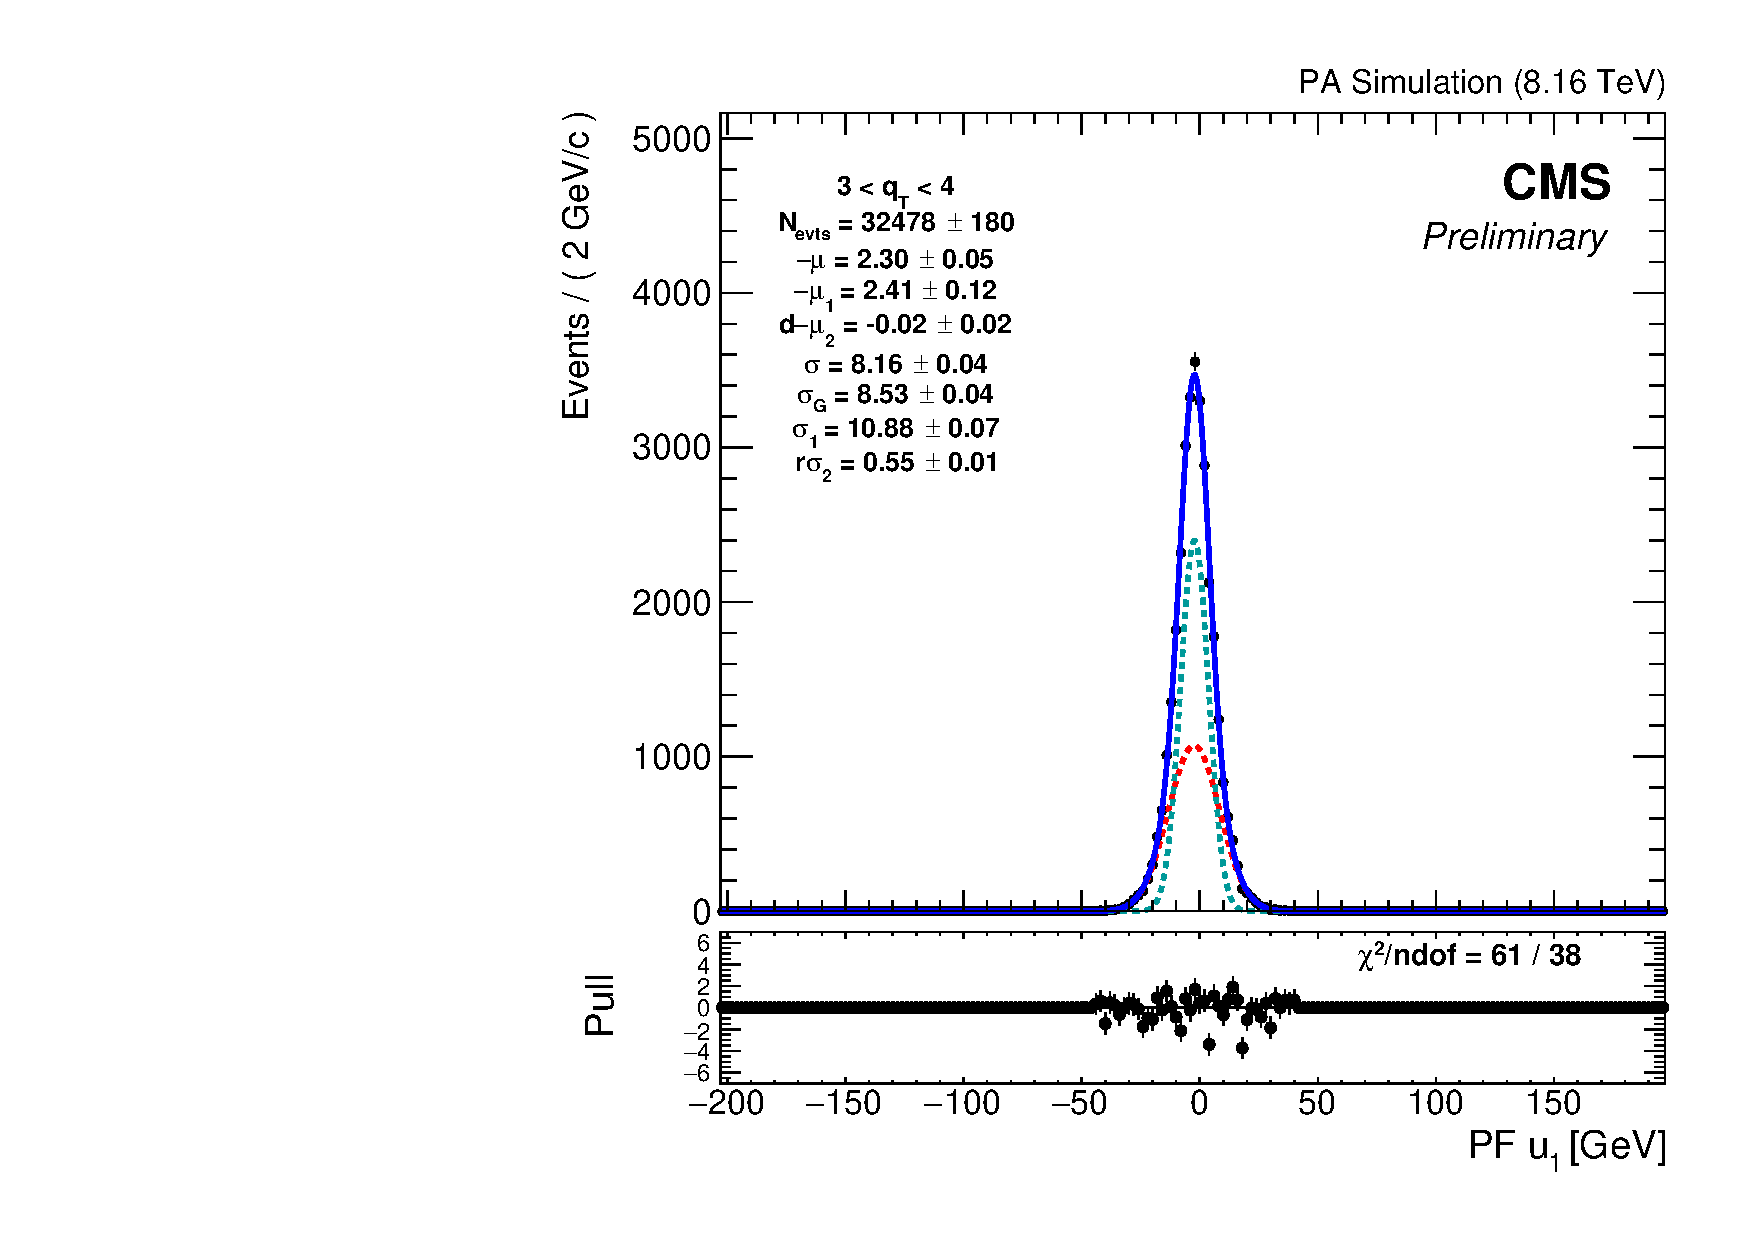
\includegraphics[width=0.4\textwidth]{Figures/WBoson/Analysis/Correction/Recoil/RecoilFits/MC/pfu1fit_2.pdf} \\
 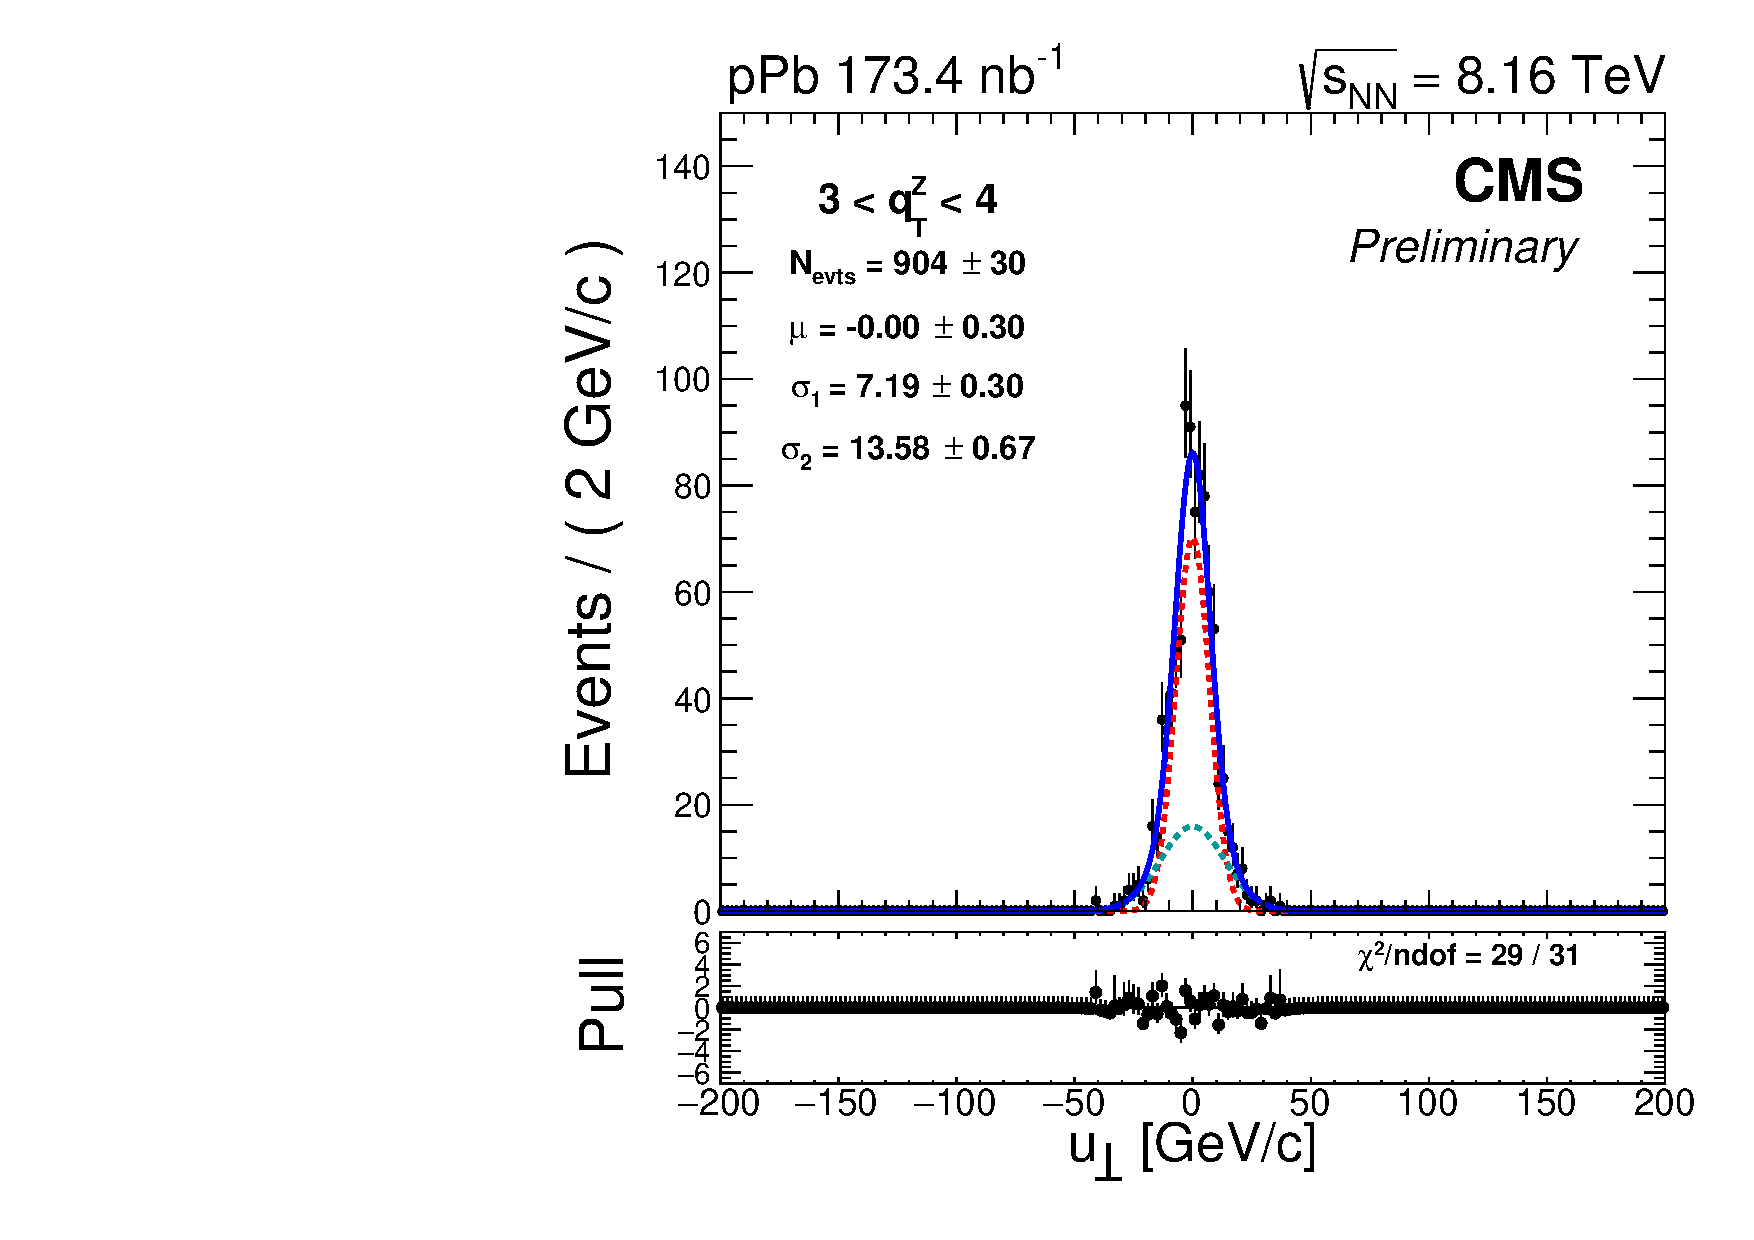
\includegraphics[width=0.4\textwidth]{Figures/WBoson/Analysis/Correction/Recoil/RecoilFits/Data/pfu2fit_2.pdf}
 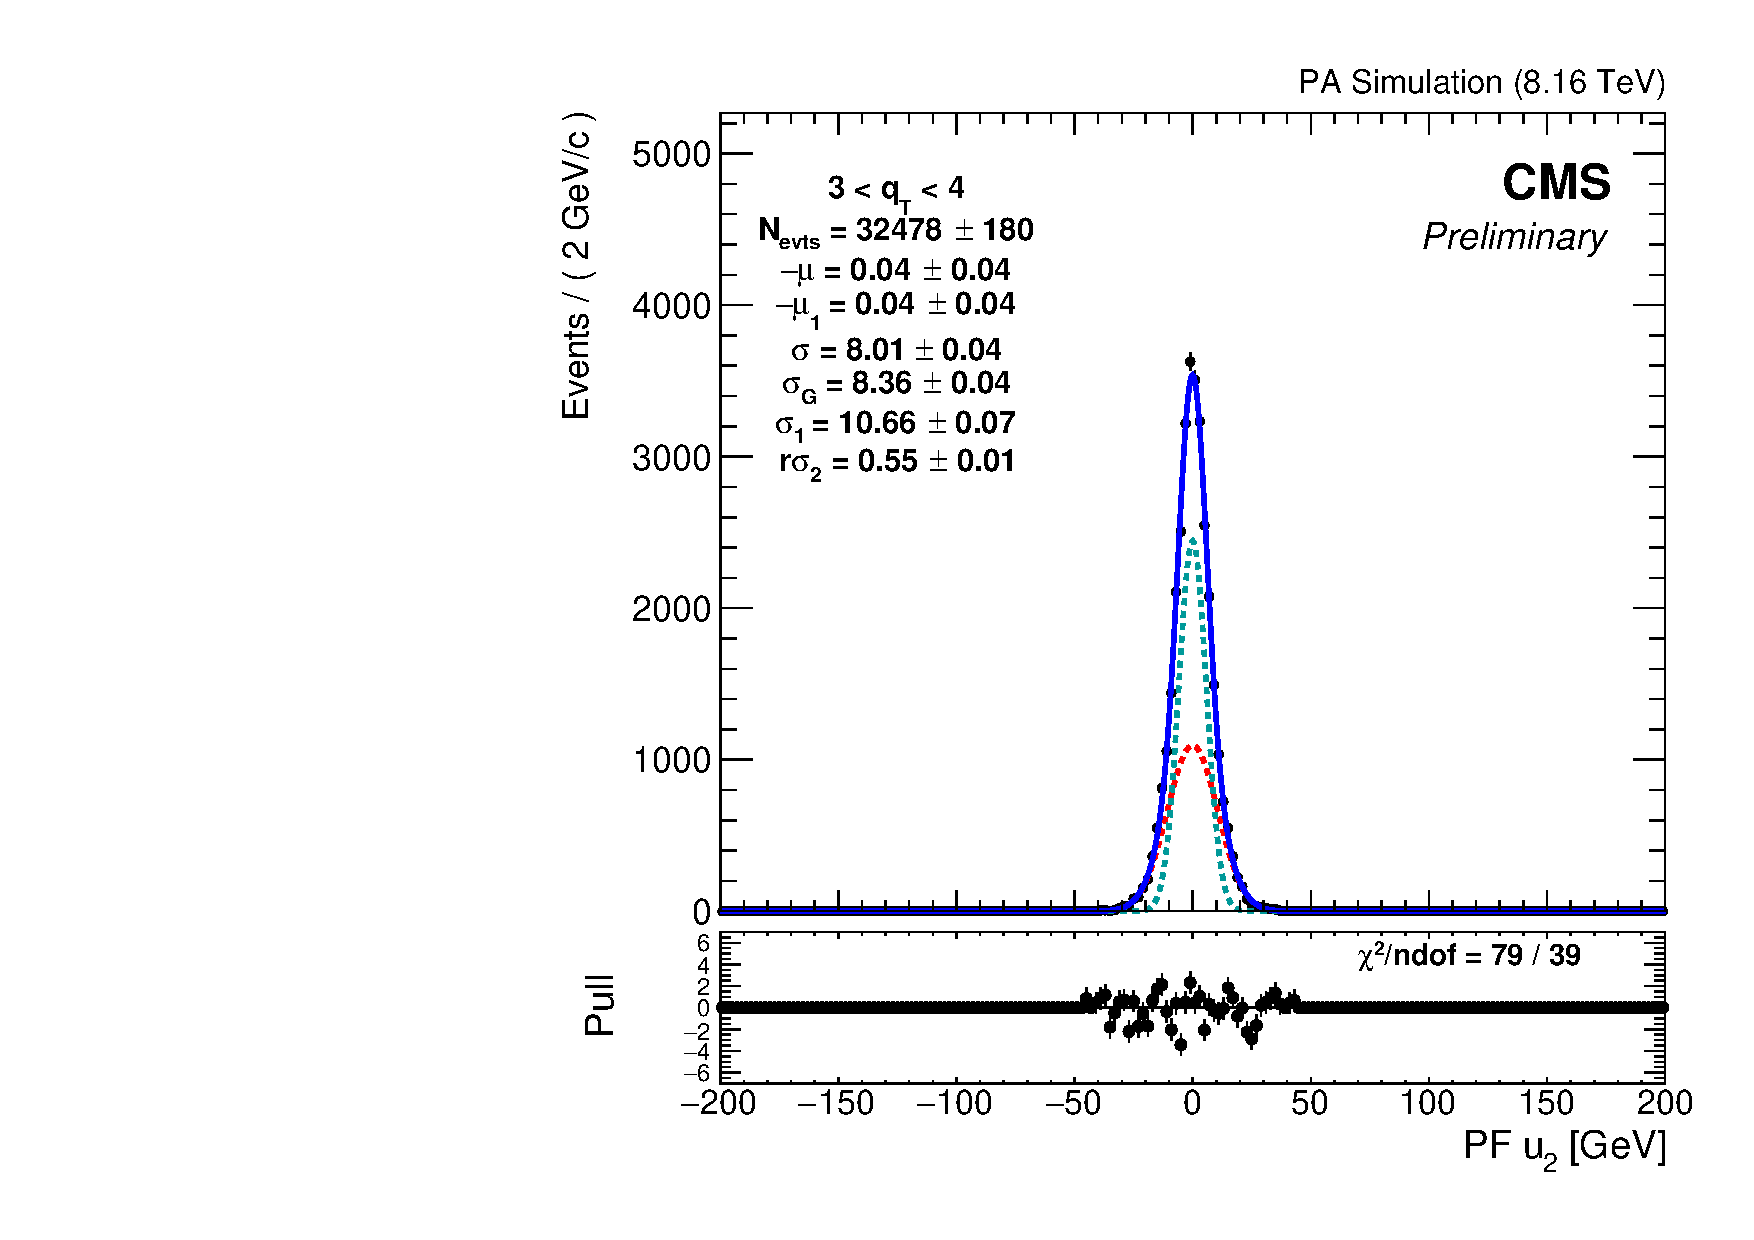
\includegraphics[width=0.4\textwidth]{Figures/WBoson/Analysis/Correction/Recoil/RecoilFits/MC/pfu2fit_2.pdf}
 \caption{Distributions of the \utpar (top) and \utper (bottom) recoil components in data (left) and simulation (right). The fit function is based on a weighted sum of two Gaussian distributions as defined in  in \eq{eq:gaussFit}. The plots correspond to the \qtZ bin [3, 4]~\GeVc.}
 \label{fig:RecoilFits}
\end{figure}

\paragraph{Parameterisation of the recoil scale.} The Gaussian mean parameter $\mu_{\parallel}$ of the recoil parallel component is extracted in each \qtZ bin by fitting the recoil \utper distribution as shown in \fig{fig:RecoilFits}. The profile of $\mu_{\parallel}$ as a function of \qtZ is then fitted using the following function: 

\begin{equation} 
 \mu_{\parallel}\left(\qtZ\right) = -\left(c_{0} + c_{1}\qtZ\right)\left(\frac{1 + \text{Erf}\left[\alpha{\cdot}\left(\qtZ\right)^{\beta}\right]}{2}\right)
 \label{eq:equparparam}
\end{equation}

where $c_{0}$, $c_{1}$, $\alpha$ and $\beta$ are free parameters, and $\text{Erf}(x)$ is the Gaussian error function. These fits are shown in \fig{fig:figU1RecoilScaleFit}, where the sign of $\mu_{\parallel}$ has been reversed to plot the results in the positive y-axis. The slope $c_{1}$ and intercept $c_{0}$ parameters are found to be $c_{1}{\approx}0.9$ and $c_{0}<1.0$~\GeVc, which means that the average \utpar is roughly $10\%$ lower than \qtZ and the contributions at $\qtZ=0$ are negligible. The distributions of the average \utpar for data and simulation are observed to be in good agreement.

\begin{figure}[htb!]
 \centering
 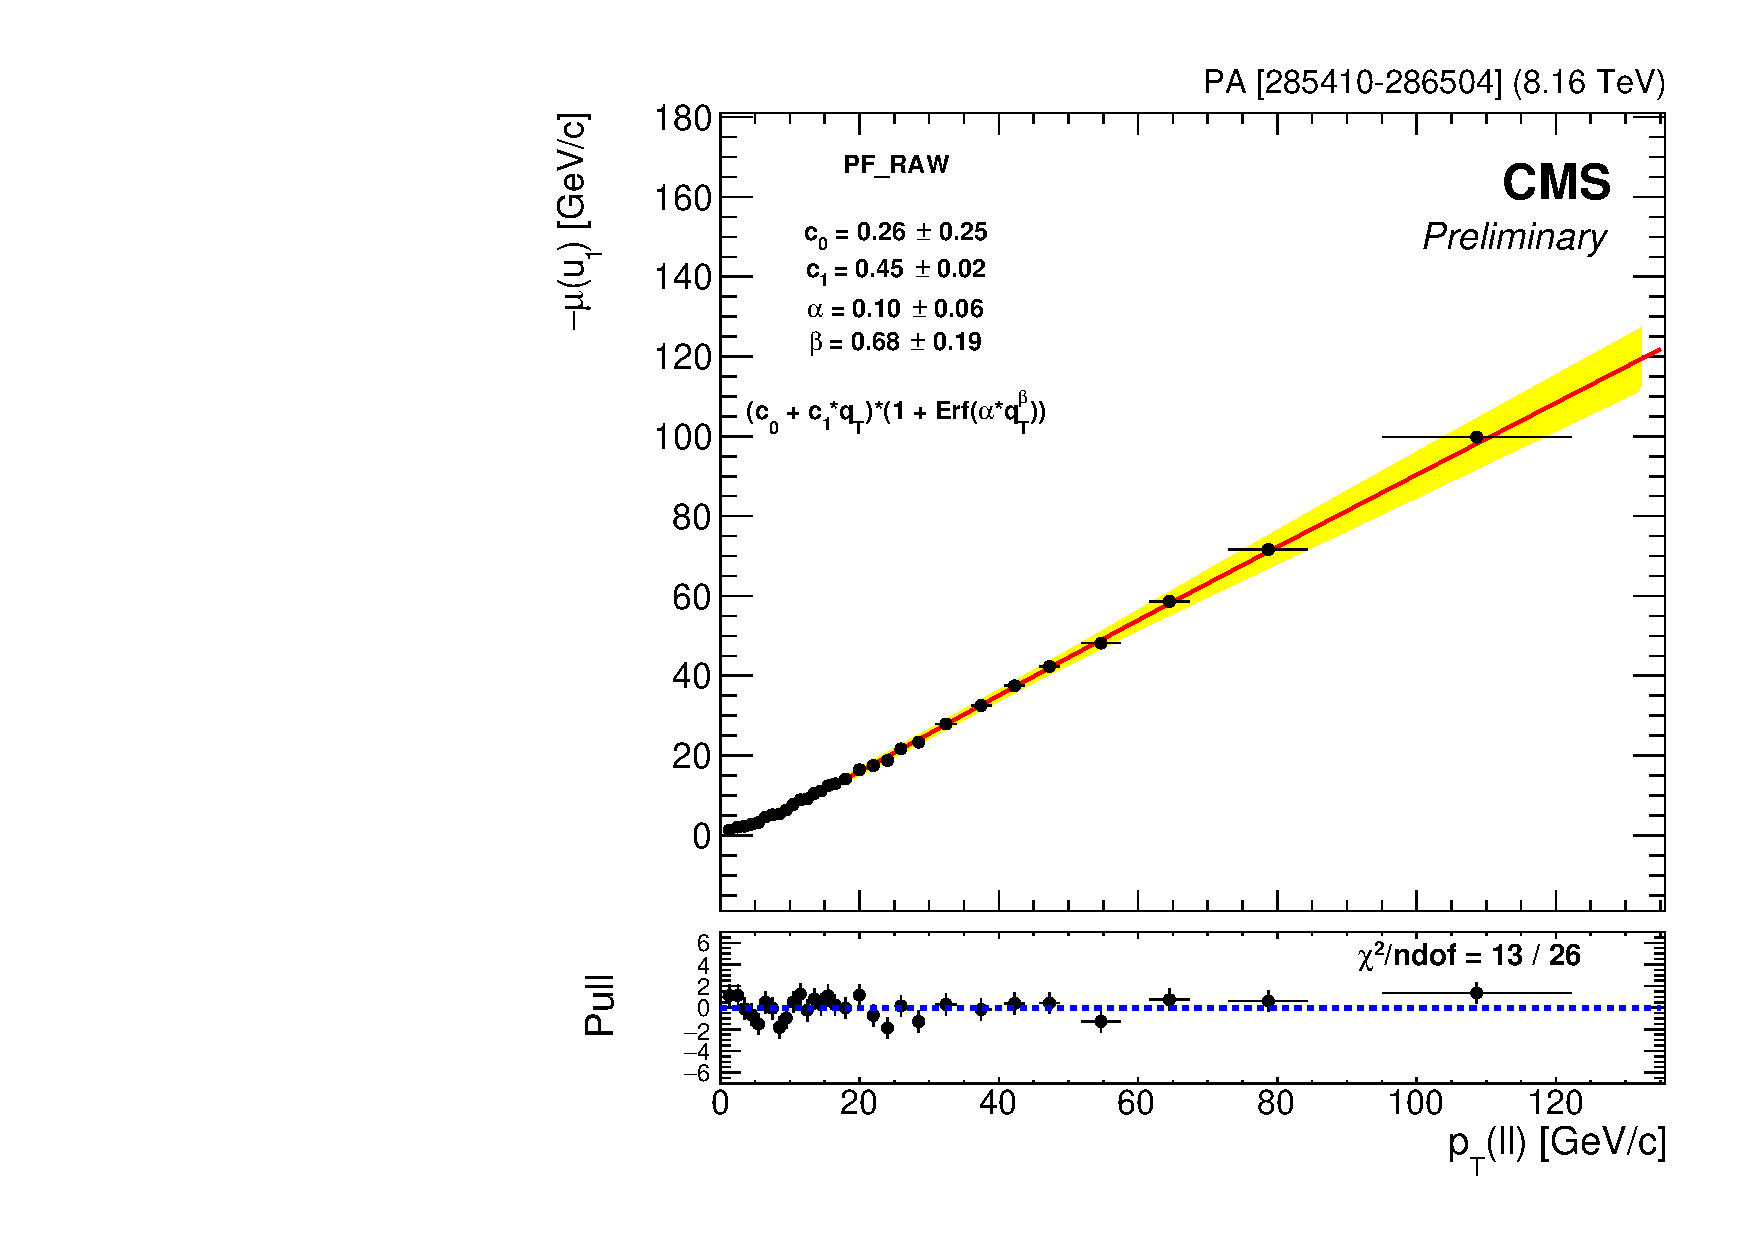
\includegraphics[width=0.45\textwidth]{Figures/WBoson/Analysis/Correction/Recoil/RecoilFitsqT/Data/fitPFu1mean.pdf}
 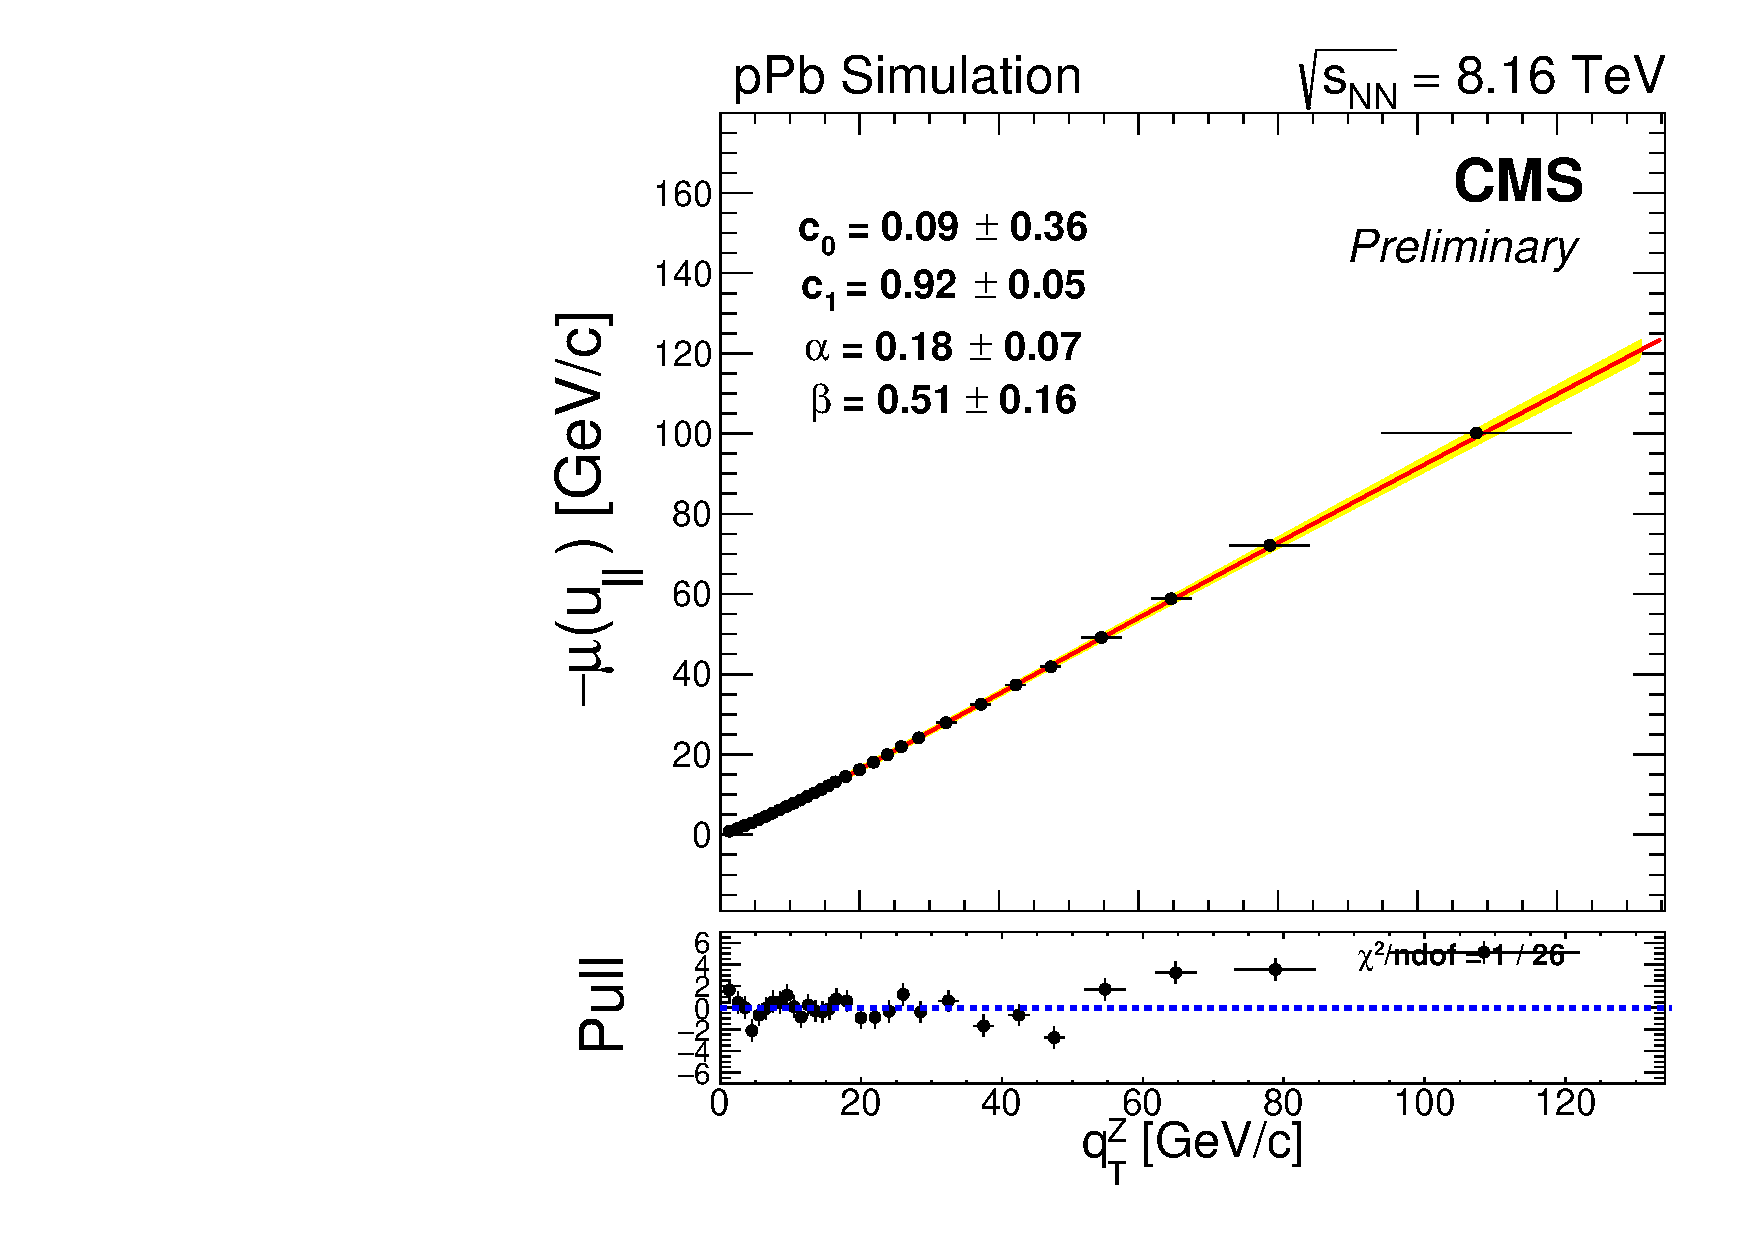
\includegraphics[width=0.45\textwidth]{Figures/WBoson/Analysis/Correction/Recoil/RecoilFitsqT/MC/fitPFu1mean.pdf}
 \caption{Fits of the profile of $-\mu_{\parallel}$ as a function of \qtZ. The results are derived from \ZToMuMu events in data (left) and simulation (right). The yellow band represents the 68\% error band of the  fit.}
 \label{fig:figU1RecoilScaleFit}
\end{figure}

In the case of the perpendicular recoil component, the average \utper value should be zero based on momentum conservation. To check this, the profile of the Gaussian mean parameter $\mu_{\perp}$ as a function of \qtZ is fitted in data and simulation with a constant function:

\begin{equation}
 \mu_{\perp}\left(\qtZ\right) = c_{0}
\end{equation}
 
The outcome of the fits is shown in \fig{fig:figU2RecoilScaleFit}. As expected, the $\mu_{\perp}$ is found to be consistent with zero in simulation and data, showing that there is no bias that affects the average value of the recoil component perpendicular to \qtZvec. From now on, $\mu_{\perp}$ is fixed to zero.

\begin{figure}[htb!]
 \centering
 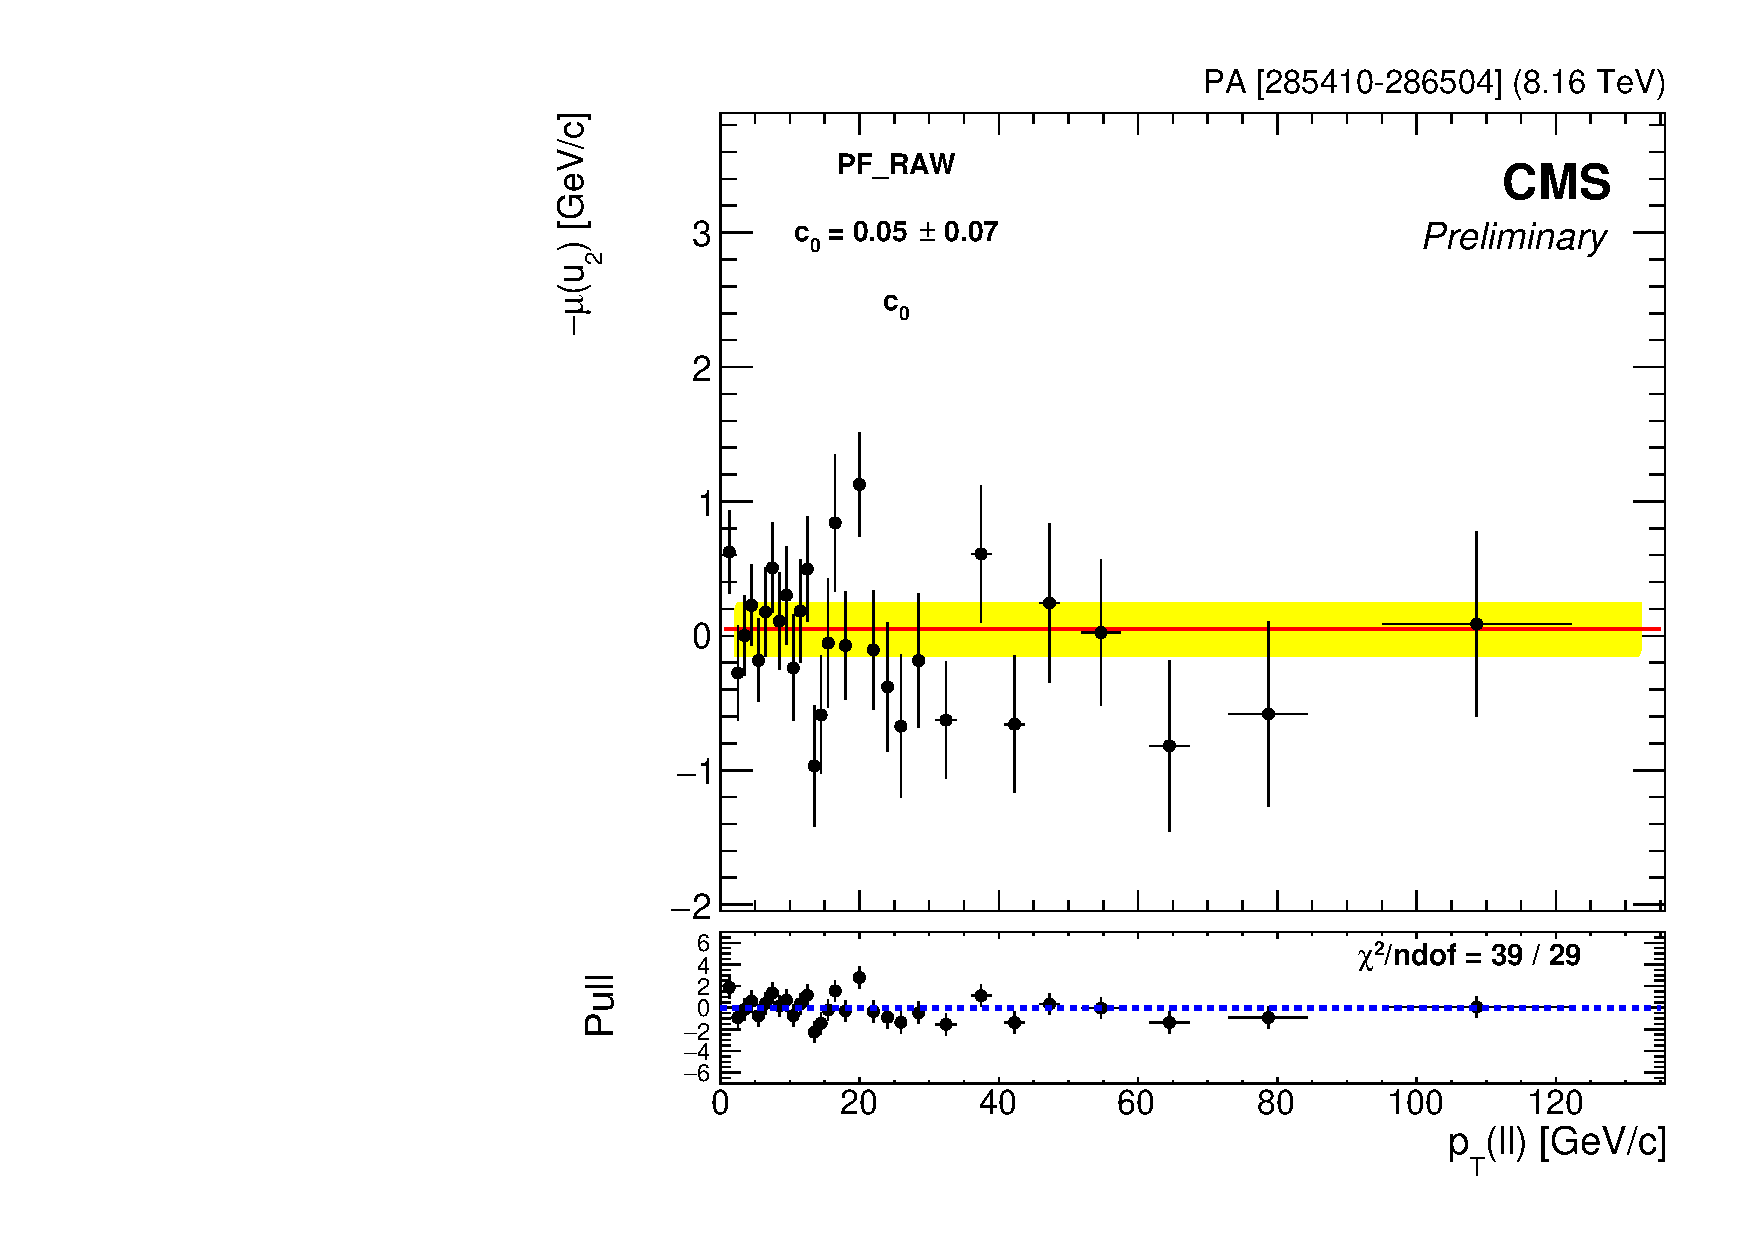
\includegraphics[width=0.45\textwidth]{Figures/WBoson/Analysis/Correction/Recoil/RecoilFitsqT/Data/fitPFu2mean.pdf}
 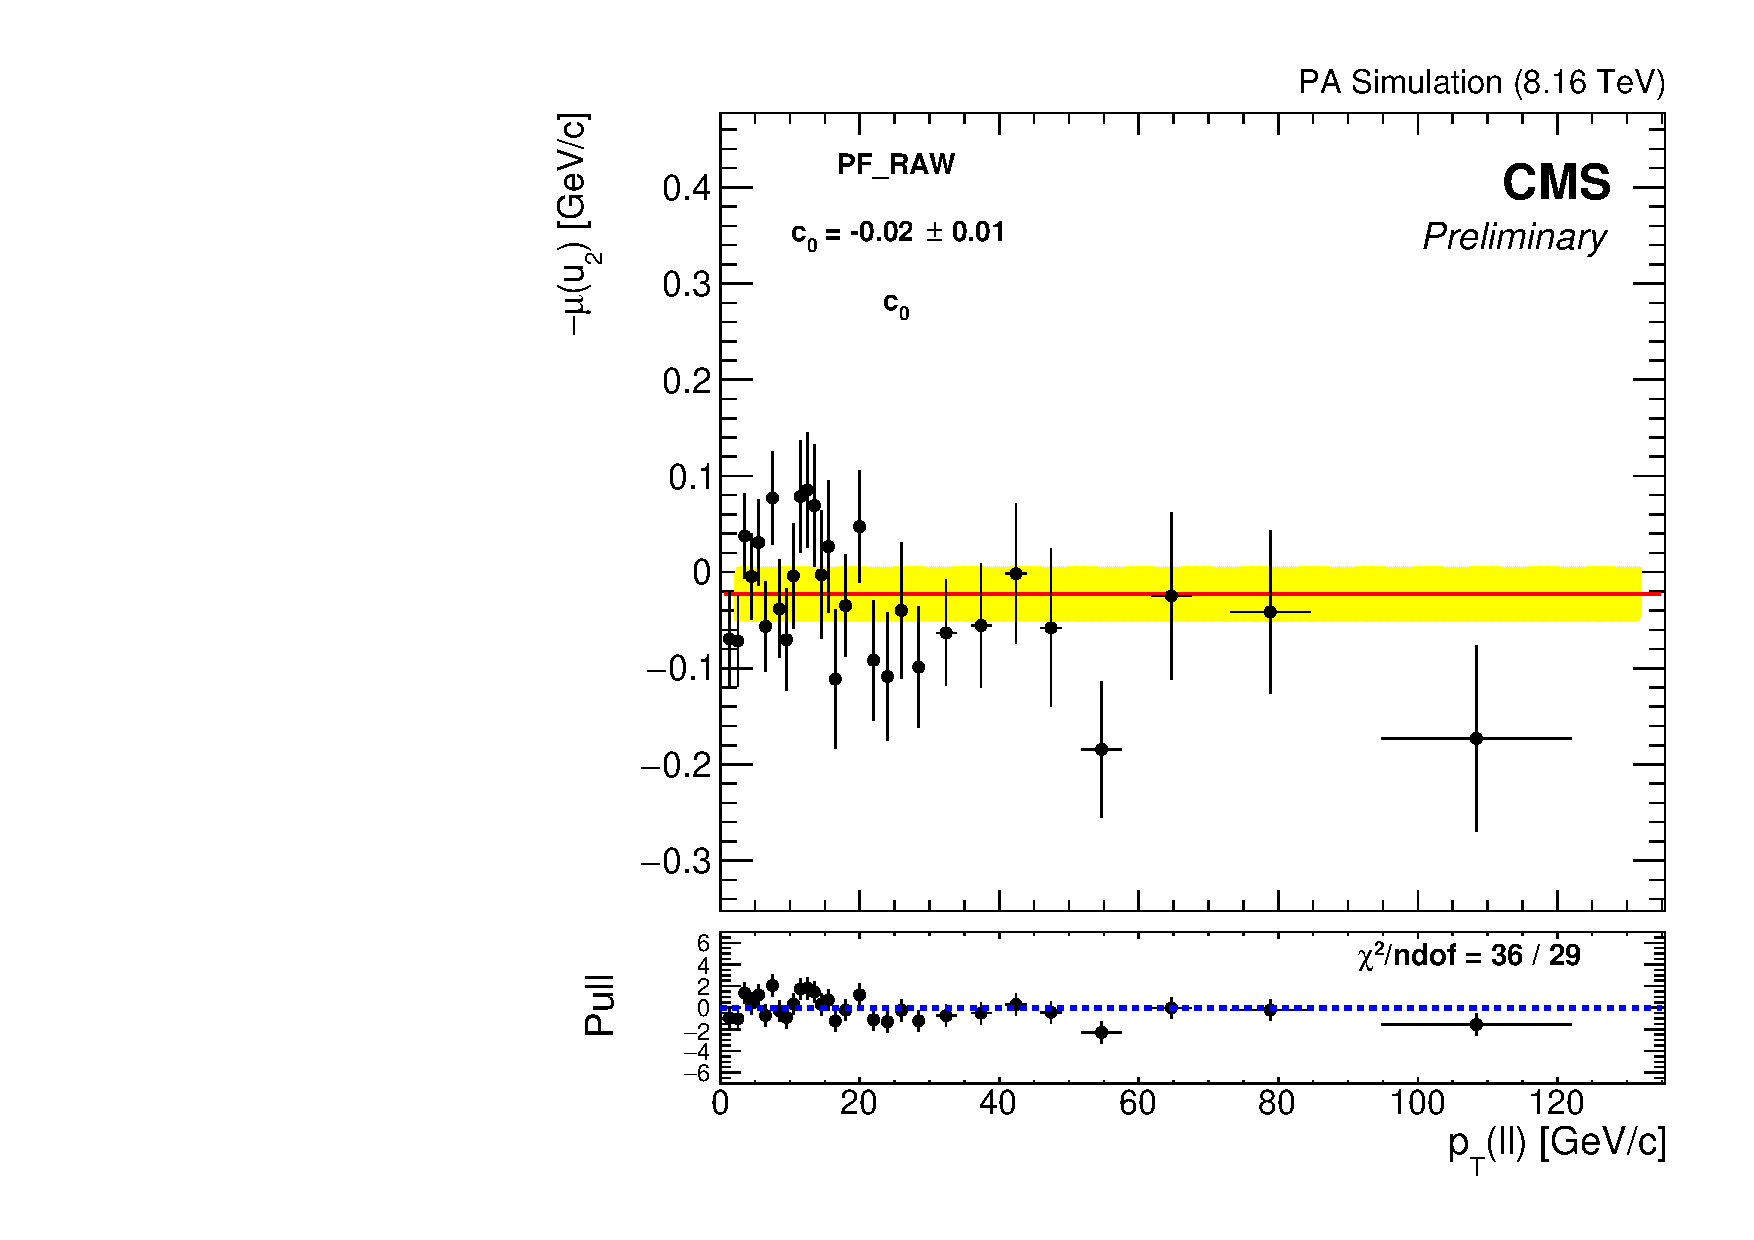
\includegraphics[width=0.45\textwidth]{Figures/WBoson/Analysis/Correction/Recoil/RecoilFitsqT/MC/fitPFu2mean.pdf}
 \caption{Fits of the profile of $\mu_{\perp}$ as a function of \qtZ. The results are derived from \ZToMuMu events in data (left) and simulation (right). The yellow band represents the 68\% error band of the fit.}
 \label{fig:figU2RecoilScaleFit}
\end{figure}

\paragraph{Parameterisation of the recoil resolution.} The two Gaussian width parameters ($\sigma_{\parallel(\perp),1}$ and $\sigma_{\parallel(\perp),2}$) of the parallel (perpendicular) component of the recoil are also extracted from the recoil fits for each \qtZ bin. The $\sigma_{\parallel(\perp),1}$ and $\sigma_{\parallel(\perp),2}$ parameters of \utpar (\utper) are parametrised as a function of \qtZ using the following formula:

\begin{equation}
 \sigma_{1,2}\left(\qtZ\right) = \sqrt{s_{0}^{2} + s_{1}^{2} \cdot q_{T}^{\alpha}}
 \label{eq:equreolnparam} 
\end{equation}

where $s_{0}$, $s_{1}$ and $\alpha$ are free parameters. The results of the fits to the $\sigma_{1}$ and $\sigma_{2}$ profiles as a function of \qtZ are presented in \fig{fig:figU1RecoilResolutionFit} for \utpar and in \fig{fig:figU2RecoilResolutionFit} for \utper. In addition, the profiles of the weighed average of the two Gaussian width parameters, given by:

\begin{equation}
 \begin{aligned}
  \sigma_{\perp} &= f_{\perp} \cdot \sigma_{\perp,1} + (1 - f_{\perp}) \cdot \sigma_{\perp,2} \\
  \sigma_{\parallel} &= f_{\parallel} \cdot \sigma_{\parallel,1} + (1 - f_{\parallel}) \cdot \sigma_{\parallel,2}
 \end{aligned}
 \label{eq:SigmaAvg} 
\end{equation}

are also fitted using \eq{eq:equreolnparam} and the results are shown in \fig{fig:figU2RecoilResolutionFit} and \fig{fig:figU1RecoilResolutionFit}.

\begin{figure}[htb!]
 \centering
 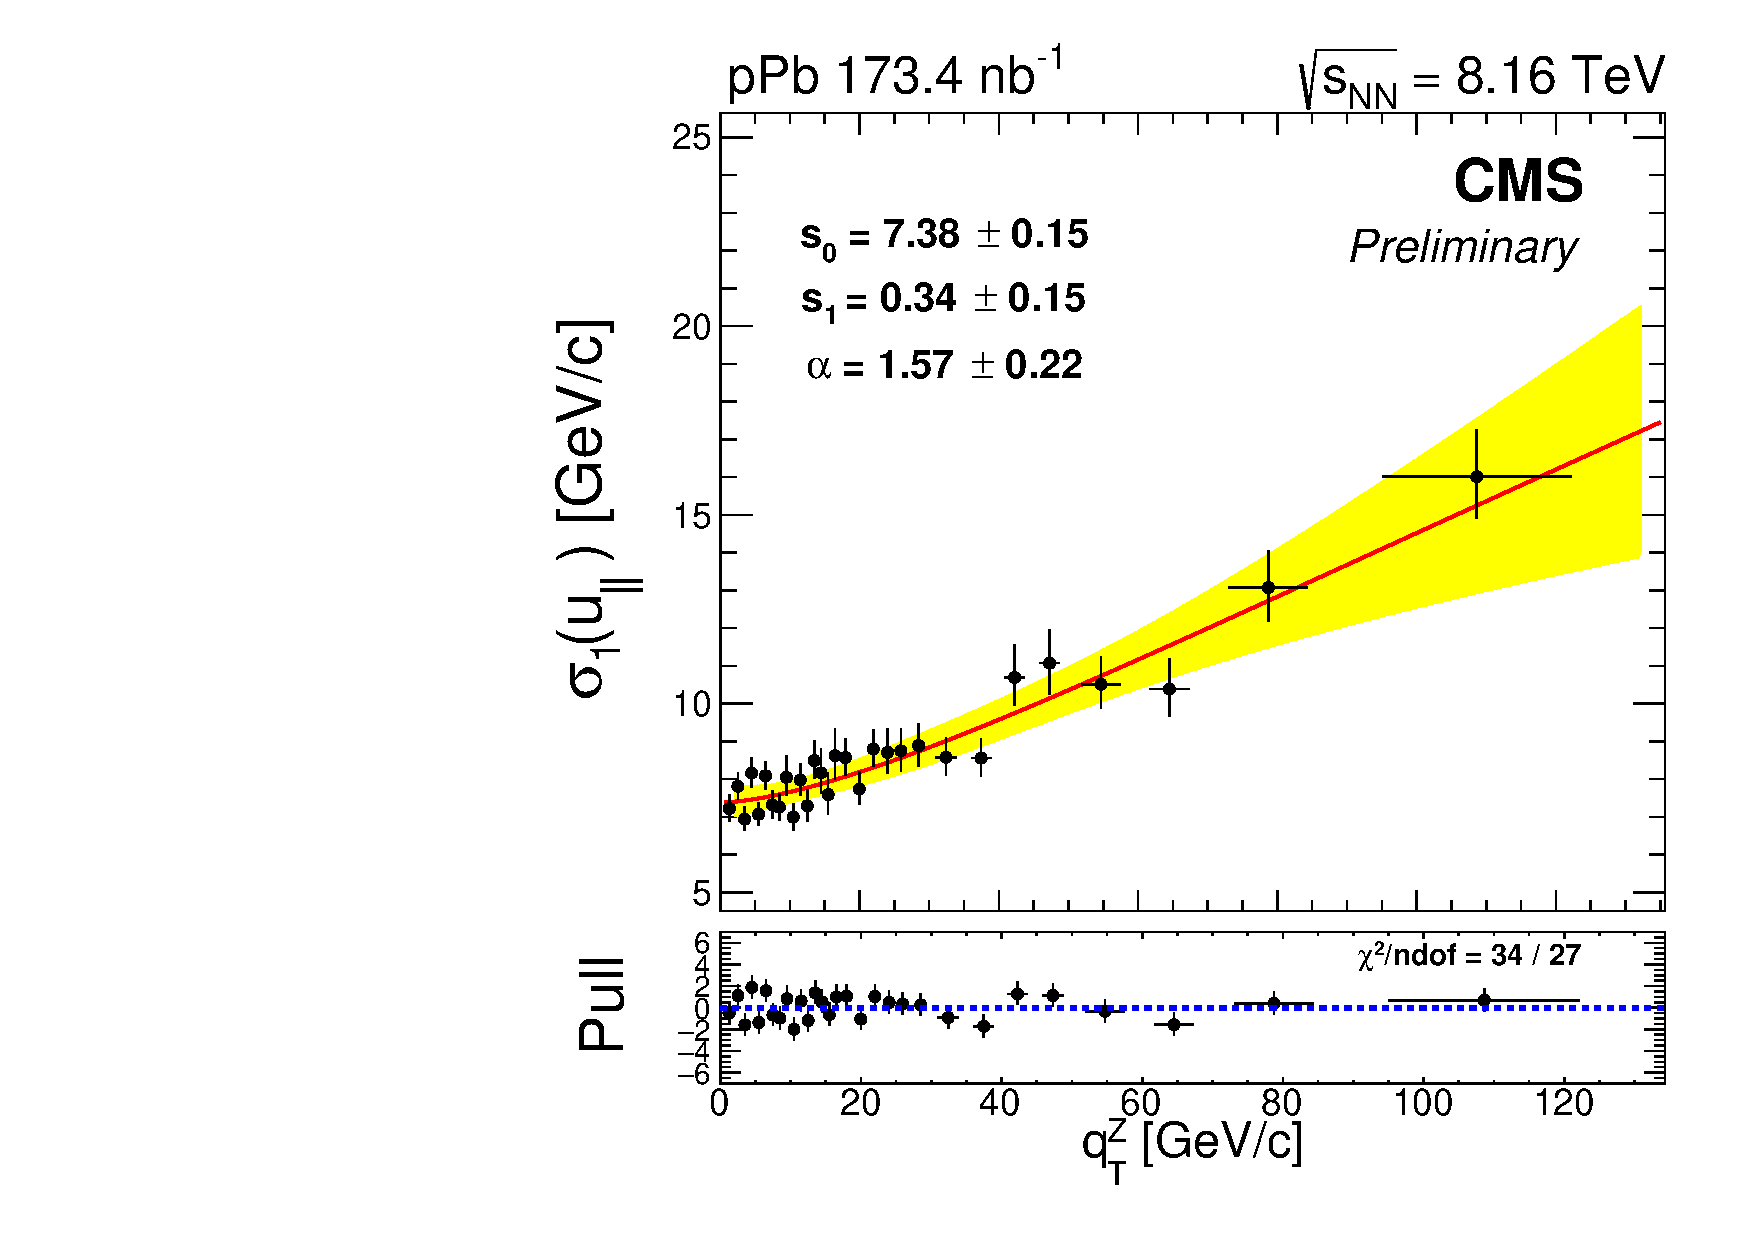
\includegraphics[width=0.3\textwidth]{Figures/WBoson/Analysis/Correction/Recoil/RecoilFitsqT/Data/fitPFu1sigma1.pdf}
 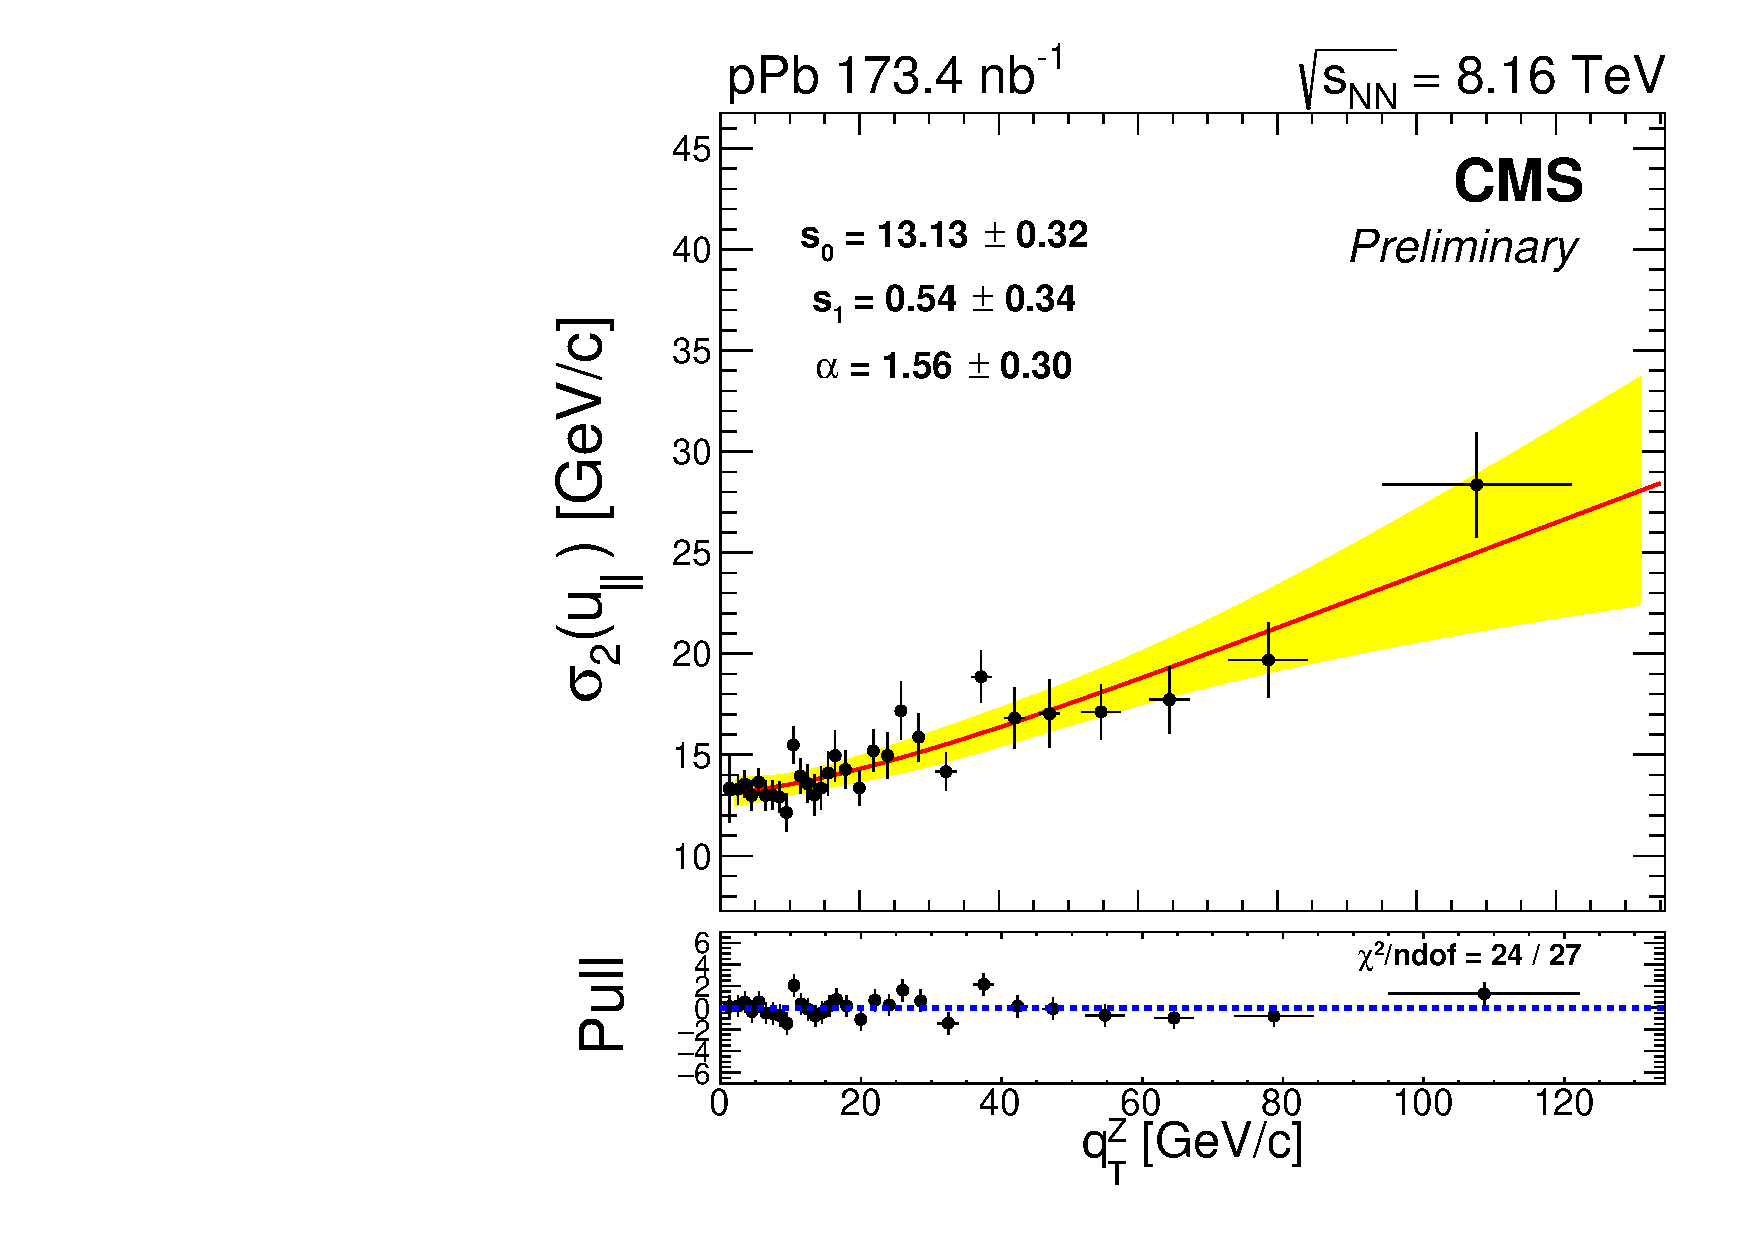
\includegraphics[width=0.3\textwidth]{Figures/WBoson/Analysis/Correction/Recoil/RecoilFitsqT/Data/fitPFu1sigma2.pdf}
 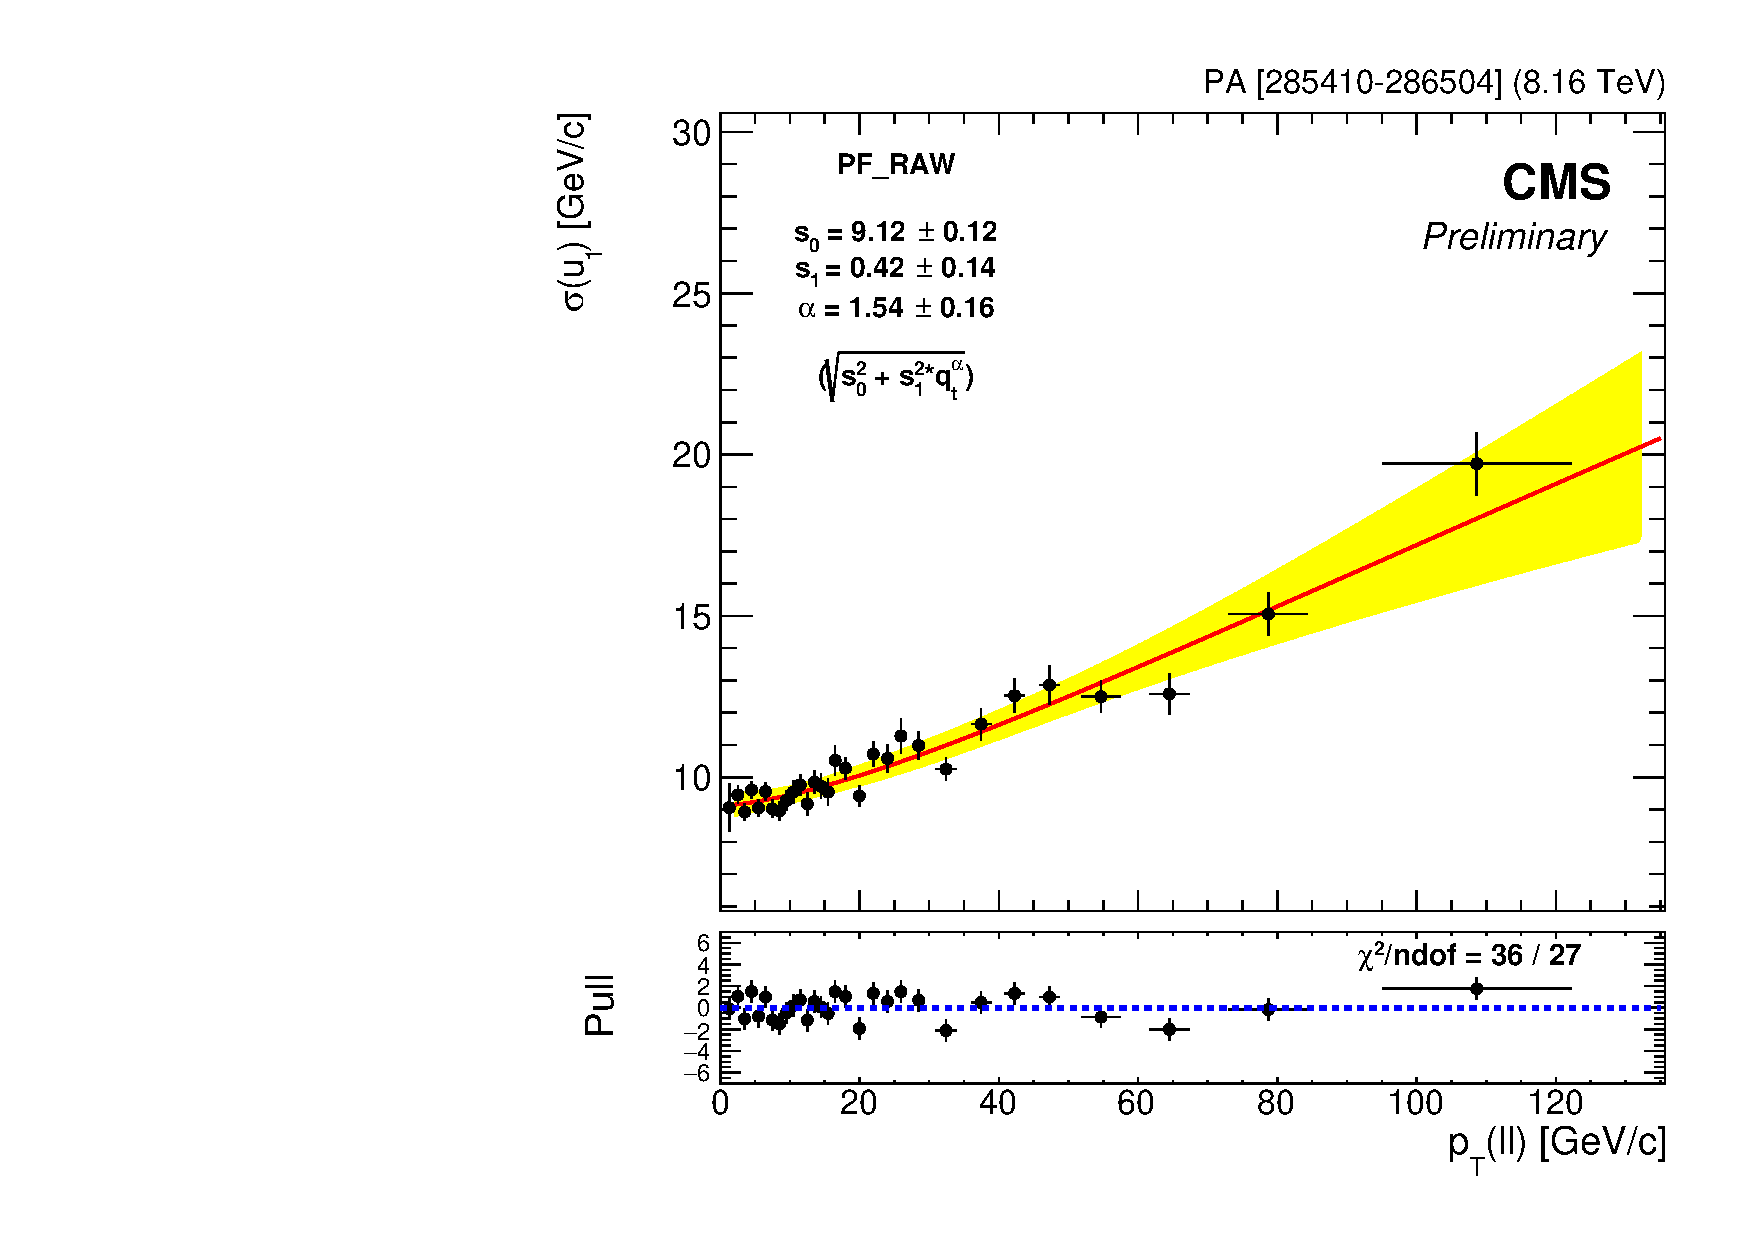
\includegraphics[width=0.3\textwidth]{Figures/WBoson/Analysis/Correction/Recoil/RecoilFitsqT/Data/fitPFu1sigma.pdf} \\
 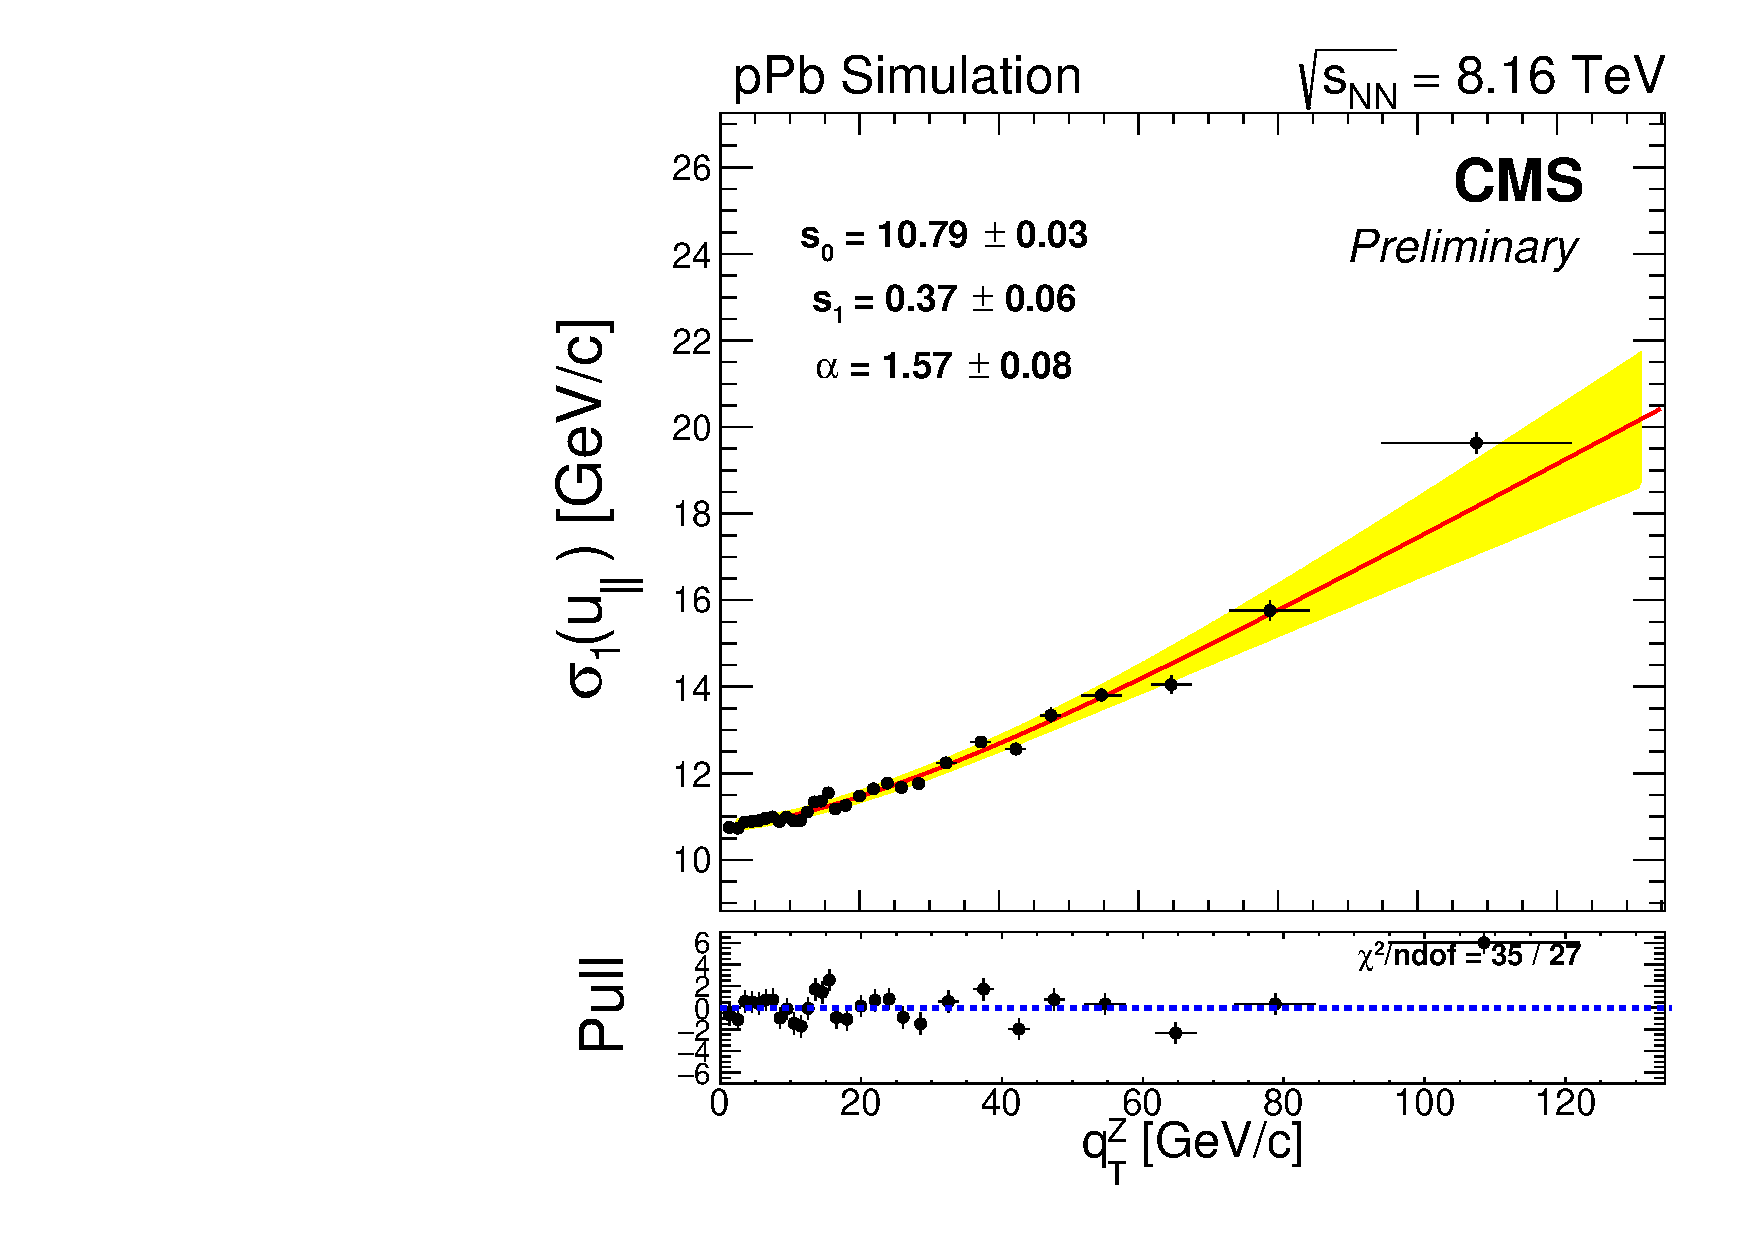
\includegraphics[width=0.3\textwidth]{Figures/WBoson/Analysis/Correction/Recoil/RecoilFitsqT/MC/fitPFu1sigma1.pdf}
 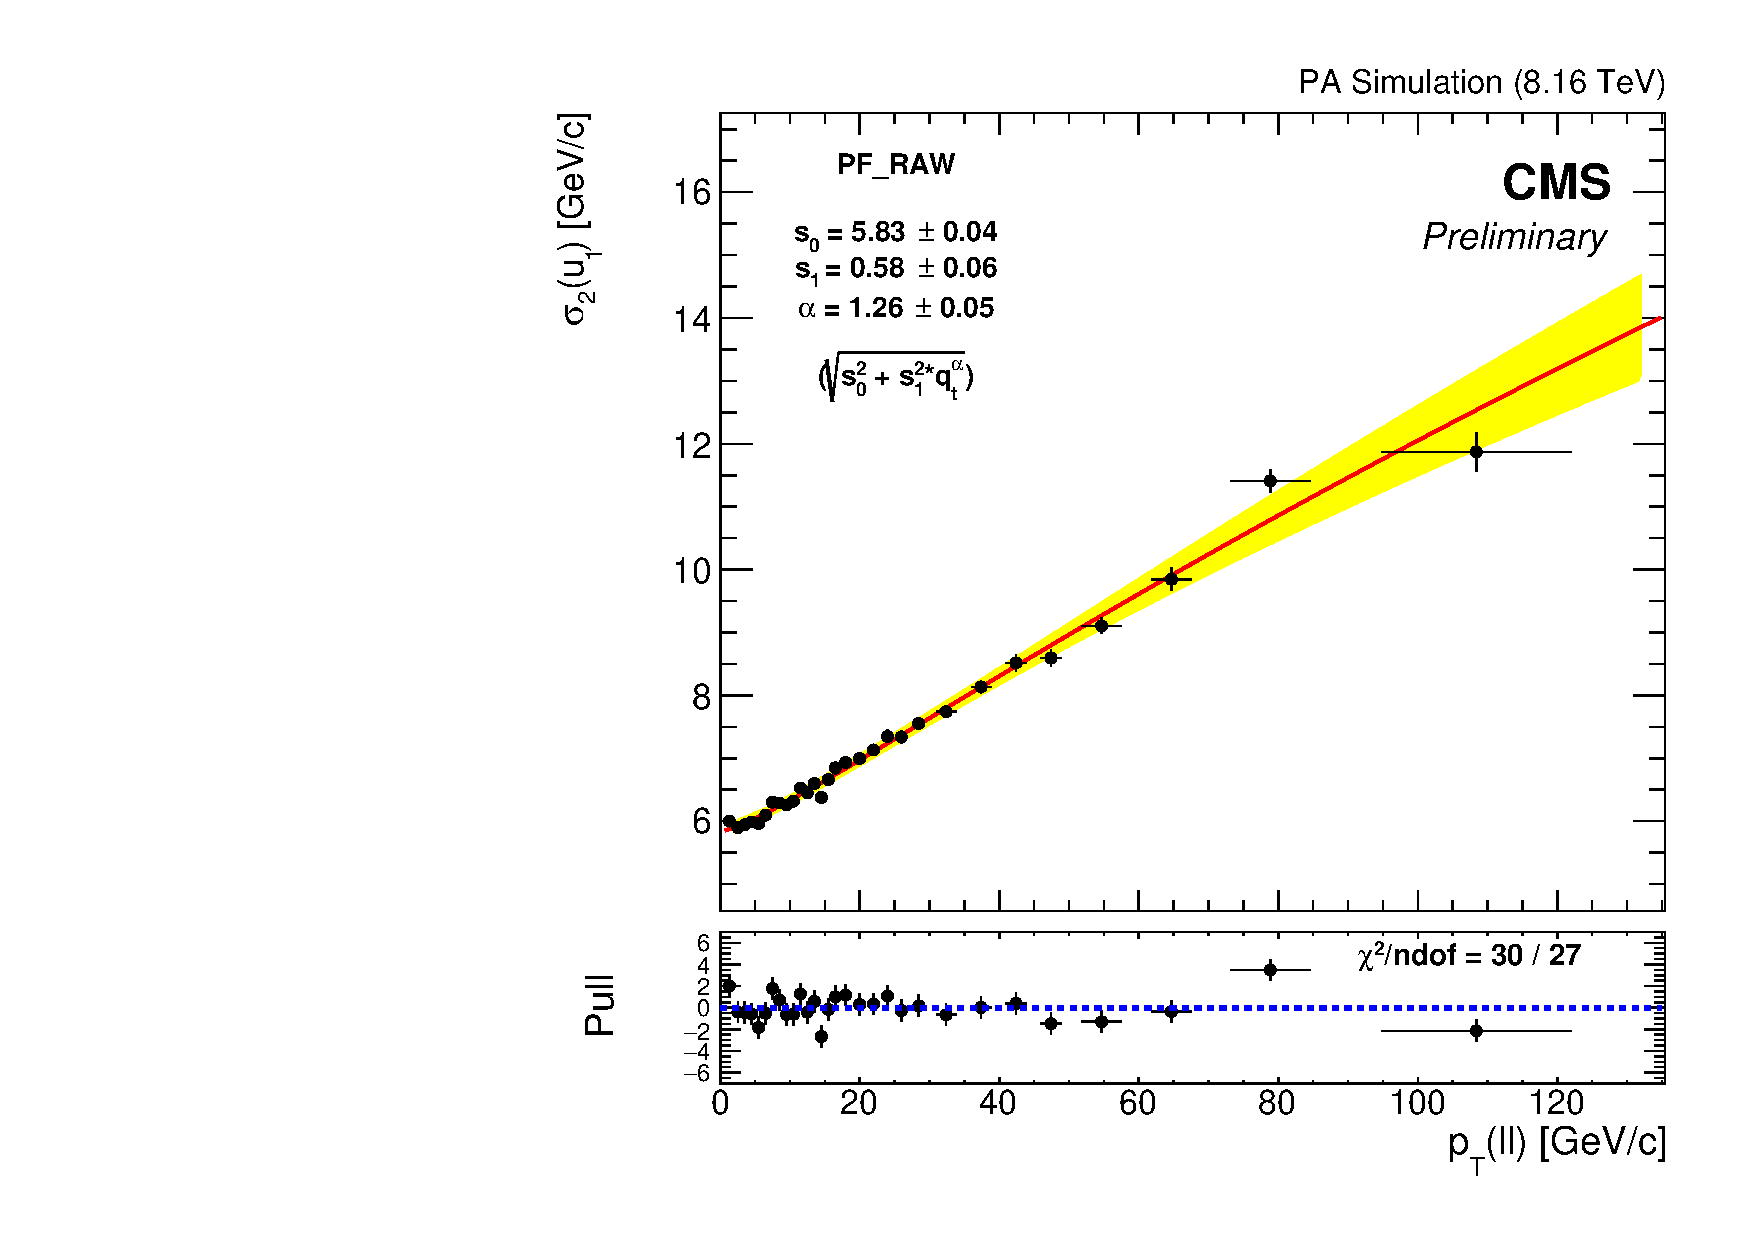
\includegraphics[width=0.3\textwidth]{Figures/WBoson/Analysis/Correction/Recoil/RecoilFitsqT/MC/fitPFu1sigma2.pdf}
 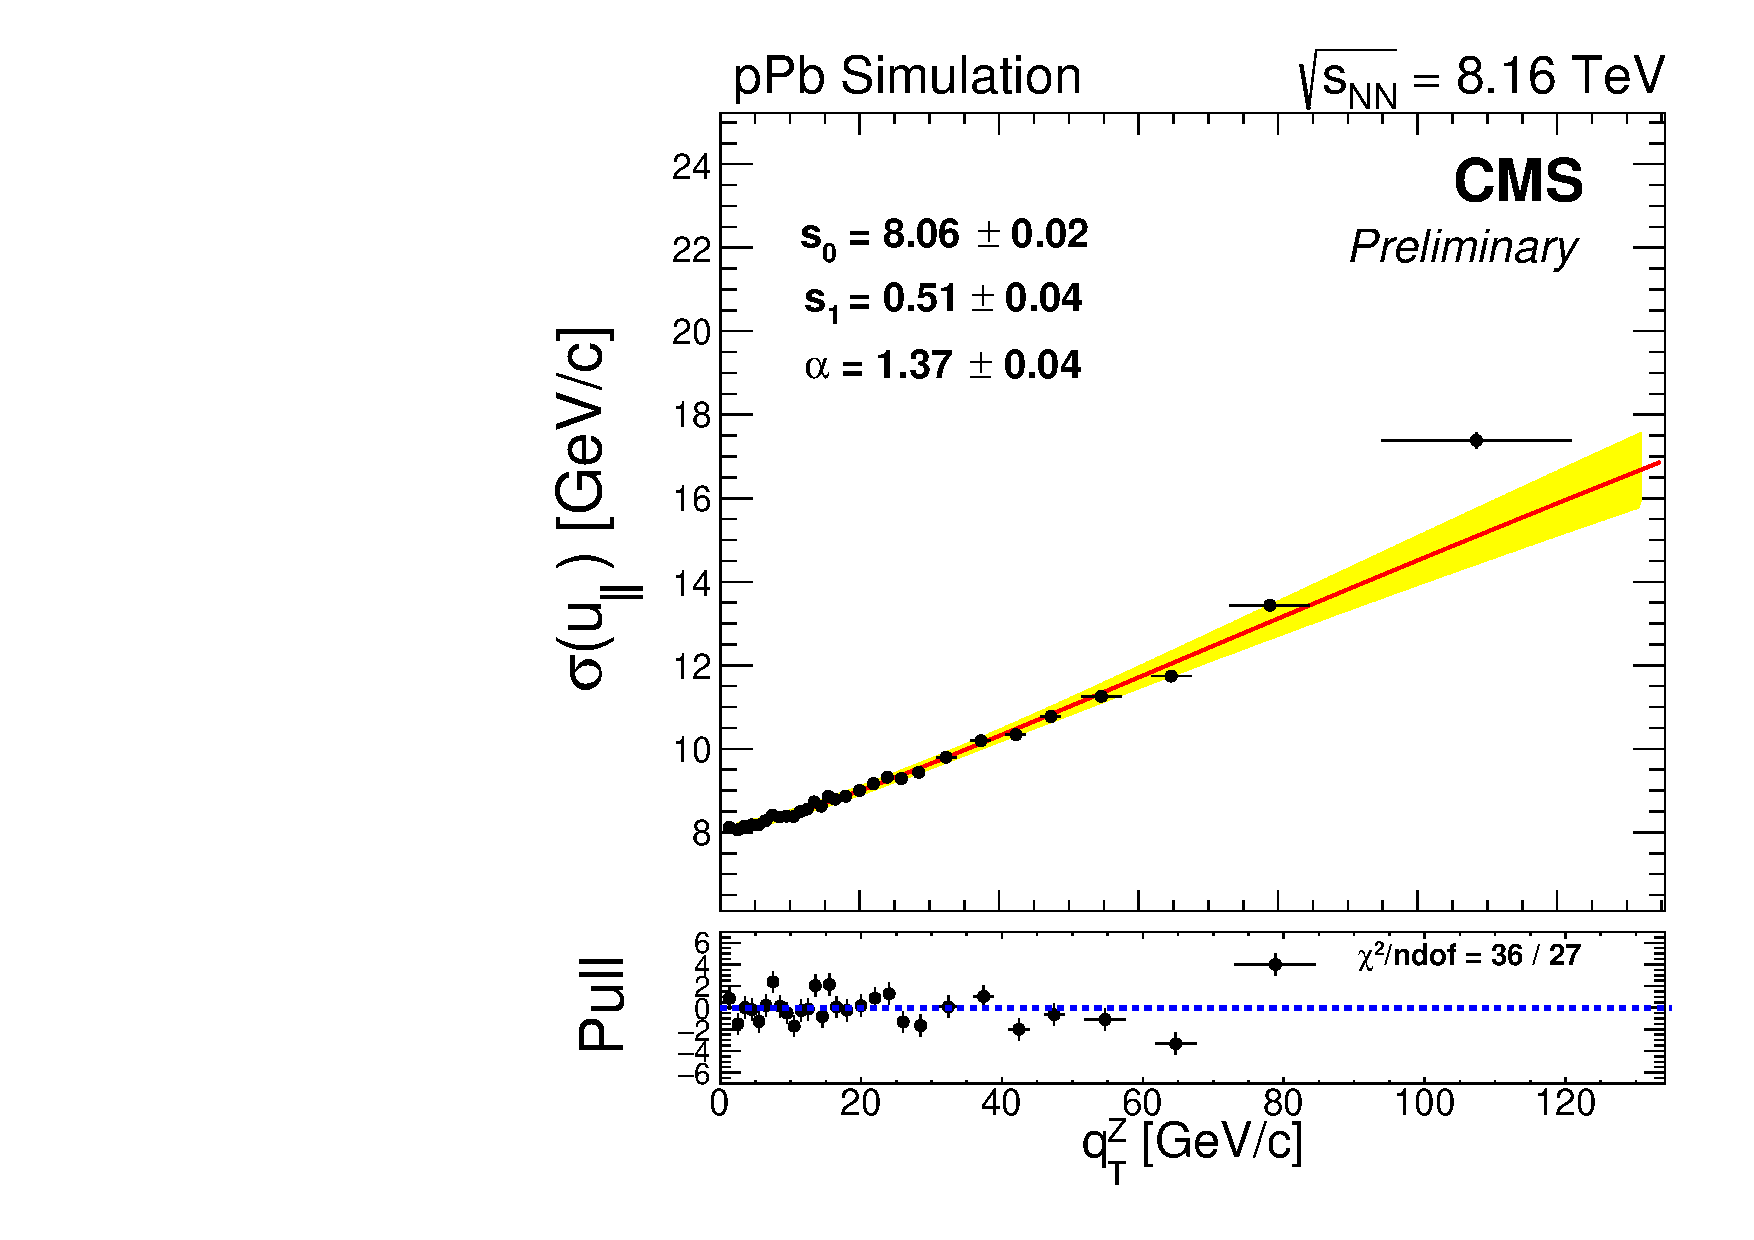
\includegraphics[width=0.3\textwidth]{Figures/WBoson/Analysis/Correction/Recoil/RecoilFitsqT/MC/fitPFu1sigma.pdf}
 \caption{Fits to the profile of the $\sigma_{\parallel,1}$ (left), $\sigma_{\parallel,2}$ (middle) and weighed average $\sigma_{\parallel}$ (right) values of the parallel recoil component as a function of \qtZ. . The results are derived from \ZToMuMu events in data (top) and simulation (bottom).}
 \label{fig:figU1RecoilResolutionFit}
\end{figure}

\begin{figure}[htb!]
 \centering
 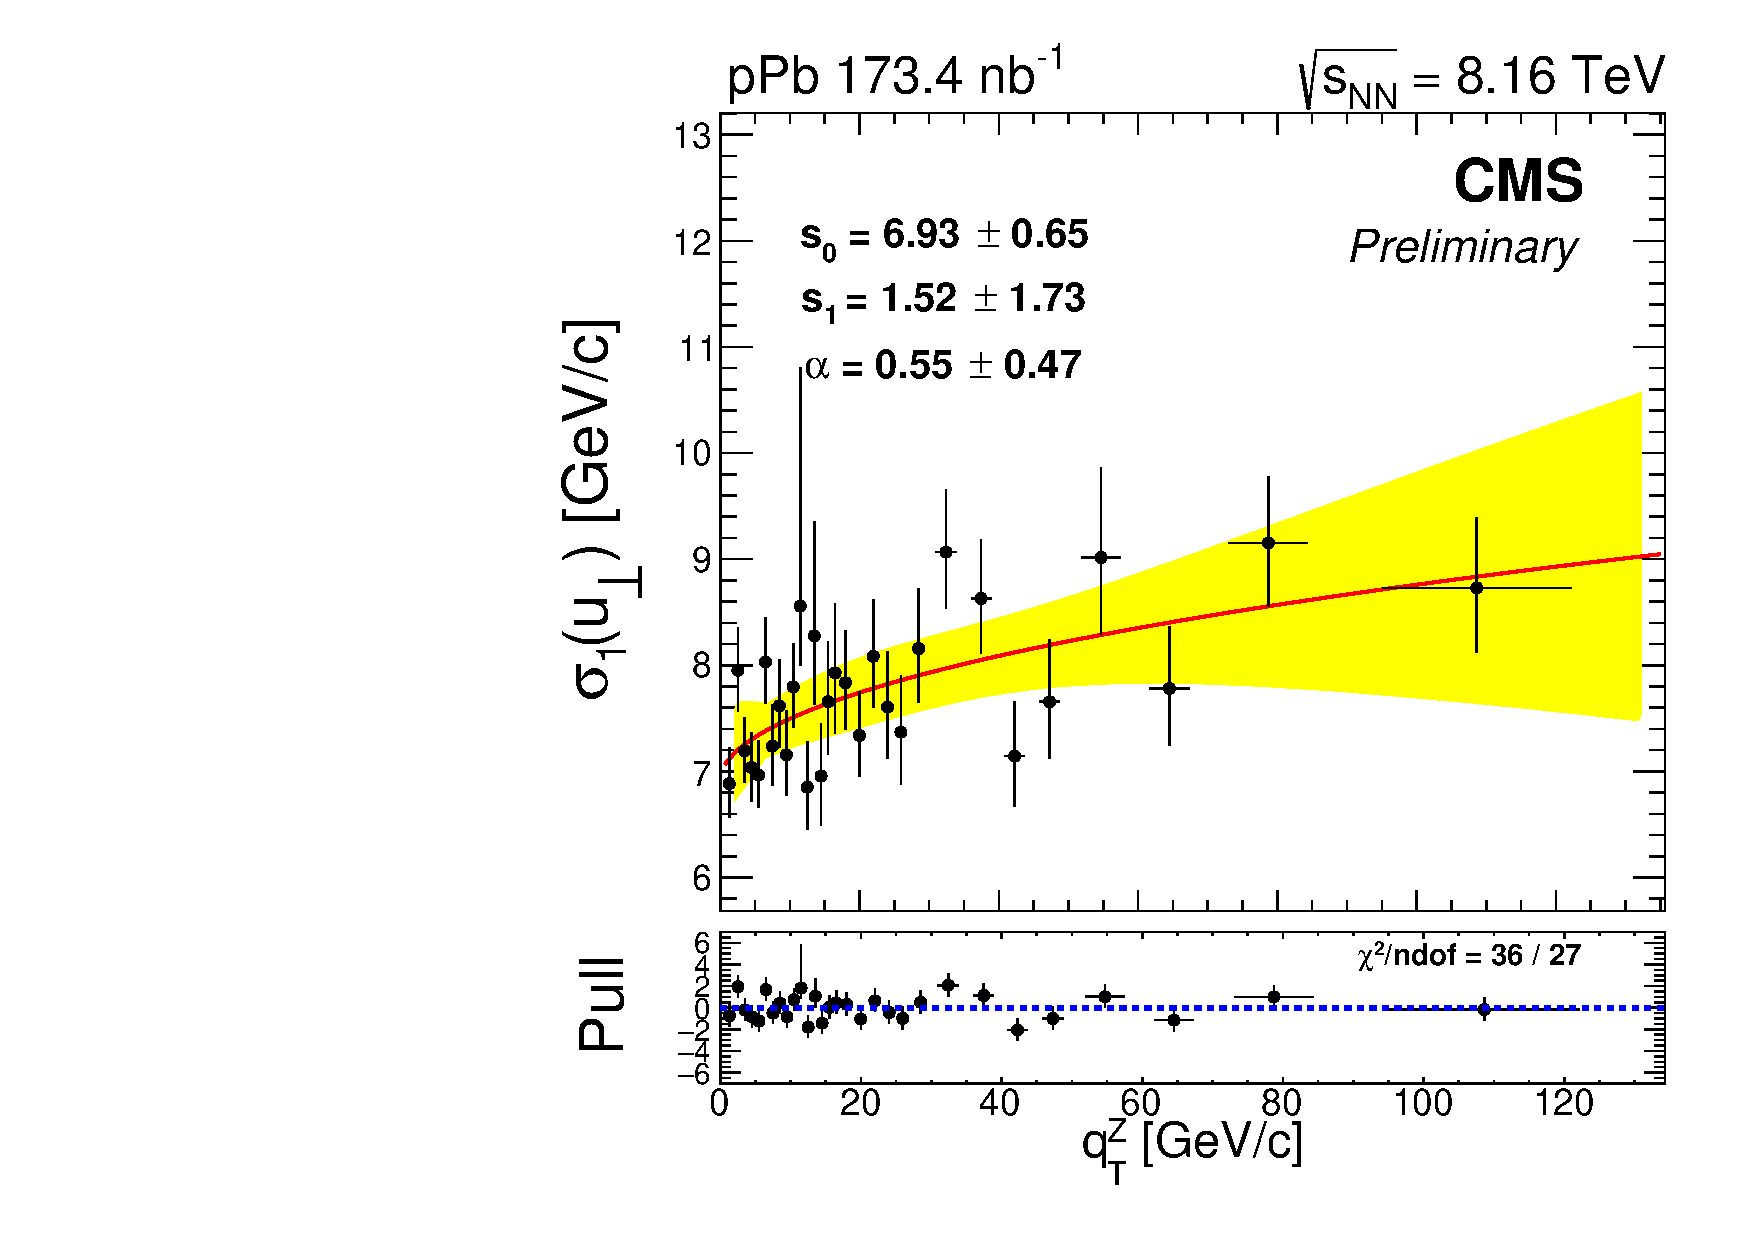
\includegraphics[width=0.3\textwidth]{Figures/WBoson/Analysis/Correction/Recoil/RecoilFitsqT/Data/fitPFu2sigma1.pdf}
 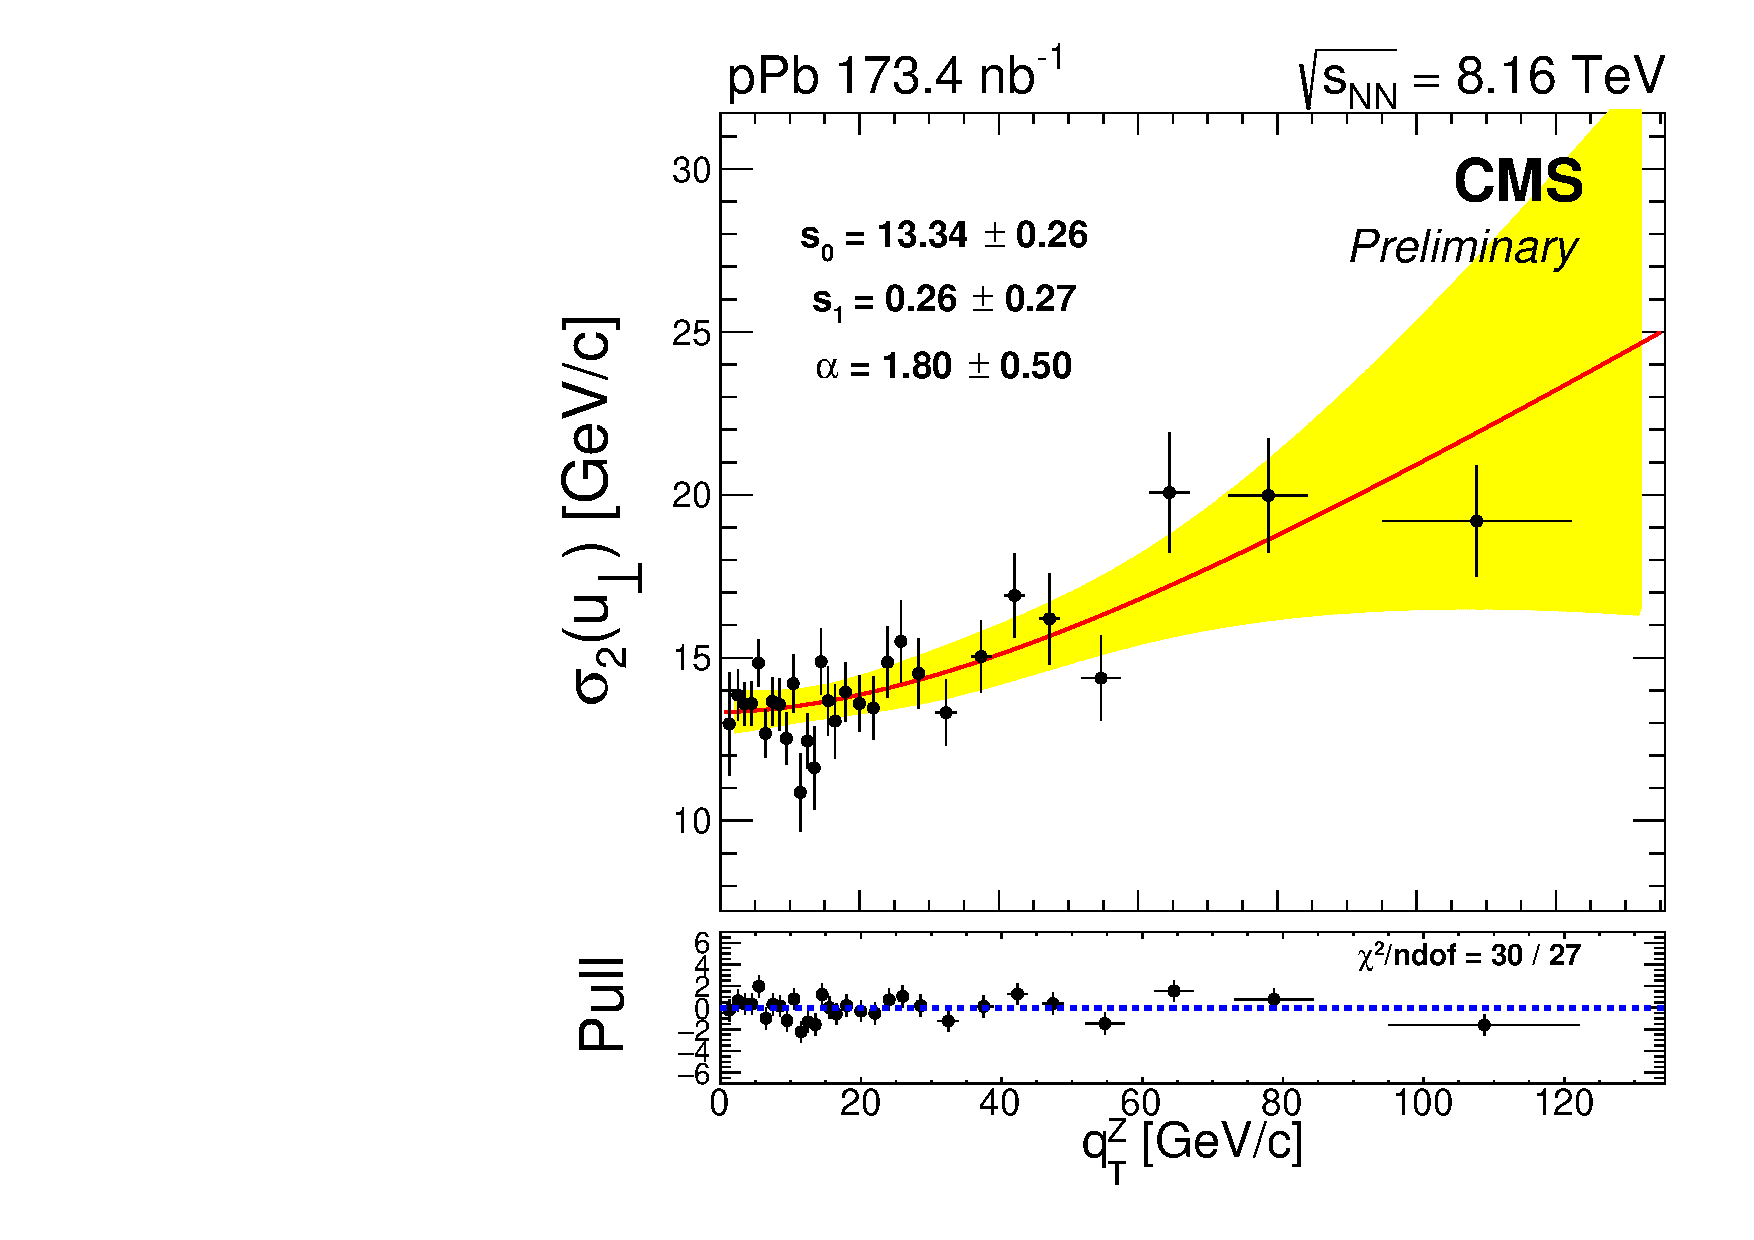
\includegraphics[width=0.3\textwidth]{Figures/WBoson/Analysis/Correction/Recoil/RecoilFitsqT/Data/fitPFu2sigma2.pdf}
 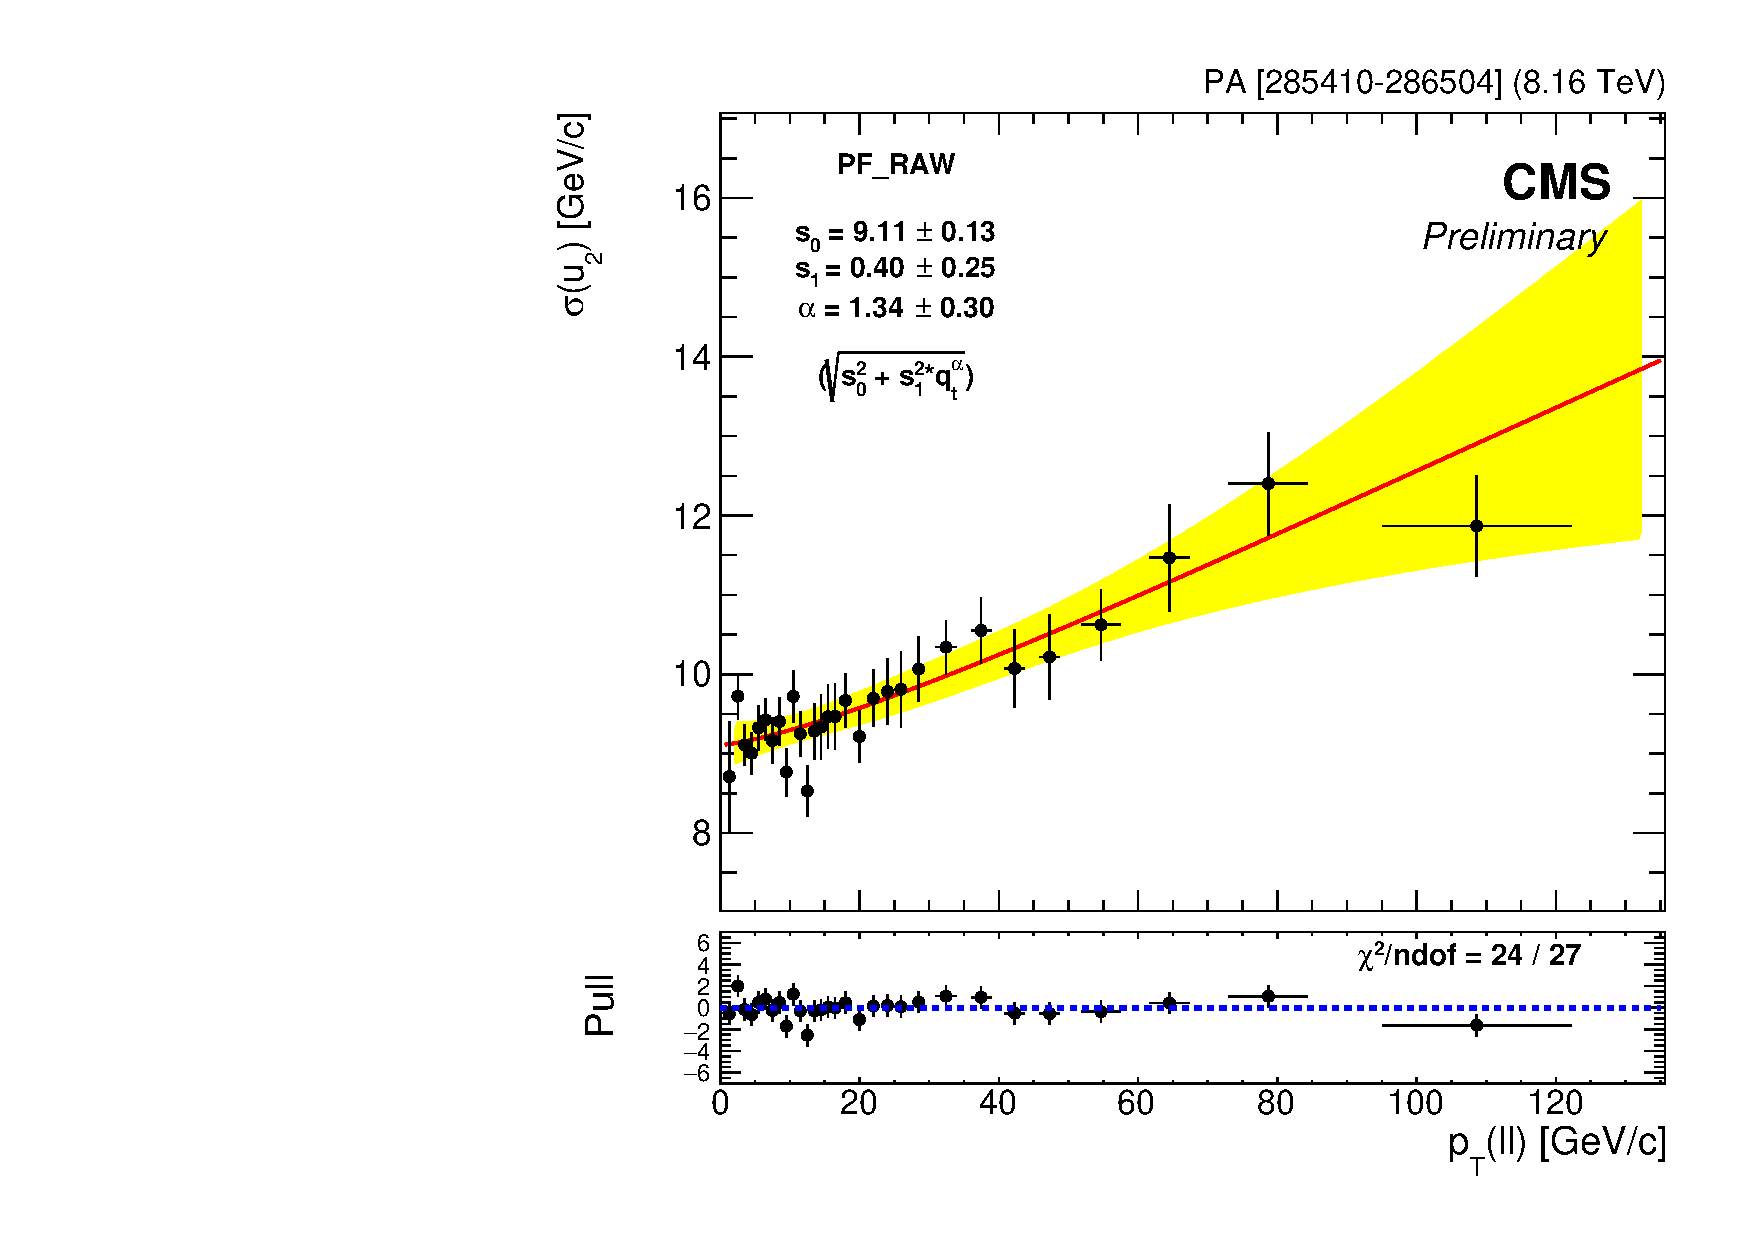
\includegraphics[width=0.3\textwidth]{Figures/WBoson/Analysis/Correction/Recoil/RecoilFitsqT/Data/fitPFu2sigma.pdf} \\
 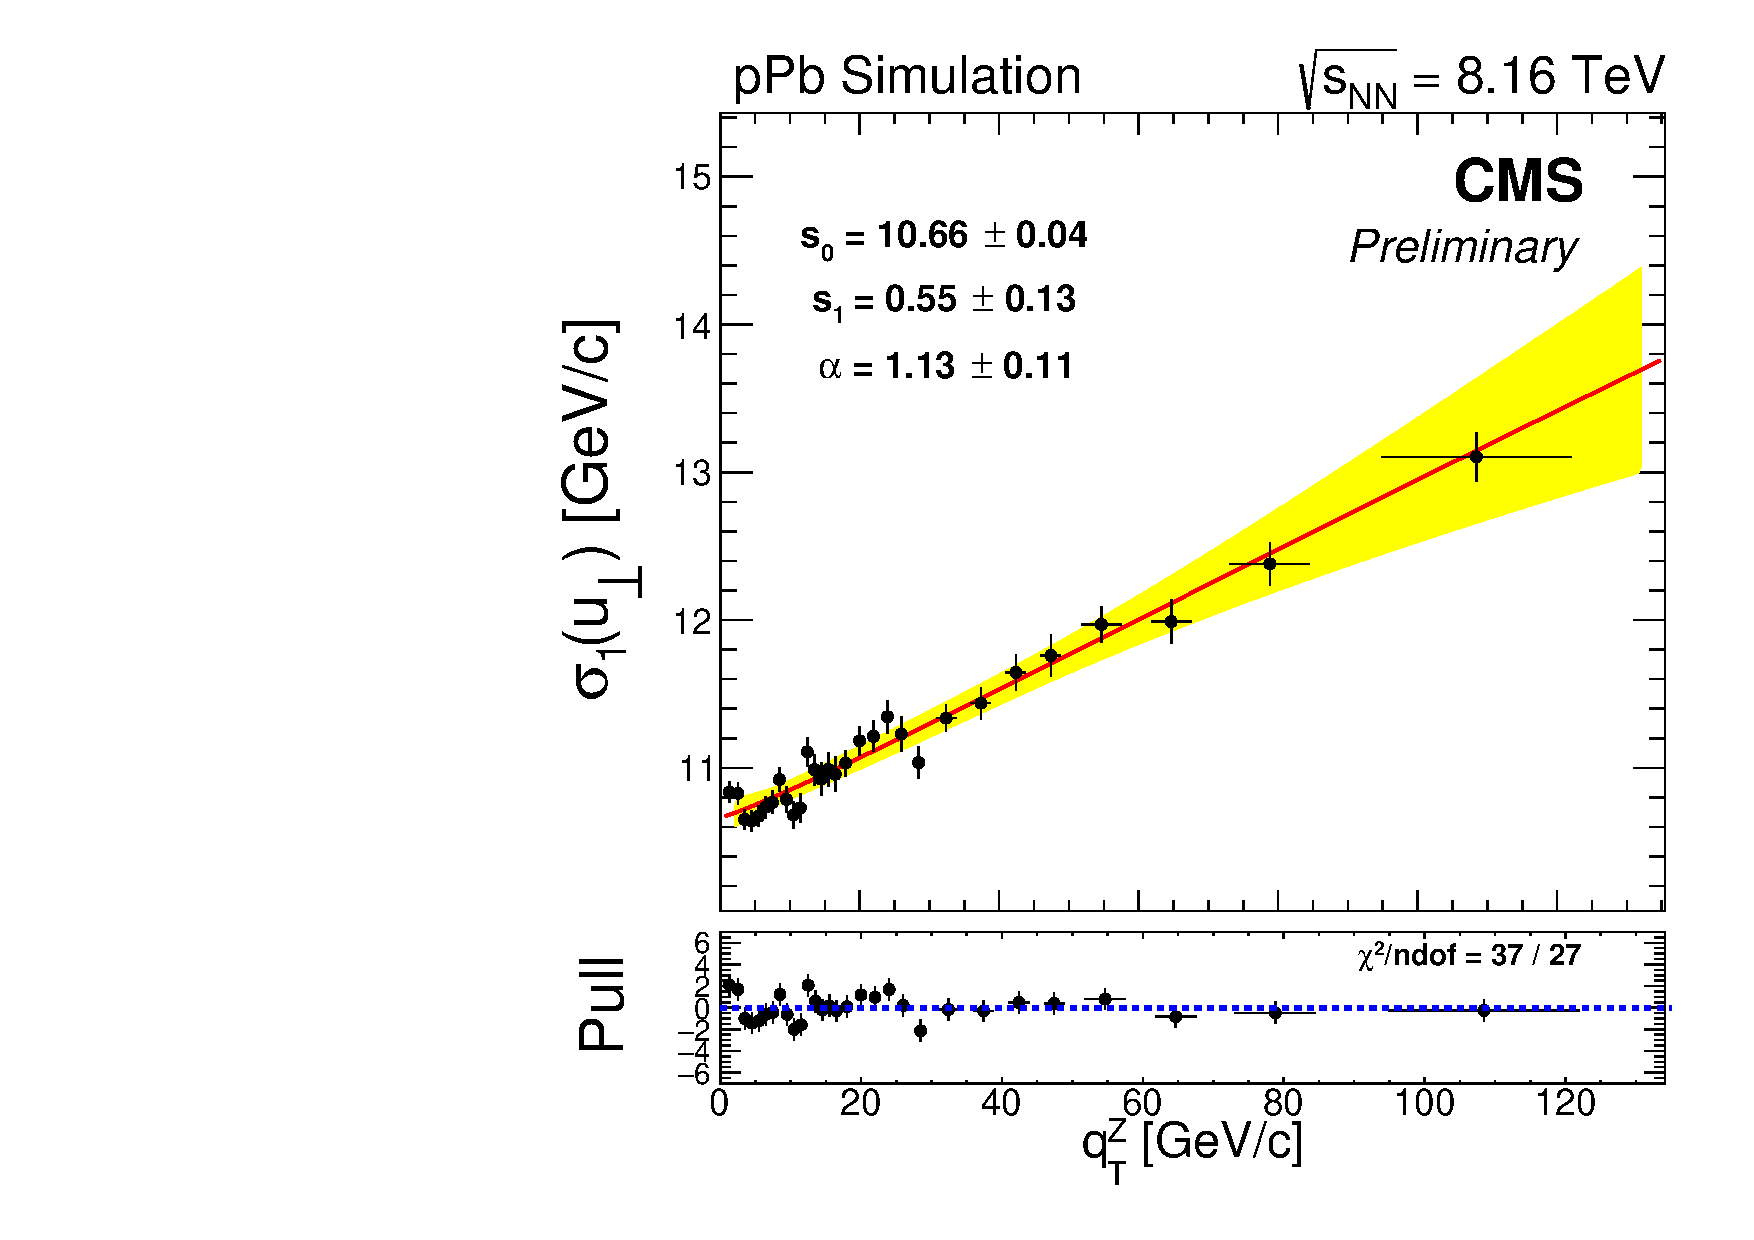
\includegraphics[width=0.3\textwidth]{Figures/WBoson/Analysis/Correction/Recoil/RecoilFitsqT/MC/fitPFu2sigma1.pdf}
 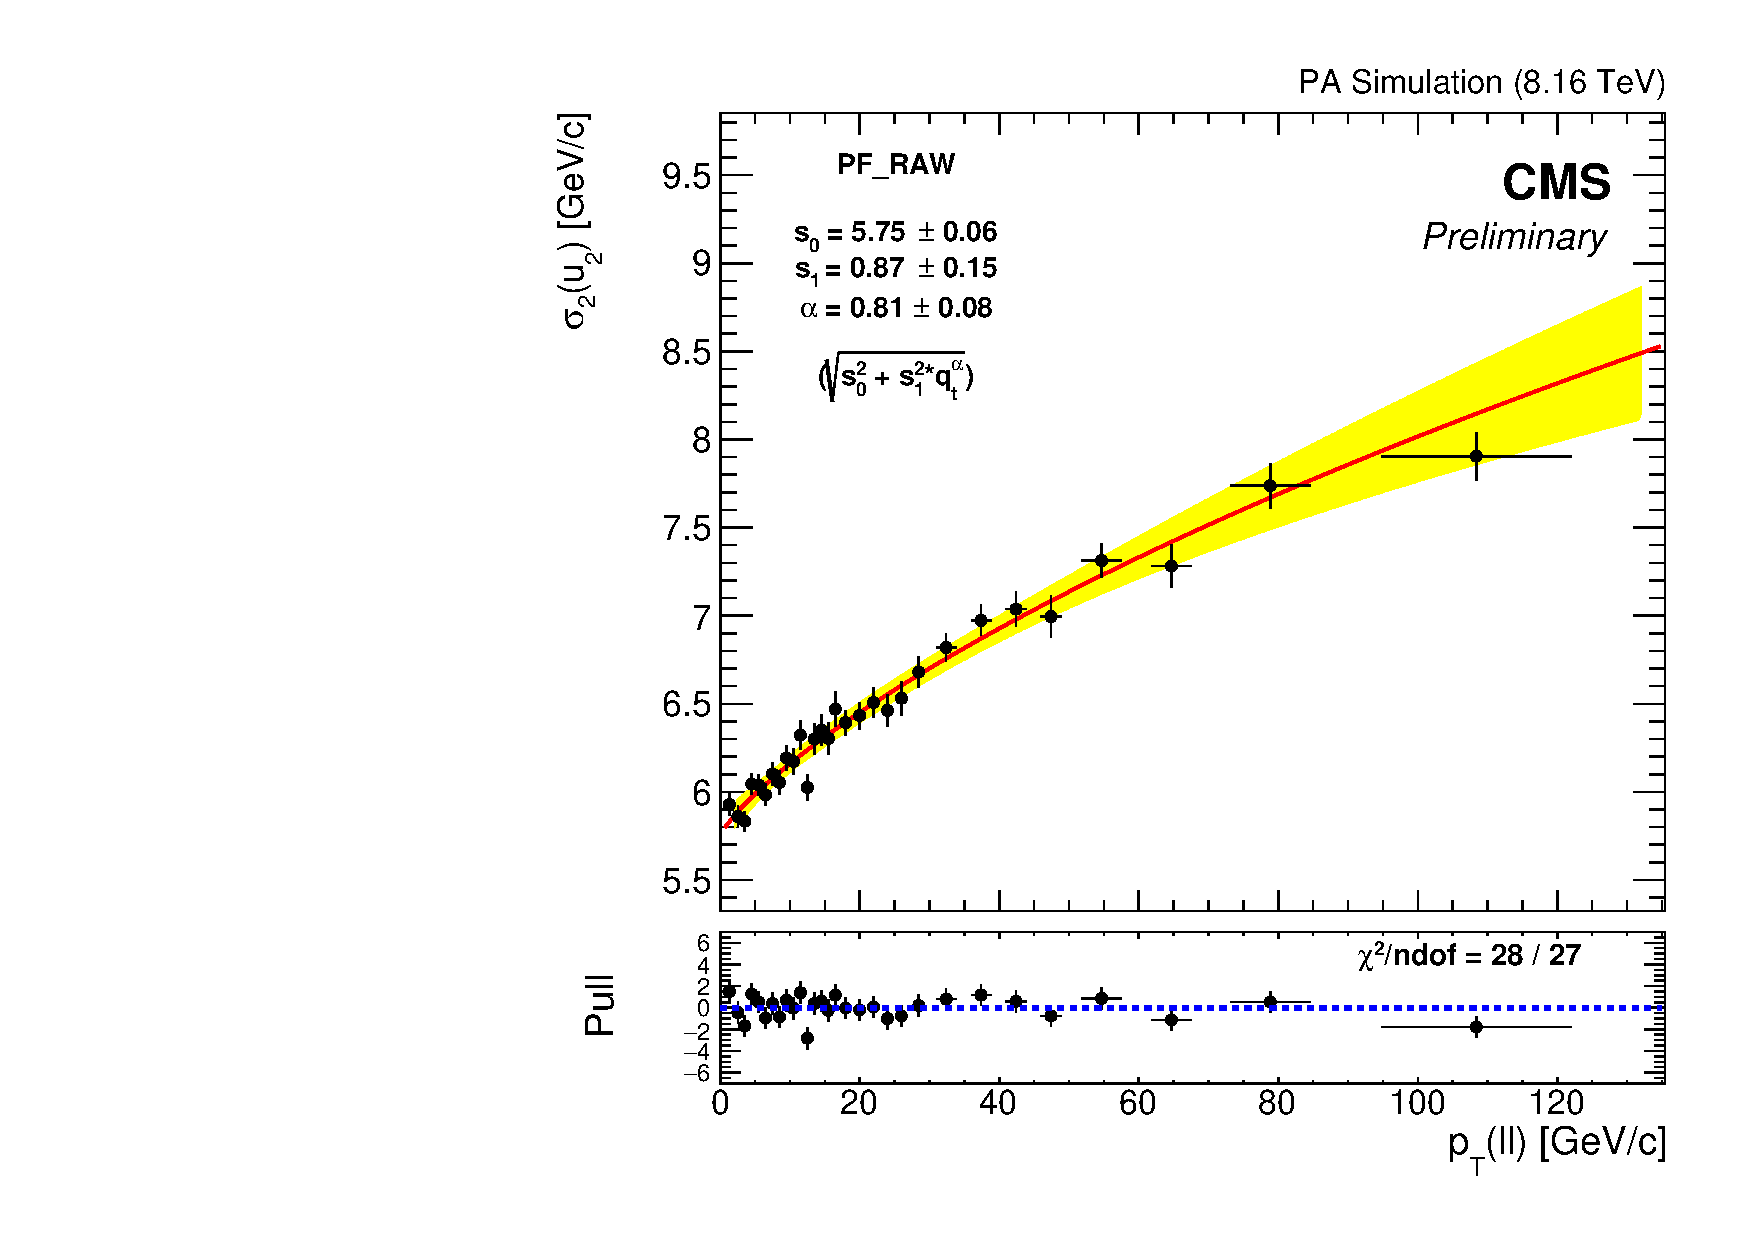
\includegraphics[width=0.3\textwidth]{Figures/WBoson/Analysis/Correction/Recoil/RecoilFitsqT/MC/fitPFu2sigma2.pdf}
 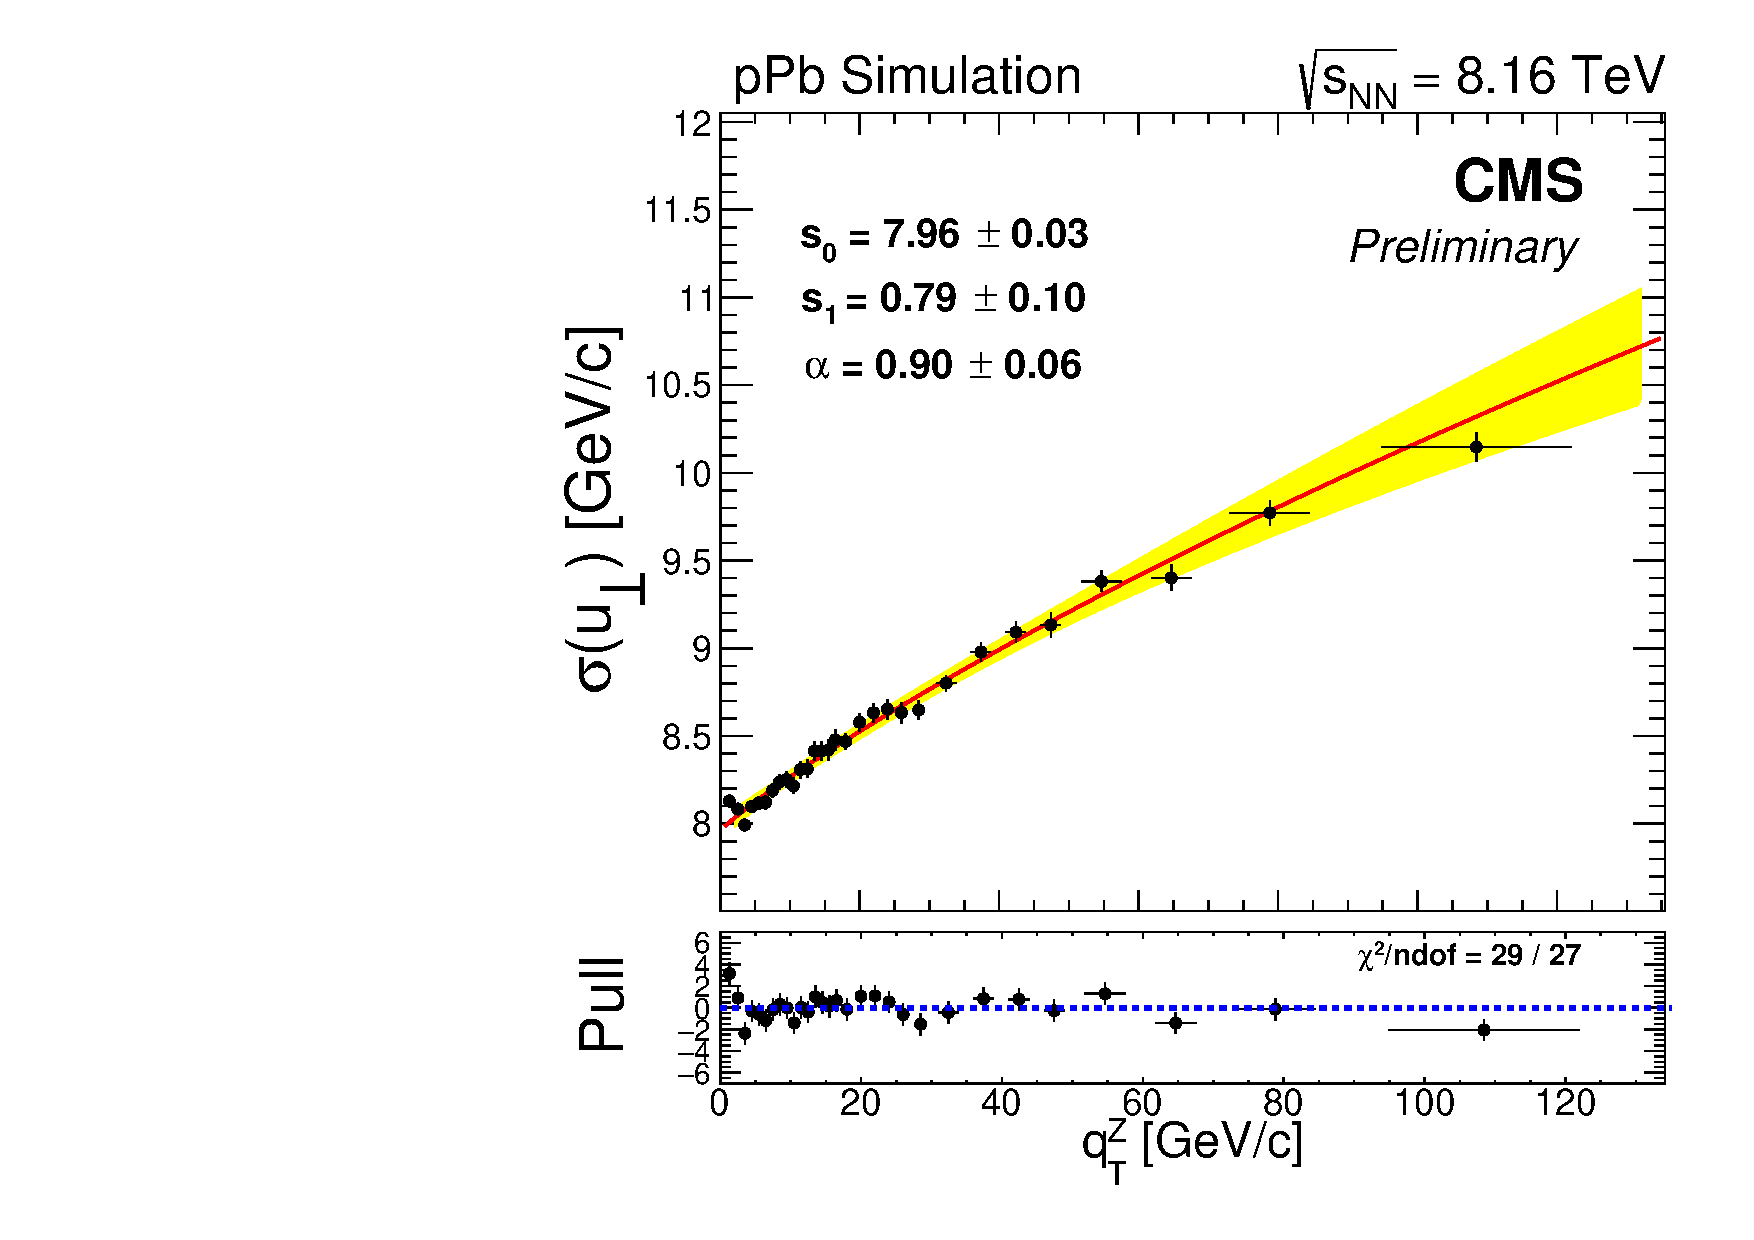
\includegraphics[width=0.3\textwidth]{Figures/WBoson/Analysis/Correction/Recoil/RecoilFitsqT/MC/fitPFu2sigma.pdf}
 \caption{Fits for the $\sigma_{\perp,1}$ (left), $\sigma_{\perp,2}$ (middle) and weighed average $\sigma_{\perp}$ (right) values of the recoil perpendicular component as a function of $q_{T}$. The results are derived from \ZToMuMu events in data (top) and simulation (bottom).}
 \label{fig:figU2RecoilResolutionFit}
\end{figure}

It is observed in \fig{fig:figU1RecoilResolutionFit} and \ref{fig:figU2RecoilResolutionFit}, that the recoil resolution increases with \qtZ. This is expected since high-\pt \Z bosons are produced in association with several jets from higher order processes, which contributes to the recoil resolution. 

Also, the parameter $s_{0}$ of the weighed average $\sigma$, which measure the recoil resolution at $\qtZ = 0~\GeVc$, is found to be larger in data than in simulation, which means that the modelling of the contributions not originating from the hard scattering (e.g. underlying events) are underestimated compared to data. In addition, the contributions to the recoil resolution at high \qtZ are also larger in data than in simulation.

\paragraph{Calibration of the simulated recoil.} The recoil corrections are applied to the following simulated processes: \WToMuNu, \DYToMuMu and \WToTauNu. The simulated recoil distribution is calibrated using the parametric equations obtained in the previous sections for the Gaussian mean $\mu(\qt)$ and weighed-average  width $\sigma(\qt)$. These parametric equations are summarised below:
\begin{itemize}
  \item Recoil parametric equations from data: 
\begin{equation}
 \begin{aligned}
  \mu^{\text{data}}_{\parallel}\left(\qt\right) &= \left(0.5 + 0.9{\cdot}\qt\right)\left(\frac{1 + \text{Erf}\left[0.1{\cdot}\left(\qt\right)^{0.7}\right]}{2}\right) \\
  \sigma^{\text{data}}_{\parallel}\left(\qt\right) &= \sqrt{9.1^{2} + 0.4^{2}{\cdot}\left(\qt\right)^{1.5}} \\
  \sigma^{\text{data}}_{\perp}\left(\qt\right) &= \sqrt{9.1^{2} + 0.4^{2}{\cdot}\left(\qt\right)^{1.3}}
 \end{aligned}
\end{equation}
  \item Recoil parametric equations from simulation:
\begin{equation}
 \begin{aligned}
  \mu^{\text{MC}}_{\parallel}\left(\qt\right) &= \left(0.1 + 0.9{\cdot}\qt\right)\left(\frac{1 + \text{Erf}\left[0.2{\cdot}\left(\qt\right)^{0.5}\right]}{2}\right) \\
  \sigma^{\text{MC}}_{\parallel}\left(\qt\right) &= \sqrt{8.1^{2} + 0.5^{2}{\cdot}\left(\qt\right)^{1.4}} \\
  \sigma^{\text{MC}}_{\perp}\left(\qt\right) &= \sqrt{8.0^{2} + 0.8^{2}{\cdot}\left(\qt\right)^{0.9}}
 \end{aligned}
\end{equation}
\end{itemize}

The procedure to calibrate the simulated recoil starts by computing the \pt vector of the boson (\qtvec) and simulated recoil ($\utvec^{\text{MC}}$). The boson \qtvec is determined using the reconstructed muon information whenever possible, as described below:
\begin{itemize}
 \item \WToMuNu: \qtvec is the \ptvec sum of the reconstructed muon and generated neutrino.
 \item \WToTauNu: \qtvec is the generated \Wb boson \pt vector.
 \item \DYToMuMu: if one of the muons is not reconstructed, then \qtvec is the \ptvec sum of the reconstructed  muon and the generated-only muon, otherwise \qtvec is equal to the \ptvec sum of both reconstructed muons ($\qtvec^{\DY}$).
\end{itemize}

The recoil $\utvec^{\text{MC}}$ of the simulated event is derived by \textit{removing} from the \ptvecmiss, the reconstructed muons from the decay of the weak boson. In other words, for \WToMuNu events, $\DYToMuMu$ events with only one reconstructed muon ($\DY\to\mu$) and \WToTauNu events, the $\utvec^{\text{MC}} = -\ptvecmiss - \ptMuvec$, while for \DYToMuMu events with both muons reconstructed, the $\utvec^{\text{MC}} = -\ptvecmiss - \qtvec^{\DY}$.

Once the $\utvec^{\text{MC}}$ and \qtvec have been derived for a given event, the $\utvec^{\text{MC}}$ is then separated in a component parallel ($\utpar^{\text{MC}}$) and perpendicular ($\utper^{\text{MC}}$) to the direction of \qtvec. The simulated recoil components are then scaled event-by-event, according to:

\begin{equation}
 \begin{aligned}
  \utpar^{\corr} &= \left(\utpar^{\text{MC}} - \mu_{\parallel}^{\text{MC}}\left(\qt\right)\right){\cdot}\left(\frac{\sigma_{\parallel}^{\text{data}}\left(\qt\right)}{\sigma_{\parallel}^{\text{MC}}\left(\qt\right)}\right) + \mu_{\parallel}^{\text{data}}\left(\qt\right) \\
  \utper^{\corr} &= \utper^{\text{MC}}{\cdot}\left(\frac{\mu_{\perp}^{\text{data}}\left(\qt\right)}{\sigma_{\perp}^{\text{MC}}\left(\qt\right)}\right)
 \end{aligned}
 \label{eq:RecoilCorr}
\end{equation}

Afterwards, the corrected recoil $\utvec^{\corr}$ is propagated to the \ptmiss of the event, as follows:

\begin{itemize}
 \item For \WToMuNu, \WToTauNu and $\DY\to\mu$ events:
\begin{equation}
 \ptmiss = \abs{\ut^{\corr} + \ptMuvec}
\end{equation}
 \item For fully reconstructed \DYToMuMu events:
\begin{equation}
 \ptmiss = \abs{\ut^{\corr} + \qtvec^{\DY}}
\end{equation}
\end{itemize}


As an alternative method used to determine the systematic uncertainty associated to the recoil calibration method, the simulated recoil components are smeared, instead of being scaled, by generating a random recoil component per event according to the following Gaussian distribution functions:

\begin{equation}
 \begin{aligned}
  \utpar^{\corr} &= Gauss\left(\utpar - \mu_{\parallel}^{\text{MC}}\left(\qt\right) + \mu_{\parallel}^{\text{data}}\left(\qt\right), \sqrt{{\sigma_{\parallel}^{\text{data}}\left(\qt\right)}^{2} - {\sigma_{\parallel}^{\text{MC}}\left(\qt\right)}^{2}}\right) \\
  \utper^{\corr} &= Gauss\left(\utper, \sqrt{{\sigma_{\perp}^{\text{data}}\left(\qt\right)}^{2} - {\sigma_{\perp}^{\text{MC}}\left(\qt\right)}^{2}}\right)
 \end{aligned}
 \label{eq:RecoilCorrAlt}
\end{equation}


\paragraph{Closure test.} The recoil calibration is checked using the \ZToMuMu control sample. The \ptmiss spectrum from data and the corrected one from simulation are shown in \fig{fig:recoilClosure}. As can be observed, the agreement between data and simulation is significantly improved after applying the recoil calibration using the scaling method.

\begin{figure}[htb!]
 \centering
 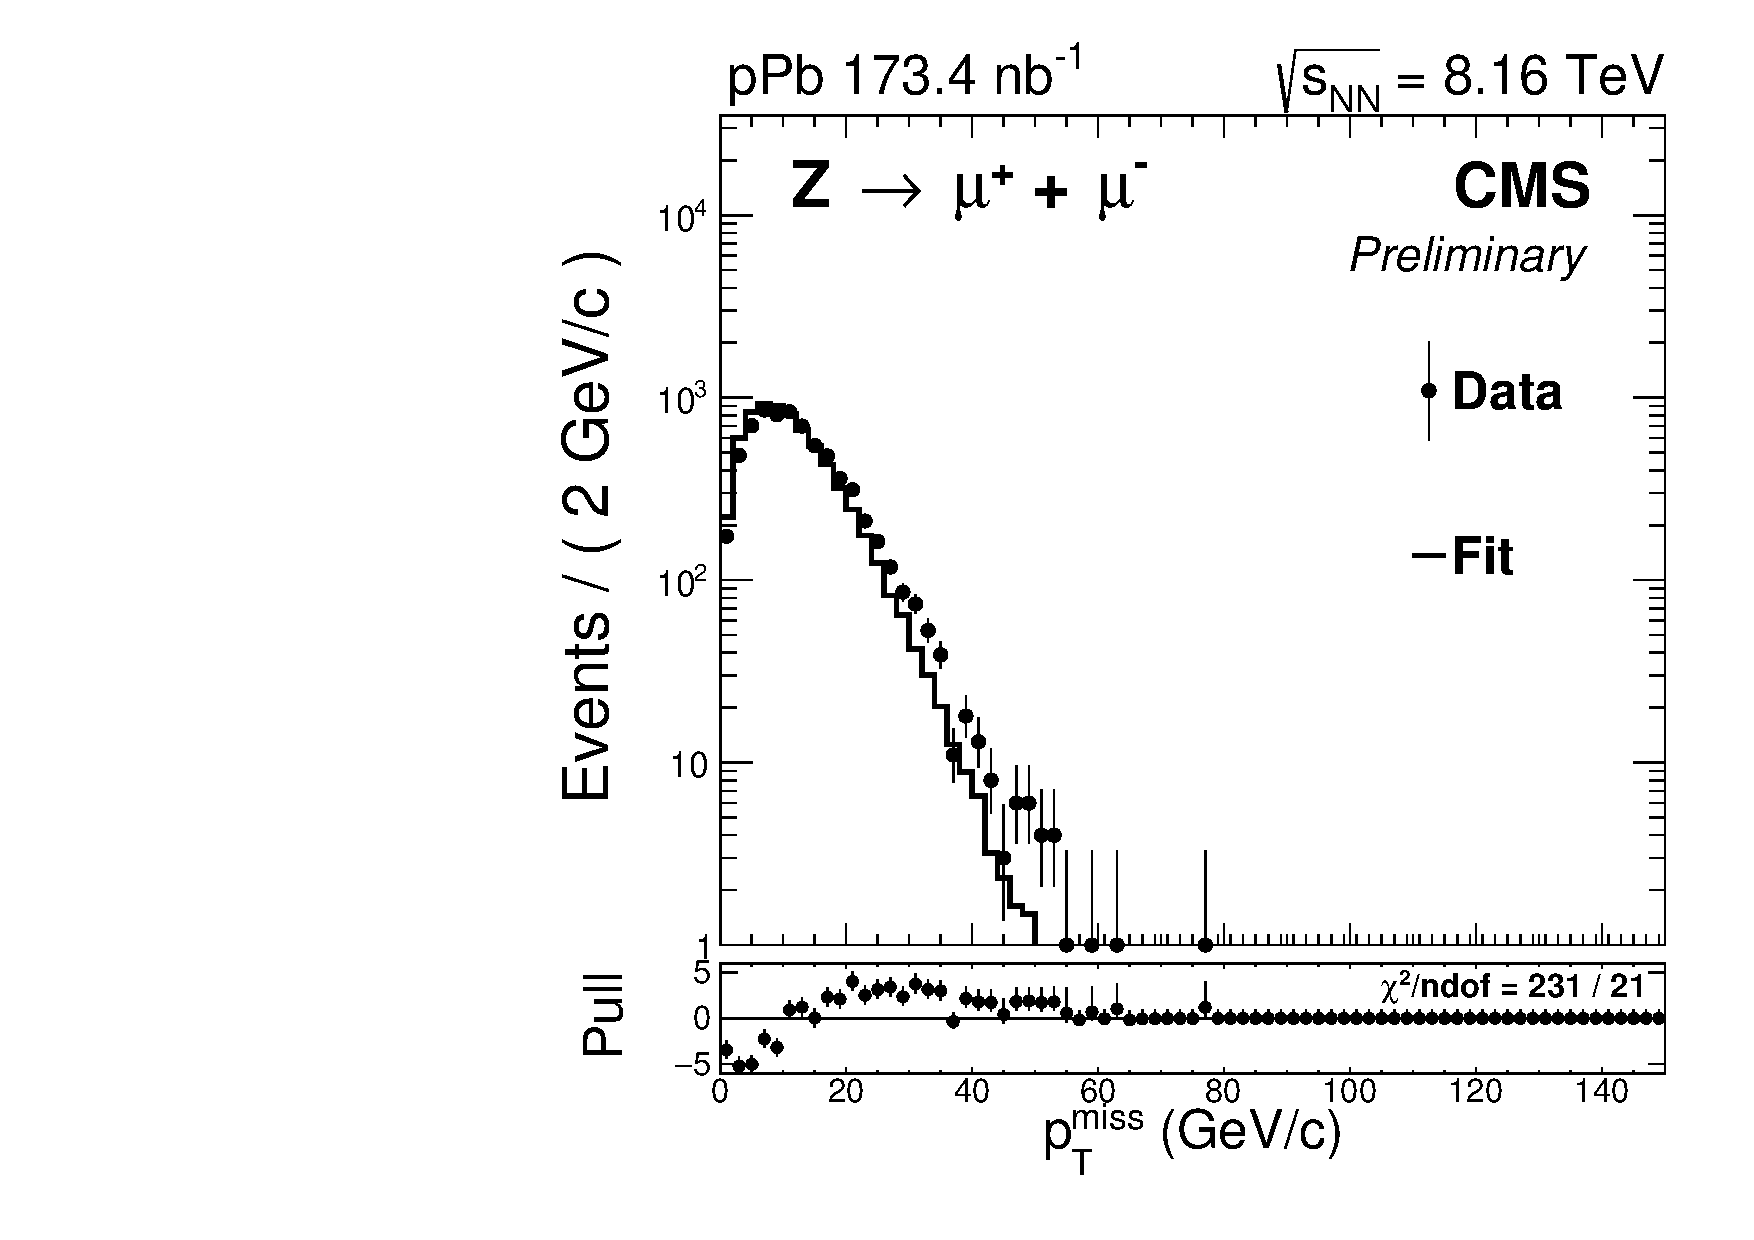
\includegraphics[width=0.45\textwidth]{Figures/WBoson/Analysis/Correction/Recoil/CheckFits/Z/METPF_RAW_HFBosonPTrew/PLOT_MET_DATA_ZToMuPl_PA_Model_TEMP_DY_MuEtaCM_-286_193_MuIso_0_15.pdf}
 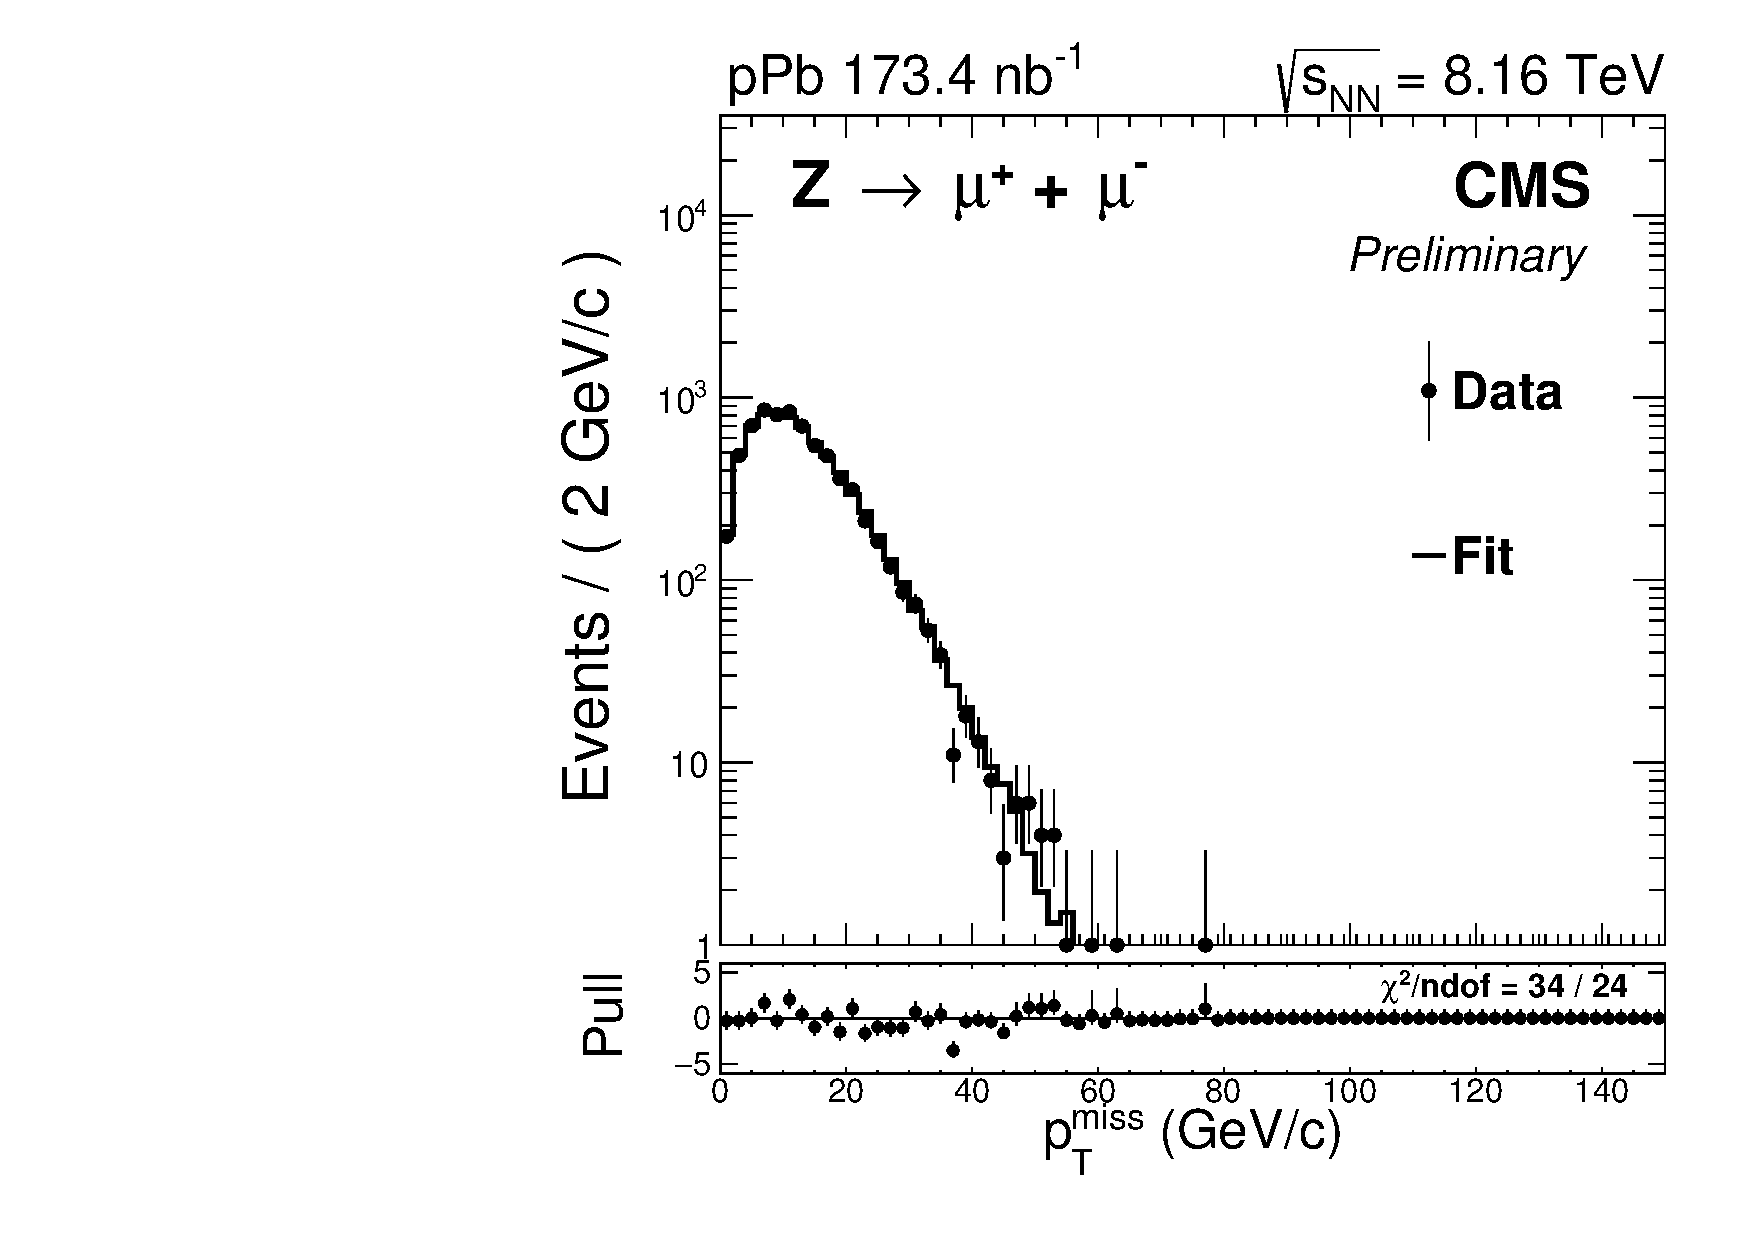
\includegraphics[width=0.45\textwidth]{Figures/WBoson/Analysis/Correction/Recoil/CheckFits/Z/Recoil_ScalingGauss/PLOT_MET_DATA_ZToMuPl_PA_Model_TEMP_DY_MuEtaCM_-286_193_MuIso_0_15.pdf}
 \caption{A comparison of the \ptmiss distribution from \ZToMuMu events between data and simulation, before (left) and after (right) calibrating the simulated recoil. The distributions of the simulated HF energy and generated \Z-boson \pt have been weighed.}
 \label{fig:recoilClosure}
\end{figure}


\paragraph{Impact of the recoil calibration in the signal region.} The \ptmiss distribution in the signal region is compared between data and the simulations. The fit to the data is performed following the signal extraction procedure described in \sect{sec:WBoson_Analysis_SignalExtraction}. The recoil corrections are applied to the electroweak simulations using both the nominal scaling method and the alternative smearing method, and the results are shown in \fig{fig:recoilCorrWreg}. Both the nominal and the alternative recoil calibrations improve significantly the agreement between the \ptmiss distribution extracted from data and simulations.

\begin{figure}[htb!]
 \centering
 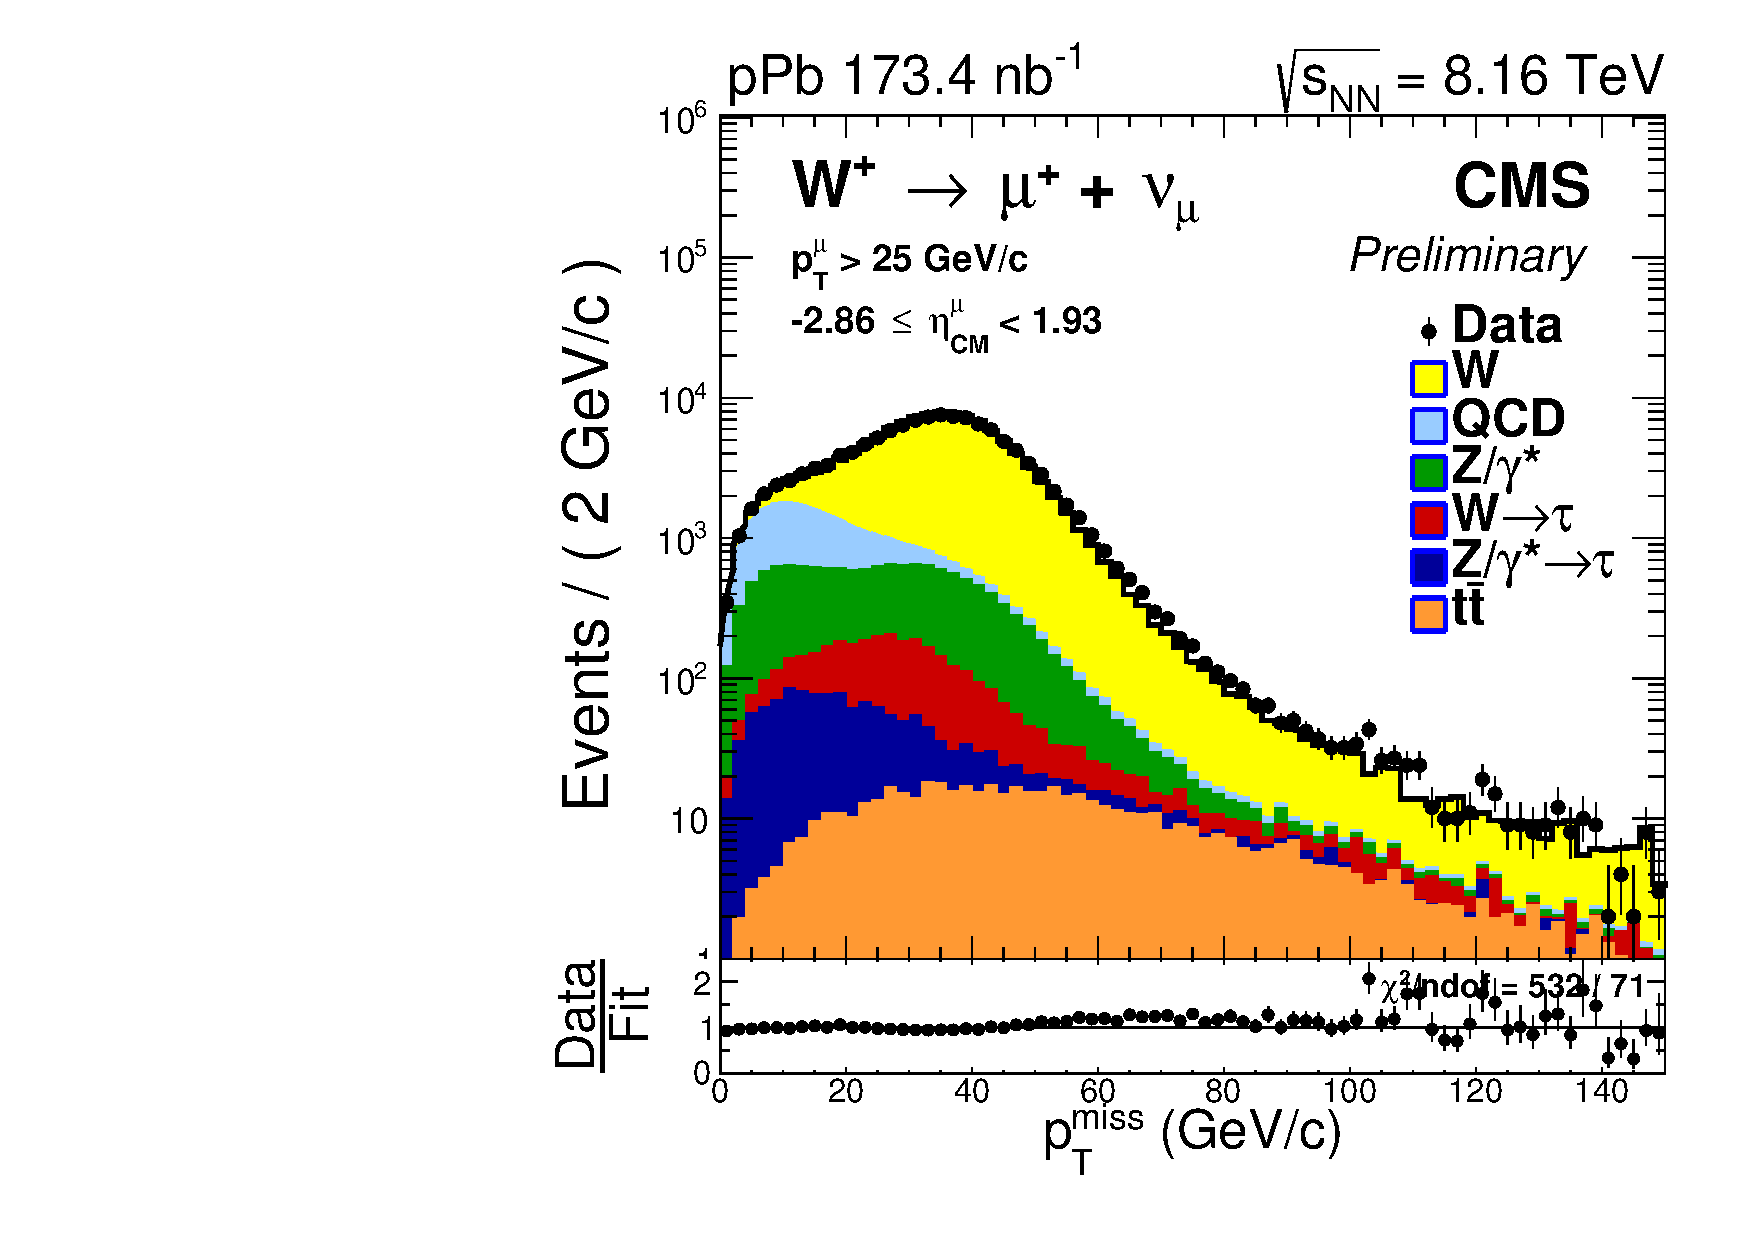
\includegraphics[width=0.45\textwidth]{Figures/WBoson/Analysis/Correction/Recoil/CheckFits/W/METPF_RAW_HFBosonPTrew/PLOT_MET_DATA_WToMuPl_PA_Model_TEMP_WDYDYToTauWToTauTTbar_ModifiedRayleigh_QCD_MuEtaCM_-286_193_MuIso_0_15.pdf}
 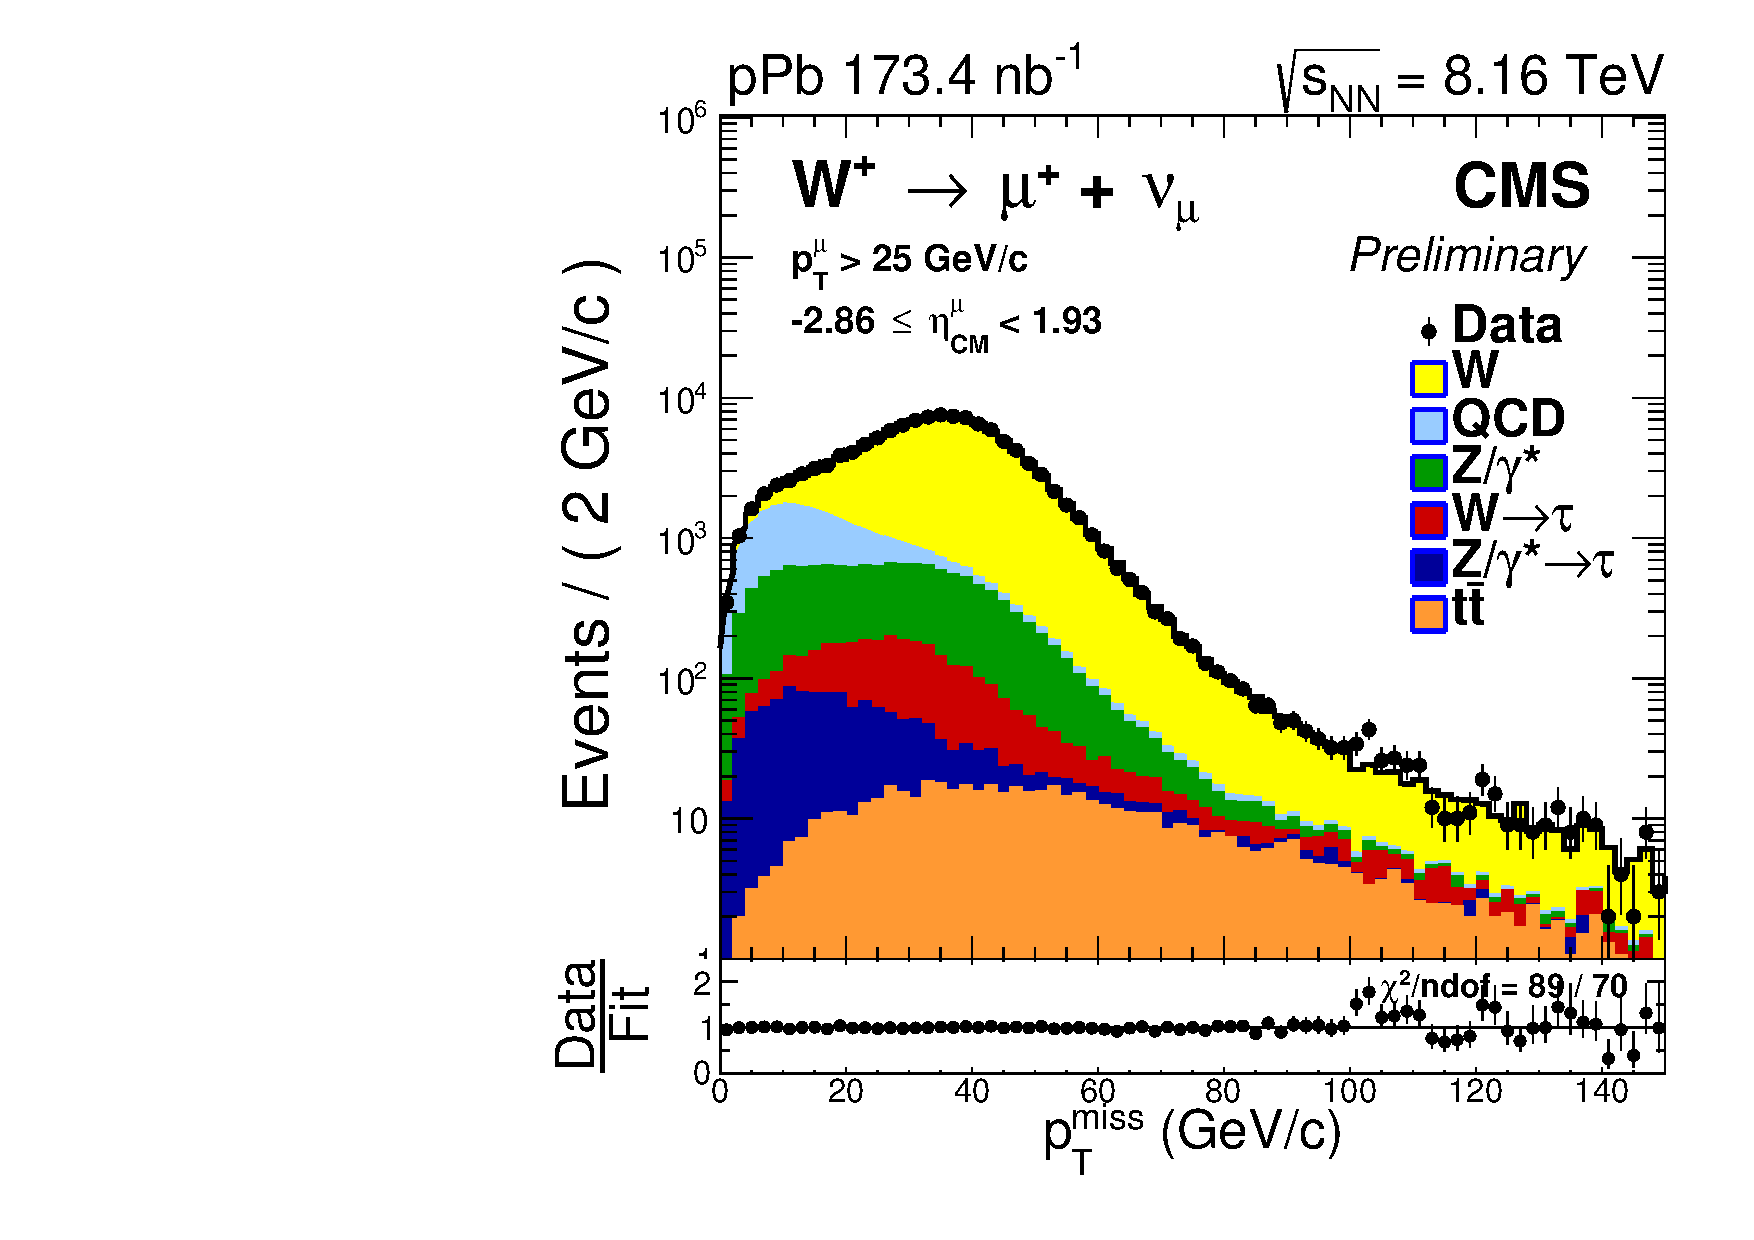
\includegraphics[width=0.45\textwidth]{Figures/WBoson/Analysis/Correction/Recoil/CheckFits/W/Recoil_ScalingGauss/PLOT_MET_DATA_WToMuPl_PA_Model_TEMP_WDYDYToTauWToTauTTbar_ModifiedRayleigh_QCD_MuEtaCM_-286_193_MuIso_0_15.pdf}
 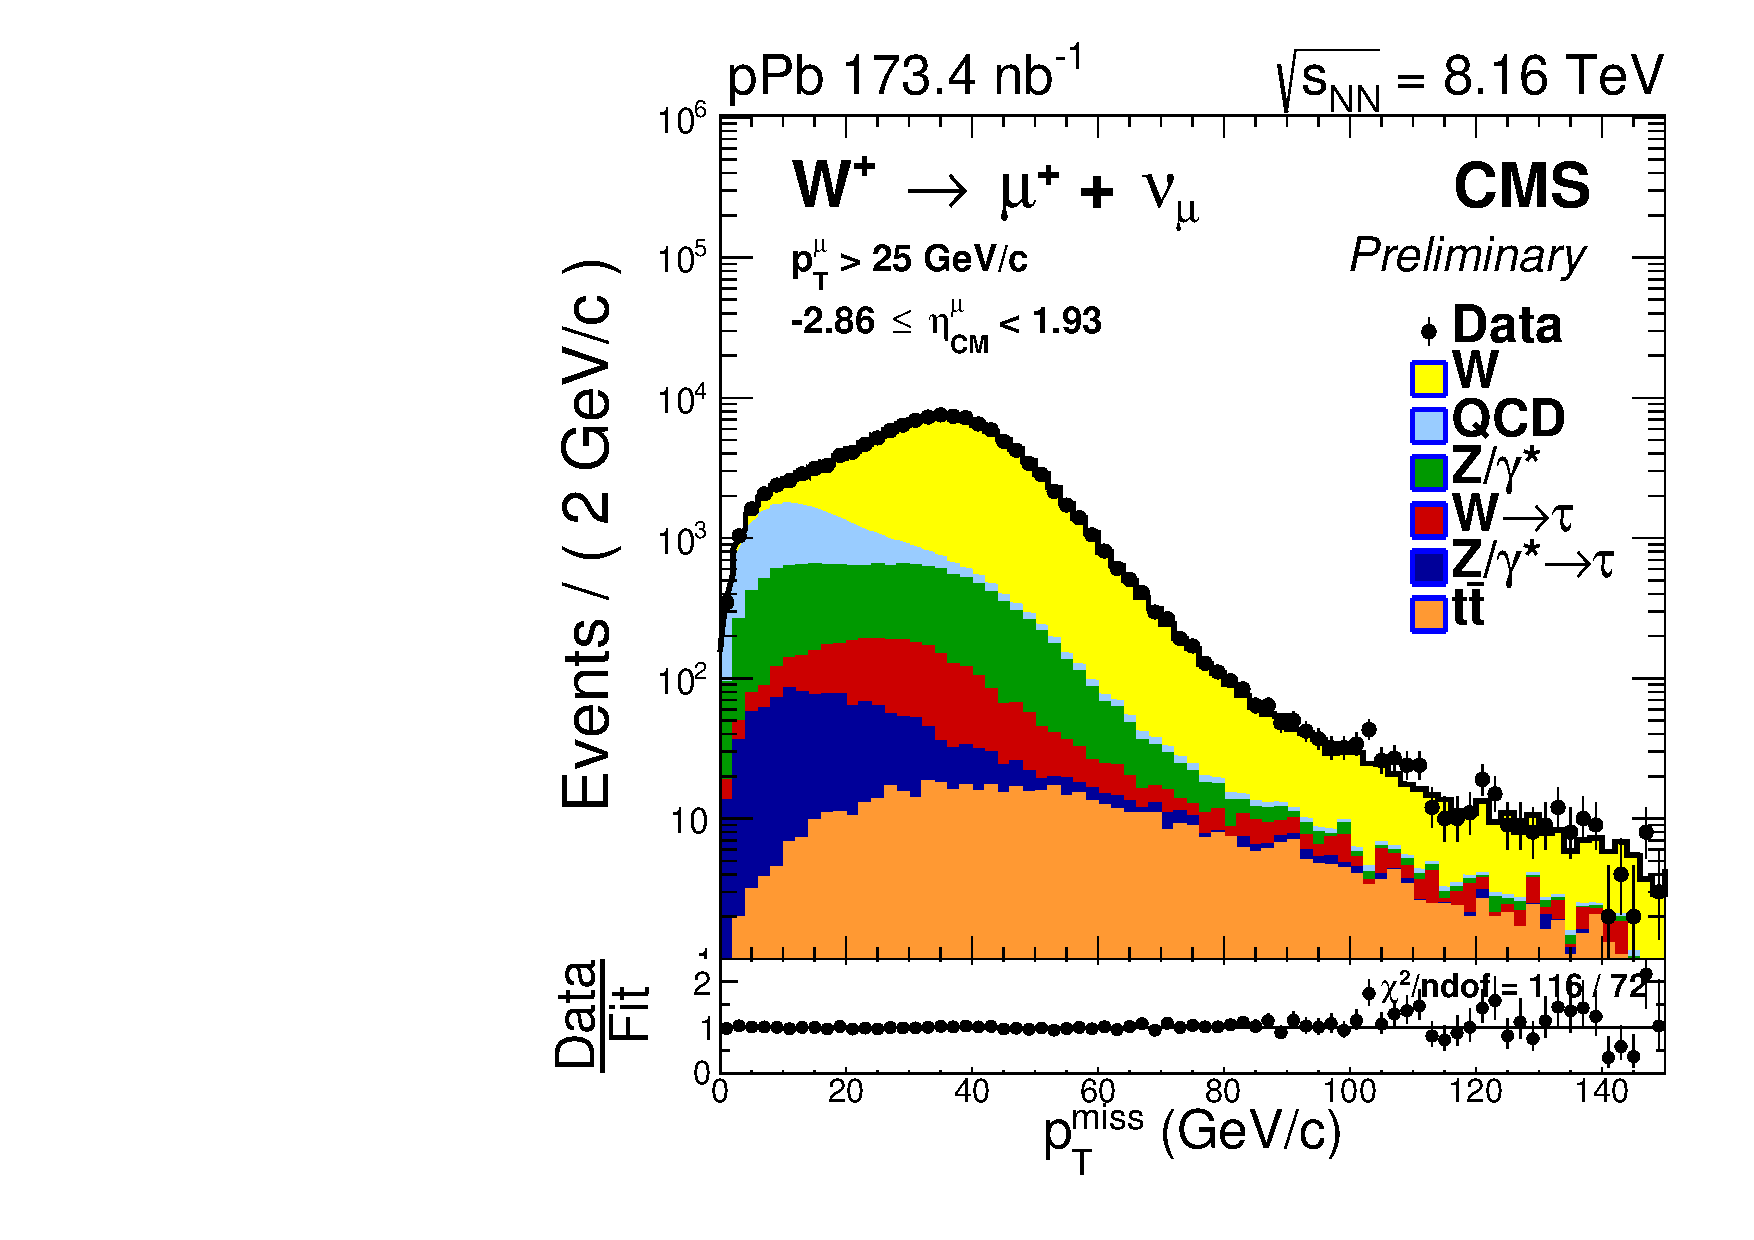
\includegraphics[width=0.45\textwidth]{Figures/WBoson/Analysis/Correction/Recoil/CheckFits/W/Recoil_Smearing/PLOT_MET_DATA_WToMuPl_PA_Model_TEMP_WDYDYToTauWToTauTTbar_ModifiedRayleigh_QCD_MuEtaCM_-286_193_MuIso_0_15.pdf}
 \caption{Comparison of the \ptmiss distribution in data and simulation for positive-charged muons in the  \etaMuCM-inclusive signal region. The results are shown before (top-left) and after (top-right) applying the recoil calibrations using the nominal scaling method. The result using the alternative smearing method (bottom) is also presented. The distributions of the simulated HF energy and generated \Z-boson \pt have been weighed.}
 \label{fig:recoilCorrWreg}
\end{figure}


% END OF SUBSECTION